\documentclass{article}
\usepackage{NotesTeX}

\renewcommand{\footnote}[1]{\sn{#1}}

\usepackage{amsmath,amssymb}
\usepackage{enumitem}
\usepackage{tcolorbox}
\usepackage{tikz-cd}
\usepackage{mathtools}
\usepackage{dsfont}
\usepackage{colortbl}
\usepackage{booktabs}
\usepackage{multirow}
\usepackage{longtable}
\usepackage{float}
\usepackage{comment}

\providecommand{\tightlist}{%
  \setlength{\itemsep}{0pt}\setlength{\parskip}{0pt}}

\renewcommand{\leq}{\leqslant}
\renewcommand{\geq}{\geqslant}

\usepackage{pgfplots}
\pgfplotsset{compat=1.17}
\usepackage{tikz-3dplot-circleofsphere}

\definecolor{primary}{RGB}{255,153,0}
\definecolor{secondary}{RGB}{51,102,136}

\usepackage{hyperref}
\hypersetup{linkcolor={secondary},urlcolor={primary}}
\usepackage[noabbrev,capitalise,nameinlink]{cleveref}
\crefformat{equation}{(#2#1#3)}


\newenvironment{idea}%
{\bigskip\noindent\begin{minipage}{\textwidth}\smallskip\begin{tcolorbox}[colback=gray!10,boxrule=0.01mm]}%
{\end{tcolorbox}\end{minipage}\bigskip}

\newtheorem*{scenario}{Scenario}

\tcolorboxenvironment{scenario}{
  boxrule=0pt,
  boxsep=0pt,
  colback={secondary!20},
  enhanced jigsaw,
  borderline west={2pt}{0pt}{secondary},
  sharp corners,
  before skip=10pt,
  after skip=10pt,
  breakable,
}

\newtheorem*{circuit}{Circuit}

\tcolorboxenvironment{circuit}{
  boxrule=0pt,
  boxsep=0pt,
  colback={primary!20},
  enhanced jigsaw,
  borderline west={2pt}{0pt}{primary},
  sharp corners,
  before skip=10pt,
  after skip=10pt,
  breakable,
}



\title{Lectures on Quantum Information Science}
\author{Artur Ekert and Tim Hosgood}
\date{Last updated: December 30, 2020}


\begin{document}

\setcounter{tocdepth}{2}
\tableofcontents

\providecommand{\xmapsto}[1]{\overset{#1}{\longmapsto}}
\providecommand{\bra}[1]{\langle#1|}
\providecommand{\ket}[1]{|#1\rangle}
\providecommand{\braket}[1]{\langle#1\rangle}
\providecommand{\proj}[1]{|#1\rangle\langle#1|}
\providecommand{\av}[1]{\braket{#1}}
\providecommand{\tr}{\operatorname{tr}}
\providecommand{\id}{\operatorname{id}}
\providecommand{\diag}[2]{\begin{bmatrix}#1&0\\0&#2\end{bmatrix}}
\renewcommand{\leq}{\leqslant}
\renewcommand{\geq}{\geqslant}

\hypertarget{introduction}{%
\section*{Introduction}\label{introduction}}
\addcontentsline{toc}{section}{Introduction}

In this series of lectures you will learn how inherently quantum phenomena, such as quantum interference and quantum entanglement, can make information processing more efficient and more secure, even in the presence of noise.

The interdisciplinary nature of this topic, combined with the diverse backgrounds that different readers have, means that some may find some particular chapters easy, while others find them difficult.
The following will be assumed as prerequisites: elementary probability theory, complex numbers, vectors and matrices, tensor products, and Dirac bra-ket notation.
A basic knowledge of quantum mechanics (especially in the simple context of finite dimensional state spaces, e.g.~state vectors, composite systems, unitary matrices, Born rule for quantum measurements) and some ideas from classical theoretical computer science (complexity theory) would be helpful, but is not at all essential.

\hypertarget{topics}{%
\subsection*{Topics}\label{topics}}
\addcontentsline{toc}{subsection}{Topics}

\begin{itemize}
\tightlist
\item
  Fundamentals of quantum theory

  \begin{itemize}
  \tightlist
  \item
    addition of probability amplitudes
  \item
    quantum interference
  \item
    mathematical description of states and evolution of closed quantum systems (Hilbert space, unitary evolution)
  \item
    measurements (projectors, Born rule)
  \item
    Pauli matrices
  \end{itemize}
\item
  Distinguishability of quantum states
\item
  The Bloch sphere

  \begin{itemize}
  \tightlist
  \item
    parametrisation
  \item
    action of quantum gates on the Bloch vector
  \end{itemize}
\item
  The definition of quantum entanglement (tensor product structure)
\item
  The no-cloning theorem and quantum teleportation
\item
  Quantum gates

  \begin{itemize}
  \tightlist
  \item
    phase gate
  \item
    Hadamard
  \item
    controlled-not
  \item
    SWAP
  \item
    the Hadamard-phase-Hadamard network
  \item
    phase ``kick-back'' induced by controlled-U
  \item
    phase ``kick-back'' induced by quantum Boolean function evaluation
  \end{itemize}
\item
  Quantum algorithms

  \begin{itemize}
  \tightlist
  \item
    Deutsch
  \item
    Bernstein-Vazirani
  \item
    Simon
  \end{itemize}
\item
  Bell's theorem

  \begin{itemize}
  \tightlist
  \item
    Quantum correlations
  \item
    CHSH inequality
  \item
    density matrices
  \item
    partial trace
  \item
    statistical mixture of pure states,
  \end{itemize}
\item
  Born rule for density matrices
\item
  Quantum entanglement in terms of density matrices
\item
  Completely positive maps

  \begin{itemize}
  \tightlist
  \item
    Kraus operators
  \item
    the Choi matrix
  \item
    positive versus completely positive maps
  \item
    partial-transpose
  \end{itemize}
\item
  The simple model of decoherence
\item
  Quantum error correction of bit-flip and phase-flip errors
\end{itemize}

\hypertarget{part-budding}{%
\part{Budding}\label{part-budding}}

\hypertarget{chapter1}{%
\section{Quantum interference: an overview}\label{chapter1}}

\begin{quote}
About complex numbers, called probability amplitudes, that, unlike probabilities, can cancel each other out, leading to quantum interference and qualitatively new ways of processing information.
\end{quote}

The classical theory of computation does not usually refer to physics.
Pioneers such as Alan Turing, Alonzo Church, Emil Post, and Kurt Gödel managed to capture the correct classical theory by intuition alone and, as a result, it is often falsely assumed that its foundations are self-evident and purely abstract.
They are not!\footnote{Computation is a physical process. Computation is a physical process. Computation is \ldots{}}

The concepts of information and computation can be properly formulated only in the context of a physical theory --- information is stored, transmitted and processed always by \emph{physical} means.
Computers are physical objects and computation is a physical process.
Indeed, any computation, classical or quantum, can be viewed in terms of physical experiments, which produce \textbf{outputs} that depend on initial preparations called \textbf{inputs}.
Once we abandon the classical view of computation as a purely logical notion independent of the laws of physics it becomes clear that whenever we improve our knowledge about physical reality, we may also gain new means of computation.
Thus, from this perspective, it is not very surprising that the discovery of quantum mechanics in particular has changed our understanding of the nature of computation.
In order to explain what makes quantum computers so different from their classical counterparts, we begin with the rudiments of quantum theory.

Some of what we say in this chapter will be repeated in later chapters, but usually in much more detail.
Feel free to think of this chapter as a sort of ``aeroplane tour'' of the rudiments, knowing that we will soon land on the ground to go out exploring by foot.

\hypertarget{two-basic-rules}{%
\subsection{Two basic rules}\label{two-basic-rules}}

Quantum theory, at least at some instrumental level, can be viewed as a modification of probability theory.
We replace positive numbers (probabilities) with complex numbers \(z\) (called \textbf{probability amplitudes}) such that the squares of their absolute values, \(|z|^2\), are interpreted as probabilities.

\begin{idea}

The correspondence between probability amplitude \(z\) and probability \(p=|z|^2\) is known as \textbf{Born's Rule}.

\end{idea}

The rules for combining amplitudes are very reminiscent of the rules for combining probabilities:

\begin{enumerate}
\def\labelenumi{\arabic{enumi}.}
\tightlist
\item
  Whenever something can happen in a sequence of independent steps, we multiply the amplitudes of each step.
\end{enumerate}

\begin{center}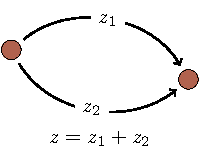
\includegraphics{quantum-info_files/figure-latex/unnamed-chunk-2-1} \end{center}

\begin{enumerate}
\def\labelenumi{\arabic{enumi}.}
\setcounter{enumi}{1}
\tightlist
\item
  Whenever something can happen in several alternative ways, we add the amplitudes for each separate way.
\end{enumerate}

\begin{center}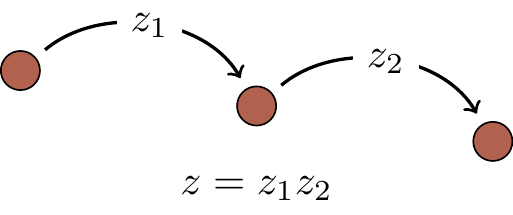
\includegraphics{quantum-info_files/figure-latex/unnamed-chunk-3-1} \end{center}

That's it!
These two rules are basically all you need to manipulate amplitudes in any physical process, no matter how complicated.\footnote{We will, however, amend the two rules later on when we touch upon particle statistics.}
They are universal and apply to any physical system, from elementary particles through atoms and molecules to white dwarfs stars.
They also apply to information, since, as we have already emphasised, information is physical.
The two rules look deceptively simple but, as you will see in a moment, their consequences are anything but trivial.

\hypertarget{quantum-interference-the-failure-of-probability-theory}{%
\subsection{Quantum interference: the failure of probability theory}\label{quantum-interference-the-failure-of-probability-theory}}

Modern mathematical probability theory is based on three axioms, proposed by Andrey Nikolaevich Kolmogorov (1903--1987) in his monograph with the impressive German title \emph{Grundbegriffe der Wahrscheinlichkeitsrechnung} (``Foundations of Probability Theory'').
The \textbf{Kolmogorov axioms} are simple and intuitive:\footnote{I always found it an interesting coincidence that the two basic ingredients of modern quantum theory, namely probability and complex numbers, were discovered by the same person, an extraordinary man of many talents: a gambling scholar by the name of Girolamo Cardano (1501--1576).}

\begin{enumerate}
\def\labelenumi{\arabic{enumi}.}
\tightlist
\item
  Once you identify all elementary outcomes, or events, you may then assign probabilities to them.
\item
  Probability is a number between \(0\) and \(1\), and an event which is certain has probability \(1\).
\item
  Last but not least, the probability of any event can be calculated using a deceptively simple rule --- the \textbf{additivity axiom}:
  \emph{Whenever an event can occur in several mutually exclusive ways, the probability for the event is the sum of the probabilities for each way considered separately.}
\end{enumerate}

Obvious, isn't it?
So obvious, in fact, that probability theory was accepted as a mathematical framework theory, a language that can be used to describe actual physical phenomena.
Physics should be able to identify elementary events and assign numerical probabilities to them.
Once this is done we may revert to mathematical formalism of probability theory.
The Kolmogorov axioms will take care of the mathematical consistency and will guide us whenever there is a need to calculate probabilities of more complex events.
This is a very sensible approach, apart from the fact that it does not always work!
Today, we know that probability theory, as ubiquitous as it is, fails to describe many common quantum phenomena.
In order to see the need for quantum theory let us consider a simple experiment in which probability theory fails to give the right predictions.

\hypertarget{the-double-slit-experiment}{%
\subsubsection{The double slit experiment}\label{the-double-slit-experiment}}

In a double slit experiment, a particle emitted from a source \(S\) can reach the detector \(D\) by taking two different paths, e.g.~through an upper or a lower slit in a barrier between the source and the detector.
After sufficiently many repetitions of this experiment we can evaluate the frequency of clicks in the detector \(D\) and show that it is inconsistent with the predictions based on probability theory.
Let us use the quantum approach to show how the discrepancy arises.

The particle emitted from a source \(S\) can reach detector \(D\) by taking two different paths, with amplitudes \(z_1\) and \(z_2\) respectively.
We may say that the upper slit is taken with probability \(p_1=|z_1|^2\) and the lower slit with probability \(p_2=|z_2|^2\).
These are two mutually exclusive events.
With the two slits open, probability theory declares (by the additivity axiom) that the particle should reach the detector with probability \(p_1+p_2= |z_1|^2+|z_2|^2\).
But this is not what happens experimentally!

Following the ``quantum rules'', first we add the amplitudes and then we square the absolute value of the sum to get the probability.
Thus, the particle will reach the detector with probability
\begin{equation}
\begin{aligned}
  p &= |z|^2
\\& = |z_1 + z_2|^2
\\& = |z_1|^2 + |z_2|^2
      + z_1^\star z_2 + z_1 z_2^\star
\\& = p_1 + p_2
      + |z_1||z_2|\left(
        e^{i(\varphi_2-\varphi_1)}
        + e^{-i(\varphi_2-\varphi_1)}
      \right)
\\& = p_1 + p_2
      + 2 \sqrt{p_1 p_2} \cos(\varphi_2-\varphi_1)
\\& = p_1 + p_2 + \mbox{interference terms}
\end{aligned}
\label{eq:interference}
\end{equation}
where we have expressed the amplitudes in their polar forms
\[
\begin{aligned}
  z_1 &= |z_1|e^{i\varphi_1}
\\z_2 &= |z_2|e^{i\varphi_2}.
\end{aligned}
\]
The appearance of the interference terms marks the departure from the classical theory of probability.
The probability of any two seemingly mutually exclusive events is the sum of the probabilities of the individual events, \(p_1 + p_2\), \emph{modified} by the \textbf{interference term} \(2 \sqrt{p_1p_2}\cos(\varphi_2-\varphi_1)\).
Depending on the \textbf{relative phase} \(\varphi_2-\varphi_1\), the interference term can be either negative (which we call \textbf{destructive} interference) or positive (\textbf{constructive} interference), leading to either suppression or enhancement of the total probability \(p\).

The algebra is simple; our focus is on the physical interpretation.
Firstly, note that the important quantity here is the \emph{relative} phase \(\varphi_2-\varphi_1\) rather than the individual values \(\varphi_1\) and \(\varphi_2\).
This observation is not trivial at all.
If a particle reacts only to the difference of the two phases, each pertaining to a separate path, then it must have, somehow, experienced the two paths, right?
Thus we cannot say that the particle has travelled either through the upper or the lower slit, because it has travelled through \emph{both}.
In the same way, quantum computers follow, in some tangible way, all computational paths simultaneously, producing answers that depend on all these alternative calculations.
Weird, but this is how it is!
Secondly, what has happened to the additivity axiom in probability theory --- what is wrong with it?
One thing that is wrong is the assumption that the processes of taking the upper or the lower slit are mutually exclusive.
In reality, as we have just mentioned, the two transitions \emph{both occur}, simultaneously.
However, we cannot learn this from probability theory, or any other a priori mathematical construct.
There is no fundamental reason why Nature should conform to the additivity axiom.
\footnote{According to the philosopher Karl Popper (1902--1994) a theory is genuinely scientific only if it is possible, in principle, to establish that it is false. Genuinely scientific theories are never finally confirmed because no matter how many confirming observations have been made observations that are inconsistent with the empirical predictions of the theory are always possible.}
We find out how nature works by making intelligent guesses, running experiments, checking what happens and formulating physical theories.
If our guess disagrees with experiments then it is wrong, so we try another intelligent guess, and another, etc.
Right now, quantum theory is the best guess we have: it offers good explanations and predictions that have not been falsified by any of the existing experiments.
This said, be assured that one day quantum theory will be falsified and we will have to start guessing again.

\hypertarget{superpositions}{%
\subsection{Superpositions}\label{superpositions}}

Amplitudes are more than just tools for calculating probabilities: they tell us something about physical reality.
When we deal with probabilities, we may think about them as numbers that quantify our lack of knowledge.
Indeed, when we say that a particle goes through the upper or the lower slit with some respective probabilities it does go through one of the two slits, we just do not know which one.
In contrast, according to quantum theory, a particle that goes through the upper and the lower slit with certain amplitudes does explore both of the two paths, not just one of them.
This is a statement about a real physical situation, about something that is out there and something we can experiment with.
The assumption that the particle goes through one of the two slits, but we do not know which one, is inconsistent with the experimental observations.
We have to accept that apart from some easy to visualise states, also known as the basis states, such as the particle at the upper slit or the particle at the lower slit, there are infinitely many other states, all of them equally real, in which the particle is in a \emph{superposition} of the two basis states.
This rather bizarre picture of reality is the best we have at the moment, and it works, at least for now. Physicists write such states as
\footnote{Dirac notation will likely be familiar to physicists, but may look odd to mathematicians or computer scientists. Love it or hate it (and I suggest the former), the notation is so common that you simply have no choice but to learn it, especially if you want to study anything related to quantum theory.}
\[
|\psi\rangle=\alpha |\text{at the upper slit}\rangle +\beta |\text{at the lower slit}\rangle,
\]
meaning the particle at the upper slit with amplitude \(\alpha\) and at the lower slit with amplitude \(\beta\). Mathematically, you can think about this expression as a vector \(|\psi\rangle\) in a two-dimensional complex vector space written in terms of the two basis vectors \(|\text{at the upper slit}\rangle\) and \(|\text{at the lower slit}\rangle\). You can also write this vector as a column vector with two complex entries \(\alpha\) and \(\beta\), but then you have to explain the physical meaning of the basis states. Here, we use the \(|\cdot\rangle\) notation, introduced by Paul Dirac in the early days of the quantum theory as a useful way to write and manipulate vectors. In Dirac notation you can put into the box \(|\phantom{0}\rangle\) anything that serves to specify what the vector is. It could be \(|\uparrow\rangle\) for spin up and \(|\downarrow\rangle\) for spin down, or \(|0\rangle\) for a quantum bit holding logical \(0\) and \(|1\rangle\) for a quantum bit holding logical \(1\), etc. As we shall see soon, there is much more to this notation.

\hypertarget{interferometers}{%
\subsection{Interferometers}\label{interferometers}}

Many modern interference experiments are performed using internal degrees of freedom of atoms and ions. For example, \textbf{Ramsey interferometry}, named after American physicist Norman Ramsey, is a generic name for an interference experiment in which atoms are sent through two separate resonant interaction zones, known as \textbf{Ramsey zones}, separated by an intermediate dispersive interaction zone.

Many beautiful experiments of this type were carried out in the 1990s in Serge Haroche's lab at the Ecole Normale Supérieure in Paris. Rubidium atoms were sent through two separate interaction zones (resonant interaction in the first and the third cavity) separated by a phase inducing dispersive interaction zone (the central cavity). The atoms were subsequently measured, via a selective ionisation, and found to be in one of the two preselected energy states, here labeled as \(|0\rangle\) and \(|1\rangle\). The fraction of atoms found in states \(|0\rangle\) or \(|1\rangle\) showed a clear dependence on the phase shifts induced by the dispersive interaction in the central cavity. In 2012 Serge Haroche and Dave Wineland shared the Nobel Prize in physics for ``ground-breaking experimental methods that enable measuring and manipulation of individual quantum systems.''



\begin{figure}[H]

{\centering 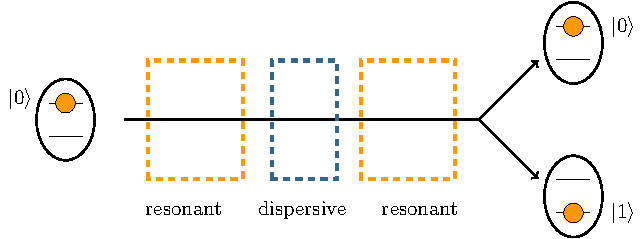
\includegraphics{quantum-info_files/figure-latex/ramsey-figure-1} 

}

\caption{A schematic diagram of a Ramsey interference experiment.}\label{fig:ramsey-figure}
\end{figure}

The three rectangular boxes in Figure \ref{fig:ramsey-figure} represent three cavities, each cavity being an arrangement of mirrors which traps electromagnetic field (think about standing waves in between two mirrors).
The oval shapes represent rubidium atoms with two preselected energy states labelled as \(|0\rangle\) and \(|1\rangle\).
Each atom is initially prepared in a highly excited internal energy state \(|0\rangle\) and zips through the three cavities, from the left to the right.
In each cavity the atom interacts with the cavity field.
The first and the third cavities are, for all theoretical purposes, identical.
Their frequencies are tuned to the resonant frequency of the atom, and the atom exchanges energy with the cavity, going back and forth between its energy states \(|0\rangle\) and \(|1\rangle\).
In contrast, in the second (central) cavity, the atom undergoes the so-called dispersive interaction: it is too off resonance to exchange energy with the field but its energy states ``feel'' the field and acquire phase shifts.
After experiencing this well timed sequence of resonant--dispersive--resonant interactions, the energy of the atom is measured and the atom is found to be either in state \(|0\rangle\) or state \(|1\rangle\).
The fraction of atoms that is found in state \(|0\rangle\) or \(|1\rangle\) shows a clear dependence on the phase shifts induced by the dispersive interaction in the central cavity.

We can understand this interference better if we follow the two internal states of the atom as it moves through the three cavities.



\begin{figure}[H]

{\centering 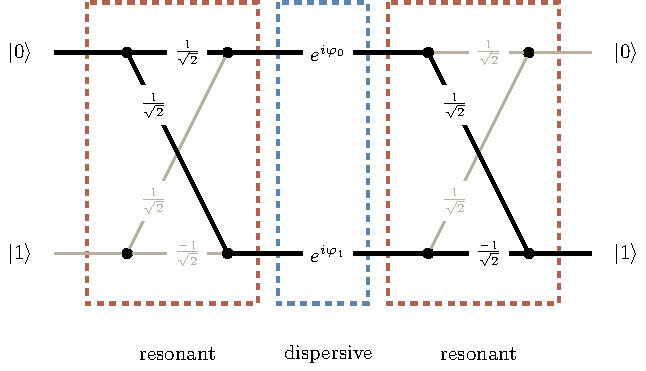
\includegraphics{quantum-info_files/figure-latex/ramsey-figure-2-1} 

}

\caption{The Ramsey interferometer represented as an abstract diagram. It should be read from left to right. The line segments represent transitions between the two states, \(|0\rangle\) and \(|1\rangle\), and the numbers are the corresponding probability amplitudes.}\label{fig:ramsey-figure-2}
\end{figure}

Suppose we are interested in the probability that the atom, initially in state \(|0\rangle\), will be found, after completing its journey through the three cavities, in state \(|1\rangle\).
As you can see in Figure \ref{fig:ramsey-figure-2}, this can happen in two ways, as indicated by the two red paths connecting the input state \(|0\rangle\) on the left with the output state \(|1\rangle\) on the right.
Again, let \(U_{ij}\) denote the probability amplitude that input \(|j\rangle\) generates output \(|i\rangle\) (for \(i,j=0,1\)).
We can see from the diagram that
\[
  \begin{aligned}
    U_{10}
    &= \frac{1}{\sqrt2} e^{i\varphi_0}\frac{1}{\sqrt2} + \frac{1}{\sqrt2} e^{i\varphi_1}\frac{-1}{\sqrt2}
  \\&= \frac12 e^{i\varphi_0} - \frac12 e^{i\varphi_1}
  \\&= -ie^{i\varphi/2}\sin\frac{\varphi}{2},
  \end{aligned}
\]
where \(\varphi = \varphi_0-\varphi_1\) is the relative phase.
The corresponding probability reads\footnote{From the classical probability theory perspective the resonant interaction induces a random switch between \(|0\rangle\) and \(|1\rangle\) (why ?) and the dispersive interaction has no effect on these two states (why ?). Hence, one random switch followed by another random switch gives a random switch, right, which gives \(\frac12\) for the probability that input \(|0\rangle\) becomes output \(|1\rangle\).}
\[
  \begin{aligned}
    P_{10}
    &= \vert U_{10}\vert^2
  \\&= \left\vert \frac12 e^{i\varphi_0} - \frac12 e^{i\varphi_1}\right\vert^2
  \\&= \frac12 - \frac12\cos\varphi.
  \end{aligned}
\]
You should recognise the first term, \(\frac12\), as the ``classical'' probability and the second one, \(-\frac12\cos\varphi\), as the interference term.
We can repeat such calculations for any other pair of input--output states.
This approach works fine here but, in general, tracking all possible paths in evolving quantum systems can become messy when the number of input and output states increases.
There is, however, a neat way of doing it via matrix multiplication.

The effect of each interaction on atomic states can be described by a matrix of transition amplitudes, as illustrated in Figure \ref{fig:interference-matrix}.
Then a sequence of independent interactions is described by the product of these matrices.
\[
  \begin{aligned}
    U &=
    \begin{bmatrix}
      \frac{1}{\sqrt2} & \frac{1}{\sqrt2}
    \\\frac{1}{\sqrt2} & \frac{-1}{\sqrt2}
    \end{bmatrix}
    \begin{bmatrix}
      e^{i\varphi_0} & 0
    \\0 & e^{i\varphi_1}
    \end{bmatrix}
    \begin{bmatrix}
      \frac{1}{\sqrt2} & \frac{1}{\sqrt2}
    \\\frac{1}{\sqrt2} & \frac{-1}{\sqrt2}
    \end{bmatrix}
  \\&= e^{i\frac{\varphi_0+\varphi_1}{2}}
    \begin{bmatrix}
      \cos\frac{\varphi}{2} & -i\sin\frac{\varphi}{2}
    \\\ -i\sin\frac{\varphi}{2}& \cos\frac{\varphi}{2}
    \end{bmatrix},
  \end{aligned}
\]
where \(\varphi = \varphi_0-\varphi_1\).



\begin{figure}[H]

{\centering 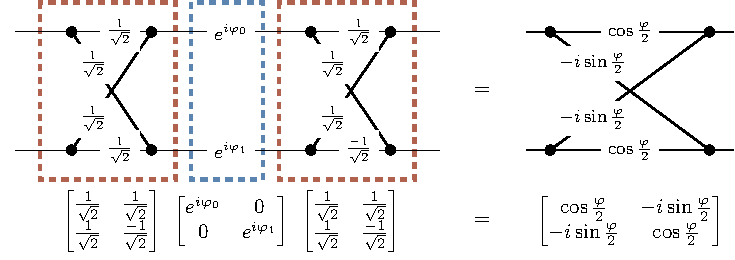
\includegraphics{quantum-info_files/figure-latex/interference-matrix-1} 

}

\caption{The Ramsey interferometer represented as an abstract diagram (matrix approach). Here we have omitted the \(|0\rangle\) and \(|1\rangle\) labels, just to simply the diagram. We also ignore the global phase factor of \(e^{i\frac{\varphi_0+\varphi_1}{2}}\).}\label{fig:interference-matrix}
\end{figure}

In general, quantum operation \(A\) followed by another quantum operation \(B\) is a quantum operation described by the matrix product \(BA\) (watch the order of matrices).
Indeed, the expression \((BA)_{ij}=\sum_k B_{ik}A_{kj}\) is the sum over amplitudes that input \(|j\rangle\) generates output \(|i\rangle\) via a specific intermediate state \(|k\rangle\).
As you can see, the matrix approach is a wonderful bookkeeping tool for in one swap it takes care of both multiplying and adding probability amplitudes corresponding to all the contributing paths.

\hypertarget{qubits-gates-and-circuits}{%
\subsection{Qubits, gates, and circuits}\label{qubits-gates-and-circuits}}

Atoms, trapped ions, molecules, nuclear spins and many other quantum objects with two pre-selected basis states labeled as \(|0\rangle\) and \(|1\rangle\) (from now on we will call such objects quantum bits or \textbf{qubits}) can be used to implement simple quantum interference.
There is no need to learn about physics behind these diverse technologies if all you want is to understand the basics of quantum theory.
We may now conveniently forget about any specific experimental realisation of a qubit and represent a generic \textbf{single qubit interference} graphically as a \textbf{circuit diagram}:\footnote{Do not confuse the interference diagrams of Figure \ref{fig:ramsey-figure} and Figure \ref{fig:interference-matrix} with the circuit diagram. In the circuit diagrams, which we will use a lot from now on, a single qubit is represented by a single line.}

\begin{center}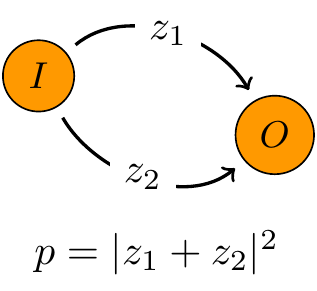
\includegraphics{quantum-info_files/figure-latex/unnamed-chunk-4-1} \end{center}

This diagram should be read from left to right.
The horizontal line represents a qubit that is inertly carried from one quantum operation to another. We often call this line a \textbf{quantum wire}.
The wire may describe translation in space (e.g.~atoms travelling through cavities) or translation in time (e.g.~a sequence of operations performed on a trapped ion).
The boxes or circles on the wire represent elementary quantum operations, called \textbf{quantum logic gates}.
Here we have two types of gates: two Hadamard gates \(H\) (think about resonant interactions) and one phase gate \(P_\varphi\) (think about dispersive interaction), where\footnote{Global phase factors are irrelevant, it is the relative phase \(\varphi =\varphi_1-\varphi_0\) that matters. In a single qubit phase gate we usually factor out \(e^{i\varphi_0}\), which leaves us with the two diagonal entries: \(1\) and \(e^{i\varphi}\).}
\[
H=\begin{bmatrix}
    \frac{1}{\sqrt2} & \frac{1}{\sqrt2}
  \\\frac{1}{\sqrt2} & \frac{-1}{\sqrt2}
  \end{bmatrix}
  \quad\text{and}\quad
P_\varphi  = \begin{bmatrix}
    1 & 0
  \\0 & e^{i\varphi}
  \end{bmatrix}.
\]

The input qubits appear as state vectors on the left side of circuit diagrams, and the output qubits as state vectors on the right.
The product of the three matrices \(HP_\varphi H\) (see Figure \ref{fig:interference-matrix}) describes the action of the whole circuit: it maps input state vectors to output state vectors\footnote{\(HP_\varphi H =\begin{bmatrix}\cos\frac{\varphi}{2} & -i\sin\frac{\varphi}{2}\\\ -i\sin\frac{\varphi}{2}& \cos\frac{\varphi}{2}\end{bmatrix}\).}:
\[
  \begin{array}{lcr}
    |0\rangle & \mapsto & \cos\frac{\varphi}{2}|0\rangle - i\sin\frac{\varphi}{2}|1\rangle,
  \\|1\rangle
    & \mapsto
    &- i\sin\frac{\varphi}{2}|0\rangle + \cos\frac{\varphi}{2}|1\rangle.
  \end{array}
\]

\hypertarget{quantum-decoherence}{%
\subsection{Quantum decoherence}\label{quantum-decoherence}}

We do need quantum theory to describe many physical phenomena, but, at the same time, there are many other phenomena where the classical theory of probability works pretty well.
We hardly see quantum interference on a daily basis.
Why?
The answer is \textbf{decoherence}.
The addition of probability amplitudes, rather than probabilities, applies to physical systems which are completely isolated.
However, it is almost impossible to isolate a complex quantum system, such as a quantum computer, from the rest of the world.
There will always be spurious interactions with the environment, and when we add amplitudes, we have to take into account not only different configurations of the physical system at hand, but also different configurations of the environment.

For example, consider an isolated system composed of a quantum computer and its environment.
The computer is prepared in some input state \(I\) and generates output \(O\).
Let us look at the following two scenarios:

\begin{enumerate}
\def\labelenumi{\arabic{enumi}.}
\tightlist
\item
  \emph{The computer is isolated and quantum computation does not affect the environment.}
  The computer and the environment evolve independently from each other and, as a result, the environment does not hold any physical record of how the computer reached output \(O\).
  In this case we add the amplitudes for each of the two alternative computational paths.
\end{enumerate}

\begin{center}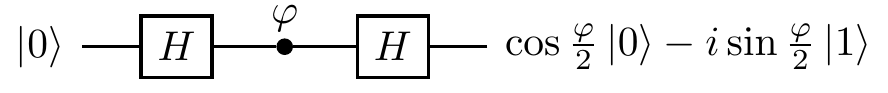
\includegraphics{quantum-info_files/figure-latex/unnamed-chunk-5-1} \end{center}

\begin{enumerate}
\def\labelenumi{\arabic{enumi}.}
\setcounter{enumi}{1}
\tightlist
\item
  \emph{Quantum computation affects the environment.}
  The environment now holds a physical record of how the computer reached output \(O\), which results in two final states of the composed system (computer + environment) which we denote \(O_1\) and \(O_2\).
  We add the probabilities for each of the two alternative computational paths.
\end{enumerate}

\begin{center}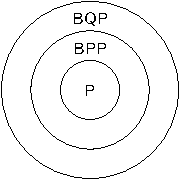
\includegraphics{quantum-info_files/figure-latex/unnamed-chunk-6-1} \end{center}

When quantum computation affects the environment, we have to include the environment in our analysis for it now takes part in the computation.
Depending on which computational path was taken, the environment may end up in two distinct states.
The computer itself may show output \(O\), but when we include the environment we have not one, but two outputs, \(O_1\) and \(O_2\), denoting, respectively, ``computer shows output \(O\) and the environment knows that path \(1\) was taken'' and ``computer shows output \(O\) and the environment knows that path \(2\) was taken''.
There are no alternative ways of reaching \(O_1\) or \(O_2\), hence there is no interference, and the corresponding probabilities read \(p_1=|z_1|^2\) for \(O_1\), and \(p_2=|z_2|^2\) for \(O_2\).
The probability that the computer shows output \(O\), regardless the state of the environment, is the sum of of the two probabilities: \(p=p_1+p_2\).
We have lost the interference term and any advantages of quantum computation along with it.
In the presence of decoherence the interference formula \eqref{eq:interference} is modified and reads
\[
p
= p_1 + p_2 + 2 v \sqrt{p_1 p_2}\cos (\varphi_2-\varphi_1),
\]
where the parameter \(v\), called the \textbf{visibility} of the interference pattern, ranges from \(0\) (the environment can perfectly distinguish between the two paths, total decoherence, no interference) to \(1\) (the environment cannot distinguish between the two paths, no decoherence, full interference), with the values in between corresponding to partial decoherence.

\begin{center}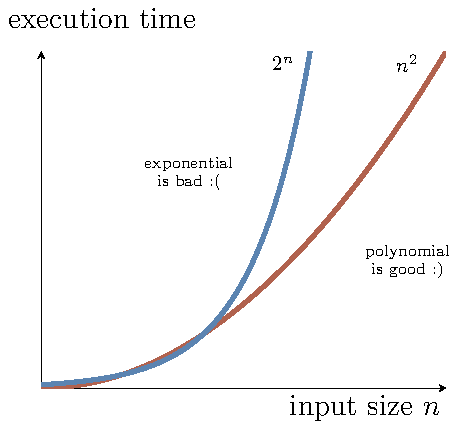
\includegraphics{quantum-info_files/figure-latex/unnamed-chunk-7-1} \end{center}

We shall derive this formula later on, and you will see that \(v\) quantifies the degree of distinguishability between \(O_1\) and \(O_2\).
The more the environment knows about which path was taken the less interference we see.

\begin{idea}

Decoherence suppresses quantum interference.

\end{idea}

Decoherence is chiefly responsible for our classical description of the world --- without interference terms we may as well add probabilities instead of amplitudes.
While decoherence is a serious impediment to building quantum computers, depriving us of the power of quantum interference, it is not all doom and gloom: there are clever ways around decoherence, such as quantum error correction and fault-tolerant methods we will meet later.

\hypertarget{computation-deterministic-probabilistic-and-quantum}{%
\subsection{Computation: deterministic, probabilistic, and quantum}\label{computation-deterministic-probabilistic-and-quantum}}

Take one physical bit or a qubit.
It has two logical states: \(|0\rangle\) and \(|1\rangle\).
Bring another qubit and the combined systems has four logical states \(|00\rangle, |01\rangle,|10\rangle\) and \(|11\rangle\).
In general \(n\) qubits will give us \(2^n\) states representing all possible binary strings of length \(n\).
It is important to use subsystems --- here qubits --- rather than one chunk of matter, for operating on at most \(n\) qubits we can reach any of the \(2^n\) states of the composed system.
Now, let the qubits interact in a controllable fashion.
We are computing.
Think about computation as a physical process that evolves a prescribed initial configuration of a computing machine, called \textbf{\(\texttt{INPUT}\)}, into some final configuration, called \textbf{\(\texttt{OUTPUT}\)}.
We shall refer to the configurations as \textbf{states}.
Figure \ref{fig:deterministic-computation} shows five consecutive computational steps performed on four distinct states.

\begin{figure}[H]

{\centering 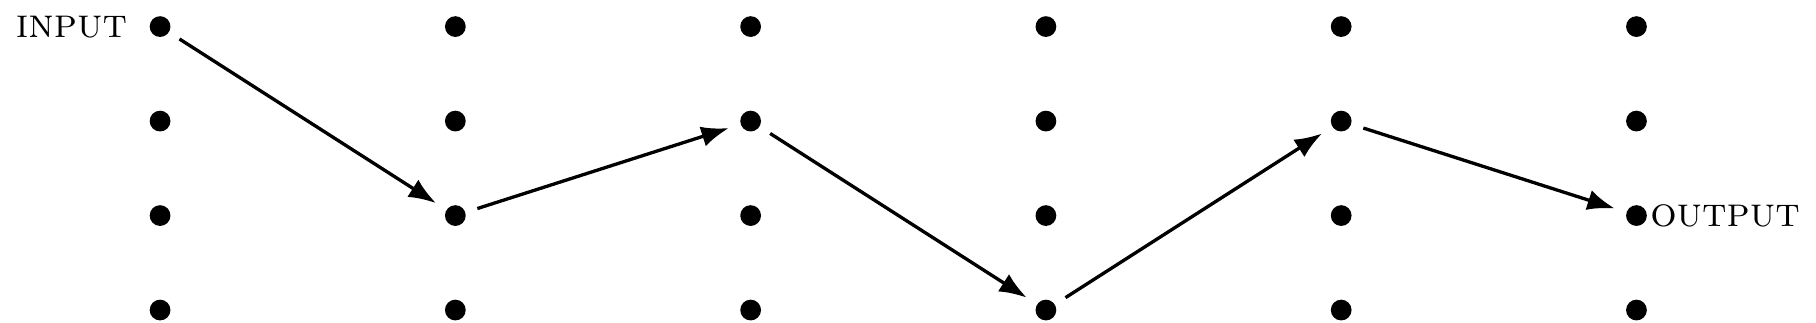
\includegraphics{quantum-info_files/figure-latex/deterministic-computation-1} 

}

\caption{Deterministic computation.}\label{fig:deterministic-computation}
\end{figure}

That computation was \textbf{deterministic}: every time you run it with the same input, you get the same output.
But a computation does not have to be deterministic --- we can augment a computing machine by allowing it to ``toss an unbiased coin'' and to choose its steps randomly.
It can then be viewed as a directed\footnote{So we read left to right, and omit the arrowheads.} tree-like graph where each node corresponds to a state of the machine, and each edge represents one step of the computation, as shown in Figure \ref{fig:probabilistic-computation}

\begin{figure}[H]

{\centering 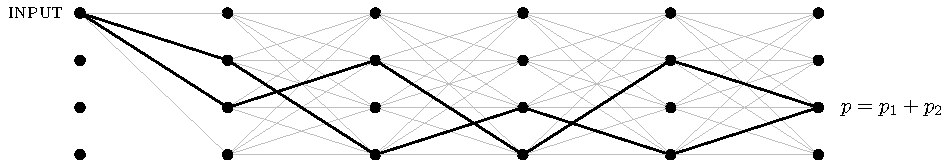
\includegraphics{quantum-info_files/figure-latex/probabilistic-computation-1} 

}

\caption{Probabilistic computation.}\label{fig:probabilistic-computation}
\end{figure}

The computation starts from some initial state (\(\texttt{INPUT}\)) and it subsequently branches into other nodes representing states reachable with non-zero probability from the initial state.
The probability of a particular final state (\(\texttt{OUTPUT}\)) being reached is equal to the sum of the probabilities along all mutually exclusive paths which connect the initial state with that particular state.
Figure \ref{fig:probabilistic-computation} shows only two computational paths, but, in general, there could be many more paths (here, up to 256) contributing to the final probability.
Quantum computation can be represented by a similar graph, as in \ref{fig:quantum-computation}.

\begin{figure}[H]

{\centering 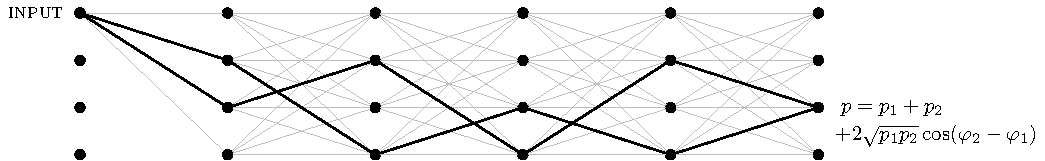
\includegraphics{quantum-info_files/figure-latex/quantum-computation-1} 

}

\caption{Quantum computation.}\label{fig:quantum-computation}
\end{figure}

For quantum computations, we associate with each edge in the graph the probability \emph{amplitude} that the computation follows that edge.
The probability amplitude of a particular path to be followed is the product of amplitudes pertaining to transitions in each step.
The probability amplitude of a particular final state being reached is equal to the sum of the amplitudes along all mutually exclusive paths which connect the initial state with that particular state:
\[
  z = \sum_{\mathrm{all\,paths}\,k} z_k.
\]
The resulting probability, as we have just seen, is the sum of the probabilities pertaining to each computational path \(p_k\) modified by the interference terms:
\[
  \begin{aligned}
    p
    &= |z|^2
  \\&= \sum_{k,j} z_j^\star z_k
  \\&= \sum_k p_k + \sum_{k\ne j} \sqrt{p_k p_j}\cos(\varphi_k-\varphi_j).
  \end{aligned}
\]

\begin{idea}

Quantum computation can be viewed as a complex multi-particle quantum interference involving many computational paths through a computing device.
The art of quantum computation is to shape quantum interference, through a sequence of computational steps, enhancing probabilities of correct outputs and suppressing probabilities of the wrong ones.

\end{idea}

\hypertarget{computational-complexity}{%
\subsection{Computational complexity}\label{computational-complexity}}

Is there a compelling reason why we should care about quantum computation?
It may sound like an extravagant way to compute something that can be computed anyway.
Indeed, your standard laptop, given enough time and memory, can simulate pretty much any physical process.
In principle, it can also simulate any quantum interference and compute everything that quantum computers can compute.
The snag is, this simulation, in general, is very inefficient.
And efficiency does matter, especially if you have to wait more than the age of the Universe for your laptop to stop and deliver an answer!\footnote{The age of the Universe is currently estimated at 13.772 billion years.}

In order to solve a particular problem, computers (classical or quantum) follow a precise set of instructions called an \textbf{algorithm}.
Computer scientists quantify the efficiency of an algorithm according to how rapidly its running time, or the use of memory, increases when it is given ever larger inputs to work on.
An algorithm is said to be \textbf{efficient} if the number of elementary operations taken to execute it increases no faster than a polynomial function of the size of the input.\footnote{Note that the technological progress alone, such as increasing the speed of classical computers, will never turn an inefficient algorithm (exponential scaling) into an efficient one (polynomial scaling). Why?}
We take the input size to be the total number of binary digits (bits) needed to specify the input.
For example, using the algorithm taught in elementary school, one can multiply two \(n\) digit numbers in a time that grows like the number of digits squared, \(n^2\).
In contrast, the fastest-known method for the reverse operation --- factoring an \(n\)-digit integer into prime numbers --- takes a time that grows exponentially, roughly as \(2^n\).
That is considered inefficient.

\begin{center}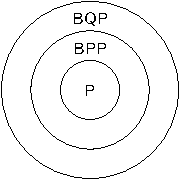
\includegraphics{quantum-info_files/figure-latex/unnamed-chunk-8-1} \end{center}

The class of problems that can be solved by a deterministic computer in polynomial time is represented by the capital letter \texttt{P}, for \emph{polynomial} time.
The class of problems that can be solved in polynomial time by a probabilistic computer is called \texttt{BPP}, for \emph{bounded-error probabilistic polynomial} time.
It is clear that \texttt{BPP} contains \texttt{P}, since a deterministic computation is a special case of a probabilistic computation in which we never consult the source of randomness.
When we run a probabilistic (a.k.a. randomised) computation many times on the same input, we will not get the same answer every time, but the computation is useful if the probability of getting the right answer is high enough.
Finally, the complexity class \texttt{BQP}, for \emph{bounded-error quantum polynomial}, is the class of problems that can be solved in polynomial time by a quantum computer.

\begin{center}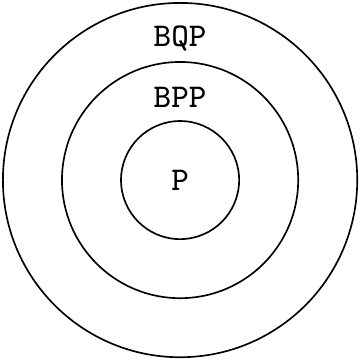
\includegraphics{quantum-info_files/figure-latex/unnamed-chunk-9-1} \end{center}

Since a quantum computer can easily generate random bits and simulate a probabilistic classical computer, \texttt{BQP} certainly contains the class \texttt{BPP}.
Here we are interested in problems that are in \texttt{BQP} but not known to be in \texttt{BPP}.
The most popular example of such a problem is factoring.

A quantum algorithm, discovered by Peter Shor in 1994, can factor \(n\)-digit numbers in a number of steps that grows only as \(n^2\), as opposed to the \(2^n\) that we have classically.\footnote{It must be stressed that not all quantum algorithms are so efficient, in fact many are no faster than their classical counterparts. Which particular problems will lend themselves to quantum speed-ups is an open question.}
Since the intractability of factorisation underpins the security of many methods of encryption, Shor's algorithm was soon hailed as the first `killer application' for quantum computation: something very useful that only a quantum computer could do.
Since then, the hunt has been on for interesting things for quantum computers to do, and at the same time, for the scientific and technological advances that could allow us to build quantum computers.

\hypertarget{outlook}{%
\subsection{Outlook}\label{outlook}}

When the physics of computation was first investigated, starting in the 1960s, one of the main motivations was a fear that quantum-mechanical effects might place fundamental bounds on the accuracy with which physical objects could render the properties of the abstract entities, such as logical variables and operations, that appear in the theory of computation.
It turned out, however, that quantum mechanics itself imposes no significant limits, but does break through some of those that classical physics imposed.
The quantum world has a richness and intricacy that allows new practical technologies, and new kinds of knowledge.
In this course we will merely scratch the surface of the rapidly developing field of quantum computation.
We will concentrate mostly on the fundamental issues and skip many experimental details.
However, it should be mentioned that quantum computing is a serious possibility for future generations of computing devices.
At present it is not clear how and when fully-fledged quantum computers will eventually be built;
but this notwithstanding, the quantum theory of computation already plays a much more fundamental role in the scheme of things than its classical predecessor did.
I believe that anyone who seeks a fundamental understanding of either physics, computation or logic must incorporate its new insights into their world view.

\hypertarget{remarks-and-exercises}{%
\subsection{Remarks and exercises}\label{remarks-and-exercises}}

\hypertarget{section}{%
\subsubsection{}\label{section}}

Back in 1926, Max Born simply postulated the connection between amplitudes and probabilities.
However, it is worth pointing out that he did not get it quite right on his first approach.
In the original paper\footnote{Max Born, ``Zur Quantenmechanik der Stoßvorgänge'', \emph{Zeitschrift für Physik} \textbf{37} (1926), 893--867.} proposing the probability interpretation of the state vector (wavefunction) he wrote:

\begin{quote}
\ldots{} If one translates this result into terms of particles only one interpretation is possible.
\(\Theta_{\eta,\tau,m}(\alpha,\beta,\gamma)\) {[}the wavefunction for the particular problem he is considering{]} gives the probability\(^*\) for the electron arriving from the \(z\) direction to be thrown out into the direction designated by the angles \(\alpha,\beta,\gamma\)\ldots{}

\(^*\) Addition in proof: More careful considerations show that the probability is proportional to the square of the quantity \(\Theta_{\eta,\tau,m}(\alpha,\beta,\gamma)\).
\end{quote}

\hypertarget{section-1}{%
\subsubsection{}\label{section-1}}

Suppose that we modified the Born rule, so that probabilities were given by the absolute values of amplitudes raised to power \(p\) (for \(p\) not necessarily equal to \(2\)).
Then admissible physical evolutions must preserve the normalisation of probability.
Mathematically speaking, they must be isometries of \(p\)-norms.

Recall that the \(p\)-norm of vector \(v\), with components \(v_1, v_2,\ldots, v_n\), is defined as
\[
  \sqrt[\leftroot{1}\uproot{3}p]{|v_1|^p + |v_2|^p + \ldots + |v_n|^p}.
\]
It is clear that any permutation of vector components and multiplication by phase factors (i.e.~unit complex numbers) will leave any \(p\)-norm unchanged.
It turns out that these complex permutations are the \emph{only} isometries, except for \emph{one} special case!
For \(p=2\), the isometries are unitary operations, which form a continuous group; in all other cases we are restricted to discrete permutations.
We do not have to go into details of the proof since we can \emph{see} this result.



\begin{figure}[H]

{\centering 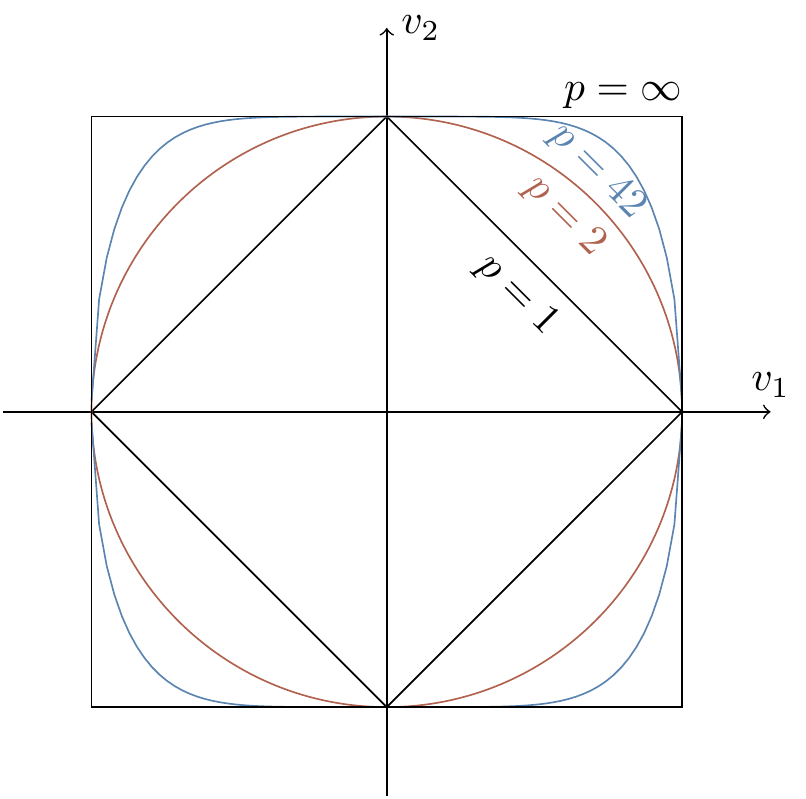
\includegraphics{quantum-info_files/figure-latex/p-norm-unit-spheres-1} 

}

\caption{The unit spheres in the \(p\)-norm for \(p=1,2,42,\infty\).}\label{fig:p-norm-unit-spheres}
\end{figure}

In particular, the image of the unit sphere must be preserved under probability preserving operations.
As we can see in Figure \ref{fig:p-norm-unit-spheres}, the \(2\)-norm is special because of its rotational invariance --- the probability measure picks out no preferred basis in the space of state vectors.
Moreover, it respects unitary operations and does not restrict them in any way.
If the admissible physical evolutions were restricted to discrete symmetries, e.g.~permutations, then there would be no continuity, and no concept of ``time'' as we know it.

\hypertarget{section-2}{%
\subsubsection{}\label{section-2}}

Complex numbers have many applications in physics, however, not until the advent of quantum theory was their ubiquitous and fundamental role in the description of the actual physical world so evident.
Even today, their profound link with probabilities appears to be a rather mysterious connection.
Mathematically speaking, the set of complex numbers is a field. This is an important algebraic structure used in almost all branches of mathematics.
You do not have to know much about algebraic fields to follow these lectures, but still, you should know the basics.
Look them up.

\begin{enumerate}
\def\labelenumi{\alph{enumi}.}
\tightlist
\item
  The set of rational numbers and the set of real numbers are both fields, but the set of integers is not. Why?
\item
  What does it mean to say that the field of complex numbers is \textbf{algebraically closed}?
\item
  Evaluate each of the following quantities:
  \[
   1+e^{-i\pi},
   \quad
   |1+i|,
   \quad
   (1+i)^{42},
   \quad
   \sqrt{i},
   \quad
   2^i,
   \quad
   i^i.
    \]
\item
  Here is a simple proof that \(+1=-1\): \[1=\sqrt{1}=\sqrt{(-1)(-1)}=\sqrt{-1}\sqrt{-1}=i^2=-1.\] What is wrong with it?
\end{enumerate}

\hypertarget{section-3}{%
\subsubsection{}\label{section-3}}

A quantum computer starts calculations in some initial state, then follows \(n\) different computational paths which lead to the final output.
The computational paths are followed with probability amplitudes \(\frac{1}{\sqrt n}e^{i k \varphi}\), where \(\varphi\) is a fixed angle \(0< \varphi <2\pi\) and \(k=0,1,...n-1\).
Show that the probability of generating the output is\footnote{\(1+z+z^2+\ldots + z^n= \frac{1-z^{n+1}}{1-z}\)}
\[
  \frac{1}{n}\left\vert
    \frac{1-e^{i n\varphi}}{1-e^{i\varphi}}
  \right\vert^2
  = \frac{1}{n} \frac{\sin^2 (n\frac{\varphi}{2})}{\sin^2 (\frac{\varphi}{2})}.
\]
for \(0<\varphi<2\pi\), and \(1\) for \(\varphi=0\).
Plot the probability as a function of \(\varphi\).

\hypertarget{section-4}{%
\subsubsection{}\label{section-4}}

Imagine two distant stars, A and B, that emit \emph{identical} photons.
If you point a single detector towards them you will register a click every now and then, but you never know which star the photon came from.
Now prepare two detectors and point them towards the stars.
Assume the photons arrive with the probability amplitudes specified in Figure \ref{fig:photons-from-stars}.
Every now and then you will register a coincidence: the two detectors will fire.

\begin{enumerate}
\def\labelenumi{\alph{enumi}.}
\tightlist
\item
  Calculate the probability of a coincidence.
\item
  Now, assume that \(z\approx \frac{1}{r}e^{i\frac{2r\pi}{\lambda}}\), where \(r\) is the distance between detectors and the stars. How can we use this to measure \(r\)?
\end{enumerate}

\begin{figure}[H]

{\centering 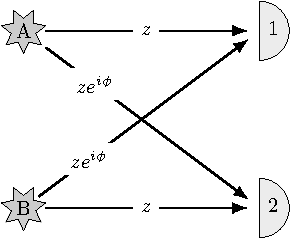
\includegraphics{quantum-info_files/figure-latex/photons-from-stars-1} 

}

\caption{Two photon detectors pointing at two stars, with the probabilities of detection.}\label{fig:photons-from-stars}
\end{figure}

\hypertarget{physics-against-logic}{%
\subsubsection{Physics against logic?}\label{physics-against-logic}}

Now that we have poked our heads into the quantum world, let us see how quantum interference challenges conventional logic and leads to qualitatively different computations.
Consider the following task (which we will return to a few more times in later chapters): design a logic gate that operates on a single bit such that, when it is followed by another, identical, logic gate, the output is \emph{always} the negation of the input.
Let us call this logic gate \textbf{the square root of \(\texttt{NOT}\)}, or \(\sqrt{\texttt{NOT}}\).
A simple check, such as an attempt to construct a truth table, should persuade you that there is no such operation in logic.
It may seem reasonable to argue that since there is no such operation in logic, \(\sqrt{\texttt{NOT}}\) is impossible.
Think again!

Figure \ref{fig:sqrt-not} shows a simple computation, two identical computational steps performed on two states labelled as \(0\) and \(1\), i.e.~on one bit.
An interplay of constructive and destructive interference makes some transitions impossible and the result is the logical \(\texttt{NOT}\).
Thus, quantum theory declares, the square root of \(\texttt{NOT}\) is possible.
And it does exist!
Experimental physicists routinely construct this and many other ``impossible'' gates in their laboratories.
They are the building blocks of a quantum computer.
Quantum theory explains the behaviour of \(\sqrt{\texttt{NOT}}\), hence, reassured by the physical experiments that corroborate this theory, logicians are now entitled to propose a new logical operation \(\sqrt{\texttt{NOT}}\).
Why?
Because a faithful physical model for it exists in nature.

Write a \(2\times 2\) matrix which describes the \(\sqrt{\texttt{NOT}}\) operation.
Is there just one such a matrix?
Suppose you are given a supply of Hadamard and phase gates with tuneable phase settings.
How would you construct the \(\sqrt{\texttt{NOT}}\) gate?



\begin{figure}[H]

{\centering 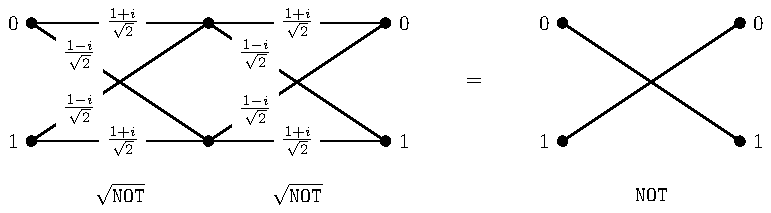
\includegraphics{quantum-info_files/figure-latex/sqrt-not-1} 

}

\caption{A computation that, when repeated, gives exactly \(\texttt{NOT}\). An unlabelled line means that it has probability \(1\), and the lack of a line corresponds to having probability \(0\).}\label{fig:sqrt-not}
\end{figure}

\hypertarget{quantum-bomb-tester}{%
\subsubsection{Quantum bomb tester}\label{quantum-bomb-tester}}

You have been drafted by the government to help in the demining effort in a former war-zone.\footnote{This is a slightly modified version of a bomb testing problem described by Avshalom Elitzur and Lev Vaidman in \emph{Quantum-mechanical interaction-free measurement}, Found. Phys. \textbf{47} (1993), 987-997.}
In particular, retreating forces have left very sensitive bombs in some of the sealed rooms.
The bombs are configured such that if even one photon of light is absorbed by the fuse (i.e.~if someone looks into the room), the bomb will go off.
Each room has an input and output port which can be hooked up to external devices.
An empty room will let light go from the input to the output ports unaffected, whilst a room with a bomb will explode if light is shone into the input port and the bomb absorbs even just one photon --- see Figure \ref{fig:bomb-detecting-scenario}.



\begin{figure}[H]

{\centering 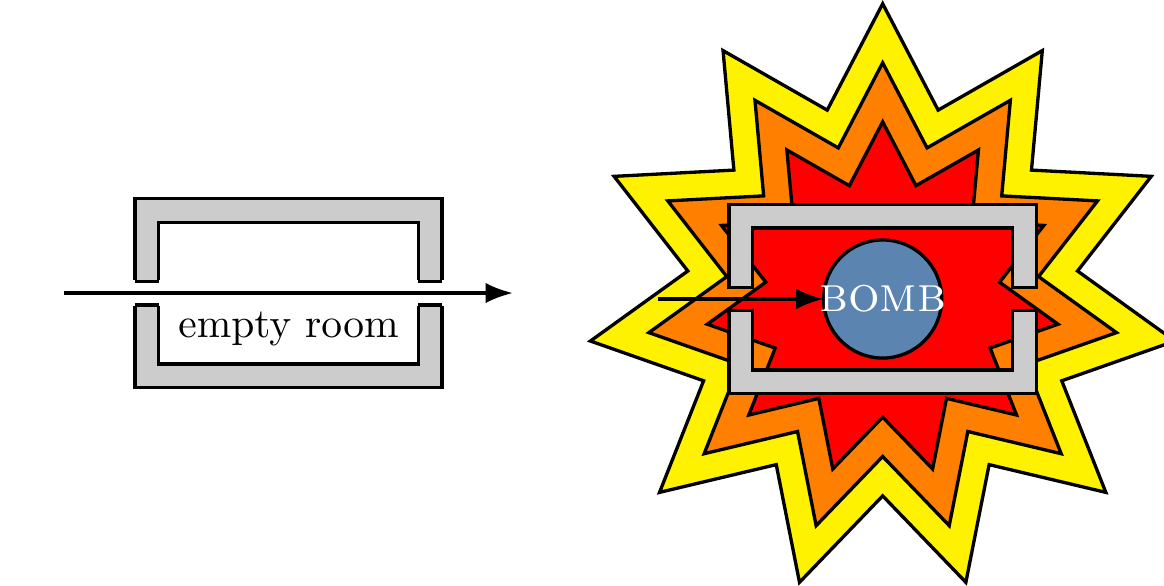
\includegraphics{quantum-info_files/figure-latex/bomb-detecting-scenario-1} 

}

\caption{\emph{Left} --- the passage of a photon through an empty room. \emph{Right} --- the passage of a photon through a room containing a bomb.}\label{fig:bomb-detecting-scenario}
\end{figure}

Your task is to find a way of determining whether a room has a bomb in it without blowing it up, so that specialised (limited and expensive) equipment can be devoted to defusing that particular room.
You would like to know with certainty whether a particular room had a bomb in it.

\begin{enumerate}
\def\labelenumi{\arabic{enumi}.}
\tightlist
\item
  To start with, consider the setup in Figure \ref{fig:mach-zehnder-bomb-tester}, where the input and output ports are hooked up in the lower arm of a Mach-Zehnder interferometer.\footnote{Read about a Mach-Zehnder interferometer in {[}Supplement: Quantum interference revisited (still about beam-splitters){]}.}

  \begin{enumerate}
  \def\labelenumii{\alph{enumii}.}
  \tightlist
  \item
    Assume an empty room.
    Send a photon to input port \(|0\rangle\).
    Which detector, at the output port, will register the photon?
  \item
    Now assume that the room does contain a bomb.
    Again, send a photon to input port \(|0\rangle\).
    Which detector will register the photon and with which probability?
  \item
    Design a scheme that allows you --- at least some of the time --- to decide whether a room has a bomb in it without blowing it up.
    If you iterate the procedure, what is its overall success rate for the detection of a bomb without blowing it up?
  \end{enumerate}
\end{enumerate}

\begin{figure}[H]

{\centering 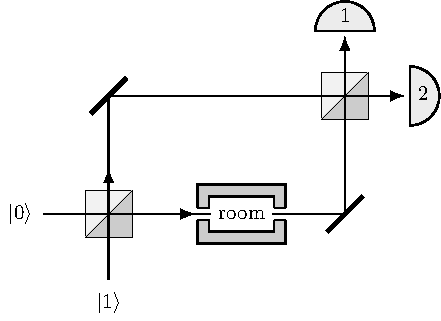
\includegraphics{quantum-info_files/figure-latex/mach-zehnder-bomb-tester-1} 

}

\caption{The Mach-Zehnder interferometer hooked up to the bomb-testing room.}\label{fig:mach-zehnder-bomb-tester}
\end{figure}

\begin{enumerate}
\def\labelenumi{\arabic{enumi}.}
\setcounter{enumi}{1}
\item
  Assume that the two beam splitters in the interferometer are different.
  Say the first beam-splitter reflects incoming light with probability \(r\) and transmits with probability \(t=1-r\), and the second one transmits with probability \(r\) and reflects with probability \(t\).
  Would the new setup improve the overall success rate of the detection of a bomb without blowing it up?
\item
  There exists a scheme, involving many beam-splitters and something called the \textbf{quantum Zeno effect}, such that the success rate for detecting a bomb without blowing it up approaches 100\%.
  Try to work it out, or find a solution on the internet.
\end{enumerate}

\hypertarget{section-5}{%
\subsubsection{}\label{section-5}}

A quantum machine has \(N\) perfectly distinguishable configurations.
What is the maximum number of computational paths connecting a specific input with a specific output after \(k\) steps of the machine?
Suppose you are using your laptop to add together amplitudes pertaining to each of the paths.
As \(k\) and \(N\) increase you may need more time and more memory to complete the task.
How does the execution time and the memory requirements grow with \(k\) and \(N\)?
Will you need more time or more memory or both?

\hypertarget{section-6}{%
\subsubsection{}\label{section-6}}

The classical theory of computation is essentially the theory of the universal Turing machine --- the most popular mathematical model of classical computation.
Its significance relies on the fact that, given a large but finite amount of time, the universal Turing machine is capable of any computation that can be done by any modern classical digital computer, no matter how powerful.
The concept of Turing machines may be modified to incorporate quantum computation, but we will not follow this path.
It is much easier to explain the essence of quantum computation talking about quantum logic gates and quantum Boolean networks or circuits.
The two approaches are computationally equivalent, even though certain theoretical concepts, e.g.~in computational complexity, are easier to formulate precisely using the Turing machine model.
The main advantage of quantum circuits is that they relate far more directly to proposed experimental realisations of quantum computation.

\hypertarget{section-7}{%
\subsubsection{}\label{section-7}}

In computational complexity the basic distinction is between polynomial and exponential algorithms.
Polynomial growth is good and exponential growth is bad, especially if you have to pay for it.
There is an old story about the legendary inventor of chess who asked the Persian king to be paid only by a grain of cereal, doubled on each of the 64 squares of a chess board.
The king placed one grain of rice on the first square, two on the second, four on the third, and he was supposed to keep on doubling until the board was full.
The last square would then have \(2^{63}=9,223,372,036,854,775,808\) grains of rice, more than has been ever harvested on planet Earth, to which we must add the grains of all previous squares, making the total number about twice as large.
If we placed that many grains in an unbroken line we would reach the nearest star Alpha Centauri, our closest celestial neighbour beyond the solar system, about \(4.4\) light-years away.\footnote{One light year (the distance that light travels through a vacuum in one year) is \(9.4607 \times 10^{15}\)m.}
The moral of the story: if whatever you do requires an exponential use of resources, you are in trouble.

\hypertarget{section-8}{%
\subsubsection{}\label{section-8}}

In order to make qualitative distinctions between how different functions grow we will often use the asymptotic big-\(O\) notation.
For example, suppose an algorithm running on input of size \(n\) takes \(a n^2+bn+c\) elementary steps, for some positive constants \(a, b\) and \(c\).
These constants depend mainly on the details of the implementation and the choice of elementary steps.
What we really care about is that, for large \(n\), the whole expression is dominated by its quadratic term.
We then say that the running time of this algorithm grows as \(n^2\), and we write it as \(O(n^2)\), ignoring the less significant terms and the constant coefficients.
More precisely, let \(f(n)\) and \(g(n)\) be functions from positive integers to positive reals.
You may think of \(f(n)\) and \(g(n)\) as the running times of two algorithms on inputs of size \(n\).
We say \(f=O(g)\),\footnote{\(f=O(g)\) is pronounced as ``\(f\) is big-oh of \(g\)''.} which means that \(f\) grows no faster than \(g\), if there is a constant \(c>0\) such that \(f(n)\leqslant c g(n)\) for all sufficiently large values of \(n\).
Essentially, \(f=O(g)\) is a very loose analogue of \(f \leqslant g\).
In addition to the big-\(O\) notation, computer scientists often use \(\Omega\) for lower bounds: \(f=\Omega (g)\) means \(g=O(f)\).
Again, this is a very loose analogue of \(f \geqslant g\).

\begin{enumerate}
\def\labelenumi{\arabic{enumi}.}
\item
  When we say that \(f(n)=O(\log n)\), why don't we have to specify the base of the logarithm?
\item
  Let \(f(n)=5n^3+1000n+50\). Is \(f(n)=O(n^3)\), or \(O(n^4)\), or both?
\item
  Which of the following statements are true?

  \begin{enumerate}
  \def\labelenumii{\alph{enumii}.}
  \tightlist
  \item
    \(n^k=O(2^n)\) for any constant \(k\)
  \item
    \(n!=O(n^n)\)
  \item
    if \(f_1=O(g)\) and \(f_2=O(g)\), then \(f_1+f_2=O(g)\).
  \end{enumerate}
\end{enumerate}

\hypertarget{section-9}{%
\subsubsection{}\label{section-9}}

There exists a randomised algorithm which tests whether a given number \(N\) is prime.\footnote{Primality used to be given as the classic example of a problem in \textsf{BPP} but not \textsf{P}. However, in 2002 a deterministic polynomial time test for primality was proposed by Manindra Agrawal, Neeraj Kayal, and Nitin Saxena. Thus, since 2002, primality has been in \textsf{P}.}
The algorithm always returns \(\texttt{yes}\) when \(N\) is prime, and the probability it returns \(\texttt{yes}\) when \(N\) is not prime is \(\epsilon\), which not greater than a half (independently, each time you run the algorithm).
You run this algorithm (for the same \(N\)) \(r\) times and each time the algorithm returns \(\texttt{yes}\).
What is the probability that \(N\) is not prime?

\hypertarget{section-10}{%
\subsubsection{}\label{section-10}}

Suppose a randomised algorithm solves a decision problem, returning \(\texttt{yes}\) or \(\texttt{no}\) answers.
It gets the answer wrong with a probability not greater than \(\frac12-\delta\), where \(\delta>0\) is a constant.\footnote{This result is known as the \textbf{Chernoff bound}.}.
If we are willing to accept a probability of error no larger than \(\epsilon\), then it suffices to run the computation \(r\) times, where \(r=O(\log 1/\epsilon)\).\}

\begin{center}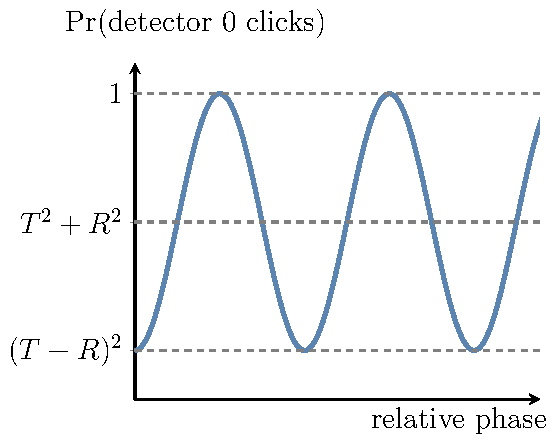
\includegraphics{quantum-info_files/figure-latex/unnamed-chunk-10-1} \end{center}

\begin{enumerate}
\def\labelenumi{\arabic{enumi}.}
\tightlist
\item
  If we perform this computation \(r\) times, how many possible sequences of outcomes are there?
\item
  Give a bound on the probability of any particular sequence with \(w\) wrong answers.
\item
  If we look at the set of \(r\) outcomes, we will determine the final outcome by performing a majority vote.
  This can only go wrong if \(w>r/2\).
  Give an upper bound on the probability of any single sequence that would lead us to the wrong conclusion.
\item
  Using the bound \(1-x\leqslant e^{-x}\), conclude that the probability of our coming to the wrong conclusion is upper bounded by \(e^{-2r\delta^2}\).
\end{enumerate}

\hypertarget{chapter2}{%
\section{Qubits}\label{chapter2}}

\begin{quote}
About quantum bits and quantum circuits, including the ``impossible'' square root of \(\texttt{NOT}\), as well as an introduction to single-qubit unitaries and rotations of the Bloch sphere, and the implications concerning universal gates.
\end{quote}

\hypertarget{composing-quantum-operations}{%
\subsection{Composing quantum operations}\label{composing-quantum-operations}}

In order to understand something in its full complexity it is always good to start with the simplest case.
Let us take a closer look at quantum interference in the simplest possible computing machine: the one that has only two distinguishable configurations --- two quantum states --- which we label as \(|0\rangle\) and \(|1\rangle\).
We prepare the machine in some input state, usually \(|0\rangle\), and let it \textbf{evolve}: the machine undergoes a prescribed sequence of computational steps, each of which induces transitions between the two ``computational states'', \(|0\rangle\) and \(|1\rangle\).
The machine then ends in the output state \(|\psi\rangle=\alpha_0|0\rangle+\alpha_1|1\rangle\), meaning the two outputs, \(|0\rangle\) and \(|1\rangle\), are reached with probability amplitudes \(\alpha_0\) and \(\alpha_1\), respectively.
In the process of computation each computational step \(U\) (also referred to as an \textbf{operation}) sends state \(|k\rangle\) to state \(|l\rangle\), where \(k,l=0,1\), but only with some \textbf{amplitude} \(U_{lk}\).
We write this as
\begin{equation}
  |k\rangle \mapsto \sum_l U_{lk} |l\rangle.
\label{eq:pulsemap}
\end{equation}
(watch out for the order of the indices).

Thus any computational step \(U\) of this machine can be described by a matrix which tabulates all the transition amplitudes:
\[
  U =
  \begin{bmatrix}
    U_{00} & U_{01}
  \\U_{10} & U_{11}
  \end{bmatrix}.
\]
The matrix element \(U_{lk}\) represents the amplitude of transition from state \(|k\rangle\) to state \(|l\rangle\) (again, watch the order of indices).
To be clear, the entries in this matrix are not any random complex numbers: their moduli squared represent transition probabilities, which in turn implies that such matrices must be \textbf{unitary}.\footnote{Recall that matrix \(U\) is called \textbf{unitary} if \[U^\dagger U = UU^\dagger = \operatorname{id}\] where the \textbf{adjoint} or \textbf{Hermitian conjugate} \(U^\dagger\) of any matrix \(U\) with complex entries \(U_{ij}\) is obtained by taking the complex conjugate of every element in the matrix and then interchanging rows and columns (\(U^\dagger_{kl}= U^\star_{lk}\)).}

We can also describe \(U\) by drawing a diagram, which contains exactly the same information as the matrix representation, but just in a different form:

\begin{center}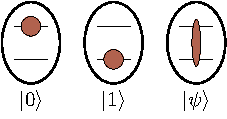
\includegraphics{quantum-info_files/figure-latex/unnamed-chunk-11-1} \end{center}

Now how can we find some quantum interference to study?
Consider two computational steps, \(U\) and \(V\).
What is the amplitude that input \(|k\rangle\) will generate output \(|m\rangle\)?
We have to check all computational paths leading from input \(|k\rangle\) to output \(|m\rangle\) and add the corresponding amplitudes.
For example, as you can see in Figure \ref{fig:composition-of-two-computation-steps}, input \(|0\rangle\) and output \(|1\rangle\) are connected by the two computational paths: \(|0\rangle\mapsto|0\rangle\mapsto|1\rangle\) (amplitude \(V_{10}U_{00}\)) and \(|0\rangle\mapsto|1\rangle\mapsto|1\rangle\) (amplitude \(V_{11}U_{10}\)).
Thus the total amplitude that input \(|0\rangle\) gives output \(|1\rangle\) is the sum \(V_{10}U_{00}+V_{11}U_{10}\), and when we take the modulus squared of this expression we will see the interference term.



\begin{figure}[H]

{\centering 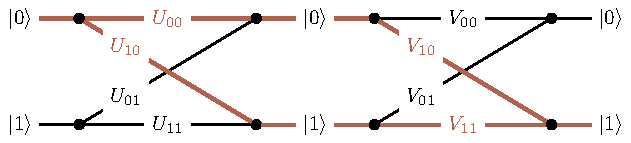
\includegraphics{quantum-info_files/figure-latex/composition-of-two-computation-steps-1} 

}

\caption{The composition of two computational steps, \(U\) and \(V\), with the possible paths from \(|0\rangle\) to \(|1\rangle\) highlighted.}\label{fig:composition-of-two-computation-steps}
\end{figure}

In general, given \(U\) and \(V\)
\[
  \begin{aligned}
    |k\rangle
    &\mapsto
    \sum_l U_{lk}|l\rangle
  \\|l\rangle
    &\mapsto
    \sum_m V_{ml}|m\rangle
  \end{aligned}
\]
we can compose the two operations: we first apply \(U\), and then \(V\), to obtain
\[
  \begin{aligned}
    |k\rangle
    &\mapsto
    \sum_l U_{lk} \left(
      \sum_m V_{ml}|m\rangle
    \right)
  \\&=
    \sum_m \left(
      \sum_l V_{ml}U_{lk}
    \right) |m\rangle
  \\&=
    \sum_m (VU)_{mk} |m\rangle.
  \end{aligned}
\]

If you want to hone your quantum intuition think about it the following way.
The amplitude that input \(|k\rangle\) evolves to \(|m\rangle\) via a specific intermediate state \(|l\rangle\) is given by \(V_{ml}U_{lk}\) (evolutions are independent so the amplitudes are multiplied).
This done, we have to sum over all possible values of \(l\) (the transition can occur in several mutually exclusive ways so the amplitudes are added) to obtain \(\sum_l V_{ml}U_{lk}\).
Thus the matrix multiplication \(VU\) (watch the order of matrices) in one swoop takes care of multiplication and addition of amplitudes corresponding to different computational paths.

\hypertarget{quantum-bits-called-qubits}{%
\subsection{Quantum bits, called ``qubits''}\label{quantum-bits-called-qubits}}

A two-state machine that we have just described in abstract terms is usually realised as a controlled evolution of a two state system, called a quantum bit or a qubit.
For example, state \(|0\rangle\) may be chosen to be the lowest energy state of an atom, the \textbf{ground state}, and state \(|1\rangle\) a higher energy state, the \textbf{excited state}.
Pulses of light of appropriate frequency, duration and intensity can take the atom back and forth between the basis states \(|0\rangle\) and \(|1\rangle\) (implementing logical \(\texttt{NOT}\)).

\begin{center}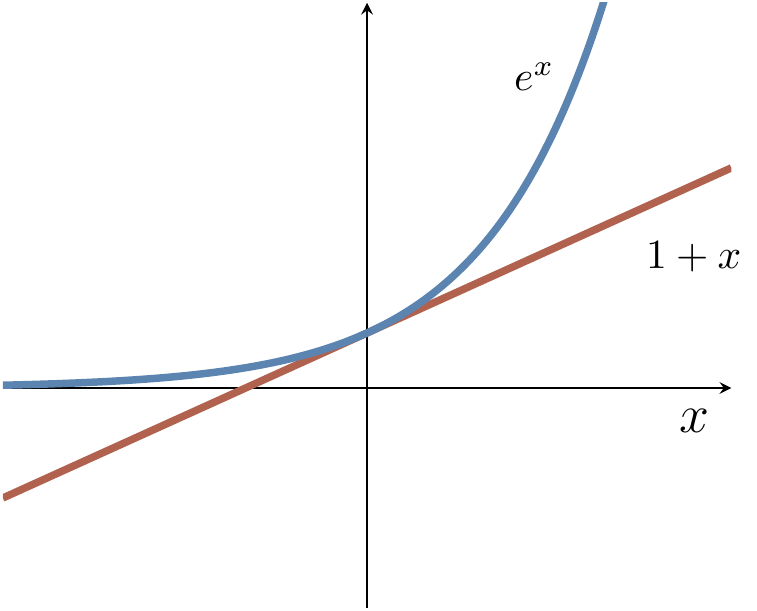
\includegraphics{quantum-info_files/figure-latex/unnamed-chunk-12-1} \end{center}

Some other pulses, say, half the duration or intensity will take the atom into states that have no classical analogue.
Such states are called \textbf{coherent superpositions} of \(|0\rangle\) and \(|1\rangle\), and represent a qubit in state \(|0\rangle\) with some amplitude \(\alpha_0\) and in state \(|1\rangle\) with some other amplitude \(\alpha_1\).
This is conveniently represented by a state vector
\[
    |\psi\rangle =
    \alpha_0|0\rangle + \alpha_1|1\rangle
    \leftrightarrow
    \begin{bmatrix}
      \alpha_0
    \\\alpha_1
    \end{bmatrix}
\]

\begin{center}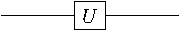
\includegraphics{quantum-info_files/figure-latex/unnamed-chunk-13-1} \end{center}

\begin{idea}

A \textbf{qubit} is a quantum system in which the Boolean states \(0\) and \(1\) are represented by a prescribed pair of normalised and mutually orthogonal quantum states labelled as \(\{|0\rangle,|1\rangle\}\).
The two states form a so-called \textbf{computational} (or \textbf{standard}) basis, and so any other state of an isolated qubit can be written as a coherent superposition
\[
  |\psi\rangle = \alpha_0|0\rangle + \alpha_1|1\rangle
\]
for some \(\alpha_0\) and \(\alpha_1\) such that \(|\alpha_0|^2 + |\alpha_1|^2 = 1\).

In practice, a qubit is typically a microscopic system, such as an atom, a nuclear spin, or a polarised photon.

\end{idea}

As we have already mentioned, any\footnote{ Here we are talking about \emph{isolated} systems. As you will soon learn, a larger class of physically admissible operations is described by completely positive maps. It may sound awfully complicated but, as you will soon see, it is actually very simple.} computational step, that is, any physically admissible operation \(U\) on a qubit, is described by a \((2\times 2)\) unitary matrix \(U\).
It modifies the state of the qubit as
\[
  |\psi\rangle
  \mapsto
  |\psi'\rangle
  =
  U|\psi\rangle
\]
which we can write explicitly as
\[
  \begin{bmatrix}
    \alpha'_0
  \\\alpha'_1
  \end{bmatrix}
  =
  \begin{bmatrix}
    U_{00} & U_{01}
  \\U_{10} & U_{11}
  \end{bmatrix}
  \begin{bmatrix}
    \alpha_0
  \\\alpha_1
  \end{bmatrix}
\]
That is, the operation \(U\) turns the state \(|\psi\rangle\), with components \(\alpha_k\), into the state \(|\psi'\rangle=U|\psi\rangle\), with components \(\alpha'_l= \sum_k U_{lk}\alpha_k\).

\hypertarget{quantum-gates-and-circuits}{%
\subsection{Quantum gates and circuits}\label{quantum-gates-and-circuits}}

Atoms, trapped ions, molecules, nuclear spins and many other quantum objects, which we call qubits, can be used to implement simple quantum interference, and hence simple quantum computation.
There is no need to learn about physics behind these diverse technologies if all you want is to understand the basics of quantum computation.
We may now conveniently forget about any specific experimental realisation of a qubit and just remember that any manipulations on qubits have to be performed by physically admissible operations, and that such operations are represented by unitary transformations.

\begin{idea}

A \textbf{quantum (logic) gate} is a device which performs a fixed unitary operation on selected qubits in a fixed period of time, and a \textbf{quantum circuit} is a device consisting of quantum logic gates whose computational steps are synchronised in time.
The \textbf{sizes} of the circuit is the number of gates it contains.

\end{idea}

Some unitary \(U\) acting on a single qubit is represented diagrammatically as

\begin{center}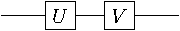
\includegraphics{quantum-info_files/figure-latex/unnamed-chunk-14-1} \end{center}

This diagram should be read from left to right.
The horizontal line represents a qubit that is inertly carried from one quantum operation to another.
We often call this line a \textbf{quantum wire}.
The wire may describe translation in space (e.g.~atoms travelling through cavities) or translation in time (e.g.~a sequence of operations performed on a trapped ion).
A sequence of two gates acting on the same qubit, say \(U\) followed by \(V\), is represented by

\begin{center}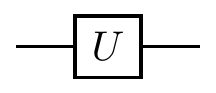
\includegraphics{quantum-info_files/figure-latex/unnamed-chunk-15-1} \end{center}

and is described by the matrix product \(VU\) (note the order in which we multiply the matrices).

\hypertarget{single-qubit-interference}{%
\subsection{Single qubit interference}\label{single-qubit-interference}}

Let me now describe what is probably the most important sequence of operations performed on a single qubit, namely a generic \textbf{single qubit interference}.
It is typically constructed as a sequence of three elementary operations:

\begin{enumerate}
\def\labelenumi{\arabic{enumi}.}
\tightlist
\item
  the Hadamard gate
\item
  a phase shift gate
\item
  the Hadamard gate again.
\end{enumerate}

We represent it graphically as

\begin{center}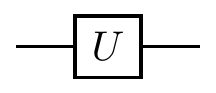
\includegraphics{quantum-info_files/figure-latex/unnamed-chunk-16-1} \end{center}

\begin{idea}

\begin{longtable}[]{@{}cc@{}}
\toprule
\begin{minipage}[b]{(\columnwidth - 1\tabcolsep) * \real{0.62}}\centering
Hadamard\strut
\end{minipage} & \begin{minipage}[b]{(\columnwidth - 1\tabcolsep) * \real{0.38}}\centering
Phase\strut
\end{minipage}\tabularnewline
\midrule
\endhead
\begin{minipage}[t]{(\columnwidth - 1\tabcolsep) * \real{0.62}}\centering
\(H=\frac{1}{\sqrt2}\begin{bmatrix}1&1\\1&-1\end{bmatrix}\)\strut
\end{minipage} & \begin{minipage}[t]{(\columnwidth - 1\tabcolsep) * \real{0.38}}\centering
\(P_\varphi=\begin{bmatrix}1&0\\0&e^{i\varphi}\end{bmatrix}\)\strut
\end{minipage}\tabularnewline
\begin{minipage}[t]{(\columnwidth - 1\tabcolsep) * \real{0.62}}\centering
\(\begin{array}{lcr}|0\rangle&\mapsto&\frac1{\sqrt{2}}(|0\rangle+|1\rangle)\\|1\rangle&\mapsto&\frac1{\sqrt{2}}(|0\rangle-|1\rangle)\end{array}\)\strut
\end{minipage} & \begin{minipage}[t]{(\columnwidth - 1\tabcolsep) * \real{0.38}}\centering
\(\begin{array}{lcr}|0\rangle&\mapsto&|0\rangle\\|1\rangle&\mapsto&e^{i\varphi}|1\rangle\end{array}\)\strut
\end{minipage}\tabularnewline
\bottomrule
\end{longtable}

\end{idea}

You will see it over and over again, for it is quantum interference that gives quantum computation additional capabilities.
The product of the three matrices \(HP_\varphi H\) describes the action of the whole circuit: it gives the transition amplitudes between states \(|0\rangle\) and \(|1\rangle\) at the input and the output as
\[
  e^{i\frac{\varphi}{2}}
  \begin{bmatrix}
    \cos\varphi/2 & -i\sin\varphi/2
  \\-i\sin\varphi/2 & \cos\varphi/2
  \end{bmatrix}
  =
  \frac{1}{\sqrt 2}
  \begin{bmatrix}
    1 & 1
  \\1 & -1
  \end{bmatrix}
  \begin{bmatrix}
    1 & 0
  \\0 & e^{i\varphi}
  \end{bmatrix}
  \frac{1}{\sqrt 2}
  \begin{bmatrix}
    1 & 1
  \\1 & -1
  \end{bmatrix}
\]

Given that our input state is almost always \(|0\rangle\), it is sometimes much easier and more instructive to step through the execution of this circuit and follow the evolving state.
The interference circuit effects the following sequence of transformations:\footnote{We ignore the global phase factor \(e^{i\frac{\varphi}{2}}\).}
\[
  \begin{aligned}
    |0\rangle
    &\overset{H}{\longmapsto}
    \frac{1}{\sqrt2} \left(
      |0\rangle+|1\rangle
    \right)
  \\&\overset{P_\phi}{\longmapsto}
    \frac{1}{\sqrt2} \left(
      |0\rangle+e^{i\phi}|1\rangle
    \right)
  \\&\overset{H}{\longmapsto}
    \cos\frac{\phi}{2}|0\rangle - i\sin\frac{\phi}{2}|1\rangle.
  \end{aligned}
\]
The first Hadamard gate prepares an equally weighted superposition of \(|0\rangle\) and \(|1\rangle\) and the second one closes the interference by bringing the interfering paths together.
The phase shift \(\varphi\) effectively controls the evolution and determines the output.
The probabilities of finding the qubit in state \(|0\rangle\) or \(|1\rangle\) at the output are, respectively,
\[
  \begin{aligned}
    \Pr(0) &= \cos^2\frac{\phi}{2}
  \\\Pr(1) &= \sin^2\frac{\phi}{2}.
  \end{aligned}
\]
This simple quantum process contains, in a nutshell, the essential ingredients of quantum computation.
This sequence (Hadamard -- phase shift -- Hadamard) will appear over and over again.
It reflects a natural progression of quantum computation: first we prepare different computational paths, then we evaluate a function which effectively introduces phase shifts into different computational paths, then we bring the computational paths together at the output.

\hypertarget{the-square-root-of-not}{%
\subsection{The square root of NOT}\label{the-square-root-of-not}}

Now that we have poked our heads into the quantum world, let us see how quantum interference challenges conventional logic.
Consider a following task: design a logic gate that operates on a single bit and such that when it is followed by another, identical, logic gate the output is always the negation of the input.
Let us call this logic gate \textbf{the square root of \(\texttt{NOT}\)}, or \(\sqrt{\texttt{NOT}}\).

\begin{center}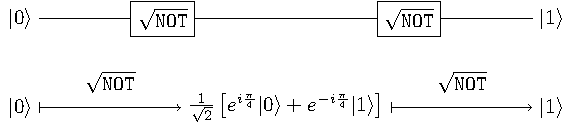
\includegraphics{quantum-info_files/figure-latex/unnamed-chunk-17-1} \end{center}

A simple check, such as an attempt to construct a truth table, should persuade you that there is no such operation in logic.
It may seem reasonable to argue that since there is no such operation in logic, \(\sqrt{\texttt{NOT}}\) is impossible.
But it does exist!
Experimental physicists routinely construct such ``impossible'' gates in their laboratories.
It is a physically admissible operation described by the unitary matrix\footnote{There are infinitely many unitary operations that act as the square root of \(\texttt{NOT}\).}
\[
  \sqrt{\texttt{NOT}}
  =
  \frac12
  \begin{bmatrix}
    1+i & 1-i
  \\1-i&1+i
  \end{bmatrix}
  =
  \frac1{\sqrt2}
  \begin{bmatrix}
    e^{i\frac{\pi}{4}} & e^{-i\frac{\pi}{4}}
  \\e^{-i\frac{\pi}{4}} & e^{i\frac{\pi}{4}}
  \end{bmatrix}.
\]
Indeed,
\[
  \frac12
  \begin{bmatrix}
    1+i & 1-i
  \\1-i & 1+i
  \end{bmatrix}
  \frac12
  \begin{bmatrix}
    1+i & 1-i
  \\1-i & 1+i
  \end{bmatrix}
  =
  \begin{bmatrix}
    0&1
  \\1&0
  \end{bmatrix}.
\]

We could also step through the circuit diagram and follow the evolution of the state vector:

\begin{center}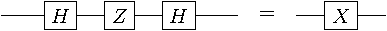
\includegraphics{quantum-info_files/figure-latex/unnamed-chunk-18-1} \end{center}

Or, if you prefer to work with column vectors and matrices, you can write the two consecutive application of \(\sqrt{\texttt{NOT}}\) to state \(|0\rangle\) as
\[
  \begin{bmatrix}0\\1\end{bmatrix}
  \,\longleftarrow\!\!\!\vert\,\,
  \frac{1}{\sqrt 2}
  \begin{bmatrix}
    e^{i\frac{\pi}{4}}
  \\e^{-i\frac{\pi}{4}}
  \end{bmatrix}
  \,\longleftarrow\!\!\!\vert\,\,
  \begin{bmatrix}1\\0\end{bmatrix}
\]
(following a well established convention, the above should be read from \emph{right to left})\footnote{Just remember that circuits diagrams are read from \emph{left to right}, and vector and matrix operations go from \emph{right to left}.}, where each \(\longleftarrow\!\!\!\vert\) denotes multiplication by \(\frac1{\sqrt2}\begin{bmatrix}e^{i\frac{\pi}{4}} & e^{-i\frac{\pi}{4}}\\e^{-i\frac{\pi}{4}} & e^{i\frac{\pi}{4}}\end{bmatrix}\).

One way or another, quantum theory explains the behaviour of \(\sqrt{\texttt{NOT}}\), and so, reassured by the physical experiments\footnote{We discuss this in more detail in {[}Appendix: Physics against logic, via beamsplitters{]}.} that corroborate this theory, logicians are now entitled to propose a new logical operation \(\sqrt{\texttt{NOT}}\).
Why?
Because a faithful physical model for it exists in nature!

\hypertarget{phase-gates-galore}{%
\subsection{Phase gates galore}\label{phase-gates-galore}}

As well as the generic phase gate \(P_\varphi\), let us mention three specific phase gates that will frequently pop up (two of which have rather confusing names, at first glance!).

\begin{idea}

\begin{longtable}[]{@{}cccc@{}}
\toprule
\begin{minipage}[b]{(\columnwidth - 3\tabcolsep) * \real{0.27}}\centering
Generic phase\strut
\end{minipage} & \begin{minipage}[b]{(\columnwidth - 3\tabcolsep) * \real{0.20}}\centering
Phase-flip\strut
\end{minipage} & \begin{minipage}[b]{(\columnwidth - 3\tabcolsep) * \real{0.27}}\centering
\(\pi/4\)-phase\strut
\end{minipage} & \begin{minipage}[b]{(\columnwidth - 3\tabcolsep) * \real{0.27}}\centering
\(\pi/8\)-phase\strut
\end{minipage}\tabularnewline
\midrule
\endhead
\begin{minipage}[t]{(\columnwidth - 3\tabcolsep) * \real{0.27}}\centering
\(P_\varphi=\begin{bmatrix}1&0\\0&e^{i\varphi}\end{bmatrix}\)\strut
\end{minipage} & \begin{minipage}[t]{(\columnwidth - 3\tabcolsep) * \real{0.20}}\centering
\(Z=\begin{bmatrix}1&0\\0&-1\end{bmatrix}\)\strut
\end{minipage} & \begin{minipage}[t]{(\columnwidth - 3\tabcolsep) * \real{0.27}}\centering
\(S=\begin{bmatrix}1&0\\0&i\end{bmatrix}\)\strut
\end{minipage} & \begin{minipage}[t]{(\columnwidth - 3\tabcolsep) * \real{0.27}}\centering
\(T=\begin{bmatrix}1&0\\0&e^{i\frac{\pi}{4}}\end{bmatrix}\)\strut
\end{minipage}\tabularnewline
\bottomrule
\end{longtable}

\end{idea}

Note that the phase gate \(P_\varphi\) is only defined up to a global phase factor\footnote{In general, states differing only by a global phase are physically indistinguishable, and so it is physical experimentation that leads us to this mathematical choice of only defining things up to a global phase.}, and so we can write its matrix either as
\[
  P_\varphi =
  \begin{bmatrix}
    1 & 0
  \\0 & e^{i\varphi}
  \end{bmatrix}
\]
or as
\[
  P_\varphi =
  \begin{bmatrix}
    e^{-i\frac{\varphi}{2}} & 0
  \\0 & e^{i\frac{\varphi}{2}}
  \end{bmatrix}
\]
The first version is more common in the quantum information science community, but the second one is sometimes more convenient to use, as it has determinant \(1\), and hence belongs to the group \(\mathrm{SU}(2)\).
We will occasionally switch to the \(\mathrm{SU}(2)\) version of a phase gates, and this is where the \(\pi/4\)-phase and \(\pi/8\)-phase gates get their names, since their \(\mathrm{SU}(2)\) versions have \(e^{\mp i\pi/4}\) and \(e^{\mp i\pi/8}\) (respectively) on the diagonal.

The remaining gate (\(Z\)) is arguably the most important specific phase gate, since it is one of the \textbf{Pauli operators}, which we will now discuss.

\hypertarget{pauli-operators}{%
\subsection{Pauli operators}\label{pauli-operators}}

Adding to our collection of common single-qubit gates, we now look at the three \textbf{Pauli operators}\footnote{We use the standard basis \(\{|0\rangle,|1\rangle\}\) most of the time, and so often refer to operators as matrices.} \(\sigma_x\), \(\sigma_y\), and \(\sigma_z\), also denoted by \(X\), \(Y\), and \(Z\) (respectively).
These three operators, combined with the identity, satisfy a lot of nice formal properties, which we shall examine briefly here, and then return to in more detail in \protect\hyperlink{chapter3}{Chapter 3}.

\begin{idea}

\begin{longtable}[]{@{}cccc@{}}
\toprule
\begin{minipage}[b]{(\columnwidth - 3\tabcolsep) * \real{0.20}}\centering
Identity\strut
\end{minipage} & \begin{minipage}[b]{(\columnwidth - 3\tabcolsep) * \real{0.20}}\centering
Bit-flip\strut
\end{minipage} & \begin{minipage}[b]{(\columnwidth - 3\tabcolsep) * \real{0.35}}\centering
Bit-phase-flip\strut
\end{minipage} & \begin{minipage}[b]{(\columnwidth - 3\tabcolsep) * \real{0.25}}\centering
Phase-flip\strut
\end{minipage}\tabularnewline
\midrule
\endhead
\begin{minipage}[t]{(\columnwidth - 3\tabcolsep) * \real{0.20}}\centering
\(\operatorname{id}=\begin{bmatrix}1&0\\0&1\end{bmatrix}\)\strut
\end{minipage} & \begin{minipage}[t]{(\columnwidth - 3\tabcolsep) * \real{0.20}}\centering
\(X=\begin{bmatrix}0&1\\1&0\end{bmatrix}\)\strut
\end{minipage} & \begin{minipage}[t]{(\columnwidth - 3\tabcolsep) * \real{0.35}}\centering
\(Y=\begin{bmatrix}0&-i\\i&0\end{bmatrix}\)\strut
\end{minipage} & \begin{minipage}[t]{(\columnwidth - 3\tabcolsep) * \real{0.25}}\centering
\(Z=\begin{bmatrix}1&0\\1&-1\end{bmatrix}\)\strut
\end{minipage}\tabularnewline
\bottomrule
\end{longtable}

\end{idea}

The identity is just a quantum wire, and we have already seen the \(X\) and \(Z\) gates in \protect\hyperlink{phase-gates-galore}{Phase gates galore}, as the bit-flip and phase-flip (respectively).
Note that, of these latter two, only the \(X\) gate has a classical analogue (as the logical \(\texttt{NOT}\) operator).
The remaining gate, the \(Y\) operator, describes the combined effect of both the bit- and the phase-flip: \(ZX=iY\).

In fact, this is just one of the equations that the Pauli matrices satisfy.
The Pauli matrices are unitary and Hermitian, they square to the identity, and they anti-commute.
By this last point, we mean that
\[
  \begin{aligned}
    XY+YX&=0,
  \\XZ+ZX&=0,
  \\YZ+ZY&=0.
  \end{aligned}
\]
As already mentioned, they satisfy \(ZX=iY\), but also any cyclic permutation of this equation.

These operators are also called \textbf{sigma matrices}, or \textbf{Pauli spin matrices}.
They are so ubiquitous in quantum physics that they should certainly be memorised.

\hypertarget{from-bit-flips-to-phase-flips-and-back-again}{%
\subsection{From bit-flips to phase-flips, and back again}\label{from-bit-flips-to-phase-flips-and-back-again}}

The Pauli \(Z\) gate is a special case of a phase gate \(P_\varphi\) with \(\varphi=\pi\).
When we insert it into the interference circuit we obtain

\begin{center}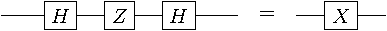
\includegraphics{quantum-info_files/figure-latex/unnamed-chunk-19-1} \end{center}

If you wish to verify this, write the Hadamard gate as \(H = (X+Z)/\sqrt{2}\) and use the properties of the Pauli operators.\footnote{\(\begin{aligned}HXH &= Z\\HZH &= X\\HYH &= -Y\end{aligned}\)}
So the Hadamard gate turns phase-flips into bit-flips, but it also turns bit-flips into phase-flips:

\begin{center}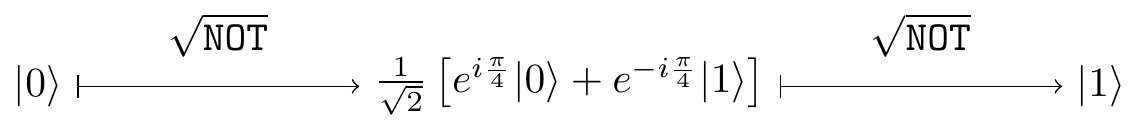
\includegraphics{quantum-info_files/figure-latex/unnamed-chunk-20-1} \end{center}

Let us also add, for completeness, that \(HYH=-Y\).
You will see these identities again and again, especially when we discuss quantum error corrections.\footnote{Unitaries, such as \(H\), that take the three Pauli operators to the Pauli operators via conjugation form the so-called \textbf{Clifford group}, which we will meet later on. Which phase gate is in the Clifford group of a single qubit?}

\hypertarget{any-unitary-operation-on-a-single-qubit}{%
\subsection{Any unitary operation on a single qubit}\label{any-unitary-operation-on-a-single-qubit}}

There are infinitely many unitary operations that can be performed on a single qubit.
In general, any complex \((n\times n)\) matrix has \(n^2\) complex entries, and can thus be specified by \(2n^2\) real independent parameters.
The unitarity constraint removes \(n^2\) of these, and so any unitary \((n\times n)\) matrix has \(n^2\) real independent parameters.
In particular, we need \emph{four} real parameters to specify a \((2\times 2)\) unitary matrix.
If we are prepared to ignore global phase factors (which we are) then there are only three real parameters left.
So, with this in mind, can we construct and implement any unitary on a single qubit in some simple way?

\emph{Yes, we can.}

Any unitary operation on a qubit (up to an overall multiplicative phase factor) can be implemented by a circuit containing just two Hadamards and three phase gates, with adjustable phase settings, as in Figure \ref{fig:universal-circuit-for-2-by-2}.



\begin{figure}[H]

{\centering 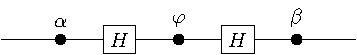
\includegraphics{quantum-info_files/figure-latex/universal-circuit-for-2-by-2-1} 

}

\caption{The universal circuit for unitary \((2\times2)\) matrices.}\label{fig:universal-circuit-for-2-by-2}
\end{figure}

If we multiply the matrices corresponding to each gate in the network (remember that the order of matrix multiplication is reversed) we obtain
\[
  U(\alpha,\beta,\gamma)
  =\begin{bmatrix}
    e^{-i\left(\frac{\alpha+\beta}{2}\right)}\cos\varphi/2
    & -ie^{i\left(\frac{\alpha-\beta}{2}\right)}\sin\varphi/2
  \\-ie^{-i\left(\frac{\alpha-\beta}{2}\right)}\sin\varphi/2
    & e^{i\left(\frac{\alpha+\beta}{2}\right)}\cos\varphi/2
  \end{bmatrix}.
\]
Any \((2\times 2)\) unitary matrix (up to global phase) can be expressed in this form using the three independent real parameters, \(\alpha\), \(\beta,\) and \(\varphi\), which take values in \([0,2\pi]\).
In order to see that this construction does what it claims, let us explore an intriguing mathematical connection between single qubit unitaries and rotations in three dimensions.

\hypertarget{the-bloch-sphere}{%
\subsection{The Bloch sphere}\label{the-bloch-sphere}}

Unitary operations on a single qubit form a group.
More precisely, the set of all \((2\times 2)\) unitary matrices forms a non-abelian group under the matrix multiplication, denoted by \(\mathrm{U}(2)\).
It turns out that compositions of single qubit unitaries behave pretty much the same as compositions of rotations in three dimensions.
Technically speaking, \(\mathrm{U}(2)/\mathrm{U}(1)\cong \mathrm{SO}(3)\).\footnote{Note that \(\mathrm{U}(1)\cong\mathbb{C}^\times\), where \(\mathbb{C}^\times\) is the multiplicative group of unit elements of the complex numbers, i.e.~the set \(\mathbb{C}\setminus\{0\}\) with the group operation given by multiplication.}
That is, \((2\times 2)\) unitaries, up to global phase, form a group which is isomorphic to the group of rotations in three dimensions, denoted by \(\mathrm{SO}(3)\).
This isomorphism helps to visualise the actions of single qubit gates.

There are many ways to introduce this isomorphism.
Here we will first show how to represent single-qubit state vectors in terms of Euclidean vectors in three dimensions, and then relate unitary operations on state vectors to rotations in this Euclidean space.

Any single qubit state can be written as \(|\psi\rangle=\alpha|0\rangle+\beta|1\rangle\), constrained by the relation \(|\alpha|^2+|\beta|^2=1\).
This suggests a more natural parametrisation as\footnote{There is a good reason to use \(\theta/2\) instead of \(\theta\), which we will explain later on.}
\[
  |\psi\rangle =
  \cos\frac{\theta}{2}e^{i\varphi_0}|0\rangle
  + \sin\frac{\theta}{2}e^{i\varphi_1}|1\rangle.
\]
We can then factor out a global phase:
\[
  |\psi\rangle =
  e^{i\varphi_0}\left(
    \cos\frac{\theta}{2}|0\rangle + \sin\frac{\theta}{2}e^{i\varphi}|1\rangle
  \right),
\]
and even remove it completely, since states that are identical up to a global phase are physically indistinguishable.

The parametrisation in terms of \(\theta\) and \(\varphi\) should remind you of spherical polar coordinates for the surface of a sphere.



\begin{figure}[H]

{\centering 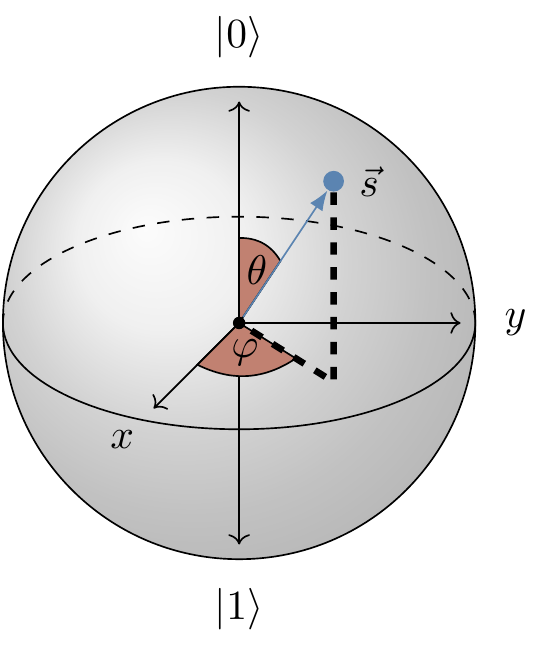
\includegraphics{quantum-info_files/figure-latex/bloch-sphere-1} 

}

\caption{The Bloch sphere, with the point \(\vec{s}\) corresponding to \(|\psi\rangle\) marked.}\label{fig:bloch-sphere}
\end{figure}

We call this sphere the \textbf{Bloch sphere}, and the unit vector \({\vec s}\) defined by \(\theta\) and \(\varphi\) the \textbf{Bloch vector}.\footnote{We will revisit this construction again in more detail, and from a slightly different point of view, in \protect\hyperlink{chapter3}{Chapter 3}.}
This is a very useful way to visualise quantum states of a single qubit and unitary operations that we perform on it.
Any unitary action on the state vector will induce a rotation of the corresponding Bloch vector.
But what kind of rotation?

Note that any two orthogonal state vectors appear on the Bloch sphere as two Bloch vectors pointing in opposite directions.
Now, the two eigenvectors of a single-qubit unitary \(U\) must be orthogonal, and thus define an axis running through the centre of the Bloch sphere.
This is the axis about which the Bloch vector is rotated when \(U\) acts on the corresponding state vector.
The rotation angle \(\alpha\) is given by the eigenvalues of \(U\), which, up to a global phase factor, are of the form \(e^{\mp i\alpha/2}\).

It is instructive to work out few simple cases and get a feel for the rotations corresponding to the most common unitaries.
For example, it is easy to check that a phase gate \(P_\alpha\) acts by
\[
  \cos\frac{\theta}{2}|0\rangle + e^{i\varphi}\sin\frac{\theta}{2}|1\rangle
  \longmapsto
  \cos\frac{\theta}{2}|0\rangle + e^{i(\varphi+\alpha)}\sin\frac{\theta}{2}|1\rangle.
\]
The azimuthal angle changes from \(\varphi\) to \(\varphi+\alpha\), and so the Bloch sphere is rotated anticlockwise by \(\alpha\) about the \(z\)-axis.
The Bloch vectors corresponding to the two eigenvectors of \(P_\alpha\), namely \(|0\rangle\) and \(|1\rangle\), define the axis of the rotation.



\begin{figure}[H]

{\centering 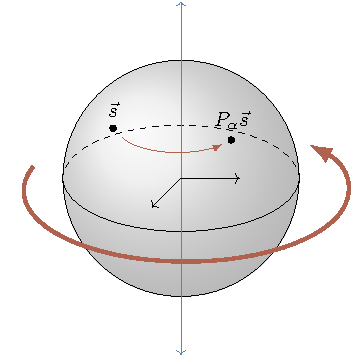
\includegraphics{quantum-info_files/figure-latex/bloch-sphere-rotation-1} 

}

\caption{Phase gates \(P_\alpha\) represent rotations of the Bloch sphere around the \(z\)-axis.}\label{fig:bloch-sphere-rotation}
\end{figure}

As previously mentioned, the Pauli operator \(Z=\sigma_z\) is a special case of a phase gate, and represents rotation by \({180}^{\circ}\) (that is, \(\pi\) radians), about the \(z\)-axis.
You can also verify that \(X=\sigma_x\), with eigenvectors \({(|0\rangle\pm|1\rangle)/\sqrt{2}}\), represents rotation by \({180}^{\circ}\) about the \(x\)-axis, and \(Y=\sigma_y\), with eigenvectors \({(|0\rangle\pm i|1\rangle)/\sqrt{2}}\), represents rotation by \({180}^{\circ}\) about the \(y\)-axis.

How about the Hadamard gate?
Like the Pauli operators, it squares to the identity (\(H^2=\operatorname{id}\)), which implies that its eigenvalues are \(\pm 1\).
Thus it will correspond to a rotation by \({180}^{\circ}\).
But about which axis?
This time, rather than finding eigenvectors of \(H\), we notice that \(HXH=Z\) and \(HZH=X\), thus \(H\) must swap \(x\)- and \(z\)-axes, turning rotations about the \(z\)-axis into rotations about the \(x\)-axis, and vice versa.
The Hadamard gate must then represent rotation by \({180}^{\circ}\) about the diagonal \((x+z)\)-axis.
You may also notice that, after this rotation, the \(y\)-axis points in the opposite direction, which seems to be related to another identity: \(HYH=-Y\).
This is not a coincidence.

One can show\footnote{Again, see \protect\hyperlink{chapter3}{Chapter 3}.} that the effect of the rotation represented by unitary \(U\) on the Bloch vector with components \(s_x\), \(s_y\), \(s_z\) is summarised in the formula
\[
  U (s_x X + s_y Y + s_z Z) U^\dagger
  = s'_x X+ s'_y Y + s'_z Z,
\]
where \(s'_x\), \(s'_y\), and \(s'_z\) are the components of the rotated Bloch vector.

\hypertarget{composition-of-rotations}{%
\subsection{Composition of rotations}\label{composition-of-rotations}}

We are now in a position understand the circuit in Figure \ref{fig:universal-circuit-for-2-by-2} in geometric terms.
Recall that \emph{any} rotation in the Euclidean space can be performed as a sequence of three rotations: one about the \(z\)-axis, one about the \(x\)-axis, and one more about \(z\)-axis.
The circuit does exactly this:

\begin{center}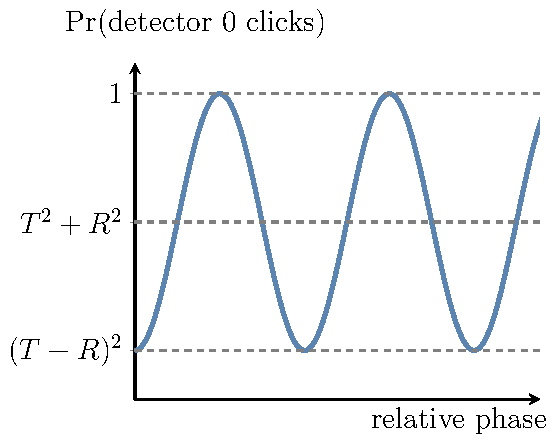
\includegraphics{quantum-info_files/figure-latex/unnamed-chunk-21-1} \end{center}

The first phase gate effects rotation by \(\alpha\) about the \(z\)-axis, the second phase gate is sandwiched between the two Hadamard gates, and these three gates together effect rotation by \(\varphi\) about the \(x\)-axis, and, finally, the third phase gates effects rotation by \(\beta\) about the \(z\)-axis.
So we can implement any unitary \(U\) by choosing the three phase shifts, \(\alpha\), \(\varphi\), and \(\beta\), which are known as the three \textbf{Euler's angles}.

\hypertarget{a-finite-set-of-universal-gates}{%
\subsection{A finite set of universal gates}\label{a-finite-set-of-universal-gates}}

The Hadamard gate and the phase gates, with adjustable phases, allow us to implement an arbitrary single-qubit unitary \emph{exactly}.
The tacit assumption here is that we have here \emph{infinitely many} phase gates: one gate for each phase.
In fact, we can pick just one phase gate, namely any phase gate \(P_\alpha\) with the phase \(\alpha\) that is incommensurate\footnote{That is, there do \emph{not} exist any \(m,n\in\mathbb{Z}\) such that \(m\alpha=n\pi\). For example, it suffices to take \(\alpha\) to be rational.} with \(\pi\).
It is clear that repeated iteration of \(P_\alpha\) can be used to approximate any other phase gate to arbitrary accuracy: indeed, rotate the Bloch sphere by \(\alpha\) about the \(z\)-axis sufficiently many times and you end up as close as you please to any other rotation about the \(z\)-axis.

If you want to be \(\epsilon\)-close to the desired angle of rotation, then you may need to repeat the rotation by \(\alpha\) roughly \(1/\epsilon\) times.
Indeed, within \(n\) applications (for \(n\alpha\gg 2\pi\)) of \(P_\alpha\), we expect the accessible angles to be approximately evenly distributed within the range \([0,2\pi]\), i.e.~any angle of rotation can be achieved to an accuracy of \(\epsilon=2\pi/n\) by using up to \(n\approx 1/\epsilon\) applications of \(P_\alpha\).
So we can use \emph{just one} phase gate to \emph{approximate} the \emph{three} phase gates in the circuit in Figure \ref{fig:universal-circuit-for-2-by-2}.

There are other ways of implementing irrational rotations of the Bloch sphere.
For example, take the Hadamard gate and the \(T\) gate.
You can check that the compositions \(THTH\) and \(HTHT\) represent rotations by angles which are irrational multiples of \(\pi\), about two different axes.
We can then compose a sequence of these two rotations to approximate any other rotation of the sphere.
This may look very nice in theory, but there are issues with the actual physical implementation of this approach.
All the gates in the circuit will operate with finite precision, and the phase gates will deviate from implementing the required irrational rotations.
It turns out, however, that we can tolerate minor imperfections; the final result will not be that far off.

For more details on all the above, see \protect\hyperlink{chapter3}{Chapter 3}.

\hypertarget{exercises}{%
\subsection{Exercises}\label{exercises}}

\begin{enumerate}
\def\labelenumi{\arabic{enumi}.}
\item
  Consider the usual quantum interference circuit

  \begin{center}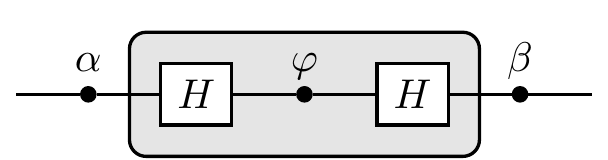
\includegraphics{quantum-info_files/figure-latex/unnamed-chunk-22-1} \end{center}

  Suppose you can control the input of the circuit and measure the output, but you do not know the phase shift \(\varphi\) introduced by the phase gate.
  You prepare input \(|0\rangle\) and register output \(|1\rangle\).
  What can you say about \(\varphi\)?

  Now you are promised that \(\varphi\) is either \(0\) or \(\pi\).
  You can run the circuit only once to find out which of the two phases was chosen.
  Can you do that?
\item
  Derive the identity
  \[
     (\vec{a}\cdot\vec{\sigma})(\vec{b}\cdot\vec{\sigma})
     = (\vec{a}\cdot\vec{b})\operatorname{id}+ i(\vec{a}\times \vec{b})\cdot \vec{\sigma}.
   \]
  (All you need here are the Pauli matrices' commutation and anti-commutation relations, but it is instructive to derive the identity using the component notation, and below we give a sketch of how such a derivation would go.)

  First, notice that the products of Pauli matrices can be written succinctly as
  \[
    \sigma_{i}\sigma_{j}
    = \delta _{ij}\operatorname{id}+ i\varepsilon_{ijk}\,\sigma _{k},
   \]
  where \(\delta_{ij}\) is the Kronecker delta and \(\varepsilon_{ijk}\) is the \textbf{Levi-Civita symbol}:
  \[
    \varepsilon_{ijk}
    = \begin{cases}
     +1 & {\text{if }}(i,j,k){\text{ is }}(1,2,3)\text{, }(2,3,1){\text{, or }}(3,1,2)
   \\-1 & {\text{if }}(i,j,k){\text{ is }}(3,2,1)\text{, }(1,3,2){\text{, or }}(2,1,3)
   \\\;\;\;0 & {\text{if }}i=j,{\text{ or }}j=k,{\text{ or }}k=i
   \end{cases}
   \]
  That is, \(\varepsilon _{ijk}\) is \(1\) if \((i, j, k)\) is an even permutation of \((1, 2, 3)\), it is \(-1\) if it is an odd permutation, and it is \(0\) if any index is repeated.
  The Levi-Civita symbol is anti-symmetric, meaning when any two indices are changed, its sign alternates.
  Then recall that the scalar (dot) product and vector (cross) product of two Euclidean vectors \(\vec{a}\) and \(\vec{b}\) can be written, in terms of the components, as
  \[
     \begin{aligned}
       \vec{a}\cdot\vec{b}
       &= \sum_{i=1}^3 a_i b_i
     \\(\vec{a}\times\vec{b})_i
       &= \sum_{j,k=1}^3 \varepsilon_{ijk}a_jb_k.
     \end{aligned}
   \]
  The rest is rather straightforward:
  \[
     (\vec{a}\cdot\vec{\sigma})(\vec{b}\cdot\vec{\sigma})
     = \sum_{ij}a_i b_j\sigma_i\sigma_j
     = \ldots.
   \]
\end{enumerate}

\hypertarget{chapter3}{%
\section{Logic and geometry with quantum gates}\label{chapter3}}

\begin{quote}
About understanding the square root of \(\texttt{NOT}\) via a physical implementation using symmetric beam-splitters.
More about the Bloch sphere, via the omnipresent Pauli matrices, which can be described in a more algebraic way.
\end{quote}

Before moving on, we first study two of the subjects from \protect\hyperlink{chapter2}{Chapter 2} in more depth: the square root of \(\texttt{NOT}\), and the Bloch sphere.

The goal for the latter is to be able to visualise sequences of unitary operations on a qubit as sequences of rotations, and to see the action of some quantum circuits without getting engaged in lengthy calculations.
The goal for the former is to study a way of implementing this gate using physical experiments, and then studying a related construction (the so-called \textbf{Mach--Zehnder interferometer}).

\hypertarget{physics-against-logic-via-beamsplitters}{%
\subsection{Physics against logic, via beamsplitters}\label{physics-against-logic-via-beamsplitters}}

A symmetric beam-splitter is a cube of glass which reflects half the light that impinges upon it, while allowing the remaining half to pass through unaffected.
For our purposes it can be viewed as a device which has two input and two output ports which we label as \(|0\rangle\) and \(|1\rangle\), as in Figure \ref{fig:beam-splitter}.

\begin{figure}[H]

{\centering 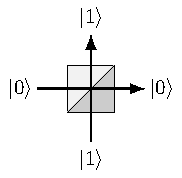
\includegraphics{quantum-info_files/figure-latex/beam-splitter-1} 

}

\caption{A beam-splitter.}\label{fig:beam-splitter}
\end{figure}

When we aim a single photon at such a beam-splitter using one of the input ports, we notice that the photon doesn't split in two: we can place photo-detectors wherever we like in the apparatus, fire in a photon, and verify that if any of the photo-detectors registers a hit, none of the others do.
In particular, if we place a photo-detector behind the beam-splitter in each of the two possible exit beams, the photon is detected with equal probability at either detector, no matter whether the photon was initially fired from input port \(|0\rangle\) or \(|1\rangle\).

It may seem obvious that, at the very least, the photon is \emph{either} in the transmitted beam \(|0\rangle\) \emph{or} in the reflected beam \(|1\rangle\) during any one run of this experiment.
Thus we may be tempted to think of the beam-splitter as a random binary switch which, with equal probability, transforms any binary input into one of the two possible outputs.
However, that is not necessarily the case.
Let us introduce a second beam-splitter and place two normal mirrors so that both paths intersect at the second beam-splitter, resulting in something resembling the Mach-Zehnder interferometer (see \ref{fig:two-beam-splitters}).

\begin{figure}[H]

{\centering 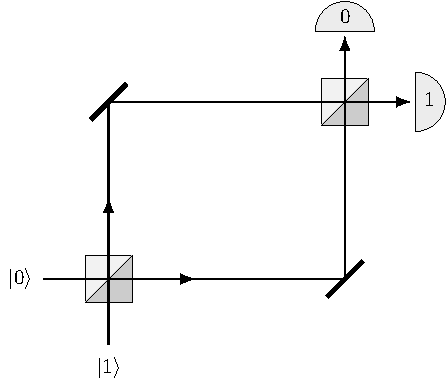
\includegraphics{quantum-info_files/figure-latex/two-beam-splitters-1} 

}

\caption{Two beam-splitters with mirrors, so that a photon travels through both.}\label{fig:two-beam-splitters}
\end{figure}

Now, the axiom of additivity in probability theory says that whenever something can happen in several alternative ways we add probabilities for each way considered separately.
We might argue that a photon fired into the input port \(|0\rangle\) can reach the detector \(0\) in two \emph{mutually exclusive} ways: either by two consecutive reflections or by two consecutive transmissions.
Each reflection happens with probability \(1/2\) and each transmission happens with probability \(1/2\) thus the total probability of reaching detector 0 is a sum of the probability of the two consecutive reflections (\(1/2\times 1/2 = 1/4\)) and the probability of the two consecutive transmissions (\(1/2\times 1/2 = 1/4\)) which gives probability \(1/2\).
This is summarised in \ref{fig:classical-guess-double-beam-splitter}, and makes perfect sense --- a random switch followed by a random switch should give nothing else but a random switch.
However, if we set up such an experiment, that is not what happens!

\begin{idea}

There is no reason why probability theory or any other a priori mathematical construct should make any meaningful statements about outcomes of physical experiments.

\end{idea}

\begin{figure}[H]

{\centering 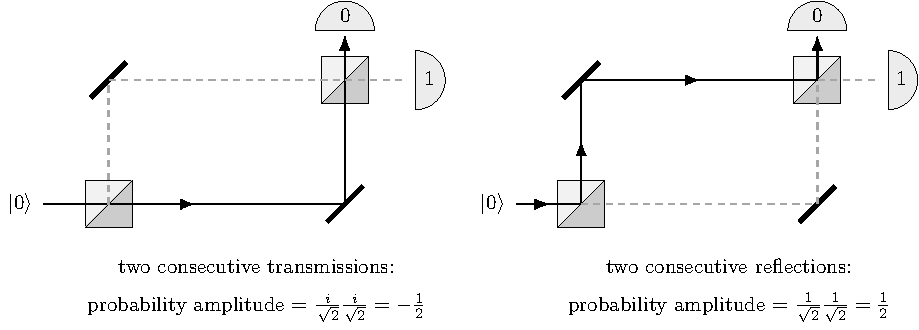
\includegraphics{quantum-info_files/figure-latex/classical-guess-double-beam-splitter-1} 

}

\caption{The two possible classical scenarios. Note that this is **not** what actually happens in the real physical world!}\label{fig:classical-guess-double-beam-splitter}
\end{figure}

In experimental reality, when the optical paths between the two beam-splitters are the same, the photon fired from input port \(|0\rangle\) \emph{always} strikes detector 1 and \emph{never} detector 0 (and the photon fired from input port \(|1\rangle\) \emph{always} strikes detector 0 and \emph{never} detector 1).
Thus a beam-splitter acts as the square root of \(\texttt{NOT}\) gate.

The action of the beam-splitter --- in fact, the action of any quantum device --- can be described by tabulating the amplitudes of transitions between its input and output ports.\footnote{Note that gate \(B\) is not the same square root of \(\texttt{NOT}\) as the one described in the first diagram in this section. There are infinitely many ways of implementing this ``impossible'' logical operation.}
\begin{equation}
  B = 
  \begin{bmatrix}
  B_{00} & B_{01}\\
  B_{10} & B_{11}
  \end{bmatrix}
  =
  \begin{bmatrix}
  \frac{1}{\sqrt 2} & \frac{i}{\sqrt 2}\\
  \frac{i}{\sqrt 2} & \frac{1}{\sqrt 2}
  \end{bmatrix}.
\label{eq:beam-splitter}
\end{equation}
The matrix element \(B_{lk}\), where \(k,l=0,1\), represents the amplitude of transition from input \(|k\rangle\) to output \(|l\rangle\) (watch the order of indices).
Each reflection (entries \(B_{01}\) and \(B_{10}\)) happens with amplitude \(i/\sqrt{2}\) and each transmission (entries \(B_{00}\) and \(B_{11}\)) happens with amplitude \(1/\sqrt{2}\).
Thus the total amplitude that a photon fired from input port \(|0\rangle\) will reach detector \(0\) is the sum of the amplitude of the two consecutive reflections (\(i/\sqrt{2}\times i/{\sqrt 2} = -1/2\)) and the amplitude of the two consecutive transmissions (\(1/{\sqrt 2}\times 1/{\sqrt 2} = 1/2\)) which gives the total amplitude \(0\).
The resulting probability is then zero.
Unlike probabilities, amplitudes can cancel out each other out.
We can now go on and calculate the amplitude that the photon will reach detector \(1\).
In this case we will get \(i\), which gives probability \(1\).
We can then switch to input \(|1\rangle\) and repeat our calculations.
All possible paths and associated amplitudes are shown in \ref{fig:paths-and-amplitudes-two-beam-splitters}.

\begin{figure}[H]

{\centering 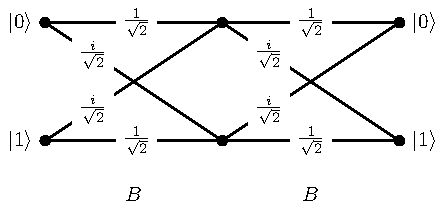
\includegraphics{quantum-info_files/figure-latex/paths-and-amplitudes-two-beam-splitters-1} 

}

\caption{All possible transitions and their amplitudes when we compose two beam-splitters $B$.}\label{fig:paths-and-amplitudes-two-beam-splitters}
\end{figure}

However, instead of going through all the paths in this diagram and linking specific inputs to specific outputs, we can simply multiply the transition matrices:
\[
  BB =
  \begin{bmatrix}
    \frac{1}{\sqrt 2} & \frac{i}{\sqrt 2}\\
    \frac{i}{\sqrt 2} & \frac{1}{\sqrt 2}
  \end{bmatrix}
  \begin{bmatrix}
    \frac{1}{\sqrt 2} & \frac{i}{\sqrt 2}\\
    \frac{i}{\sqrt 2} & \frac{1}{\sqrt 2}
  \end{bmatrix}
  =
  \begin{bmatrix}
  0 & i\\
  i & 0
  \end{bmatrix}
  = iX
\]
where \(X=\begin{bmatrix}0&1\\1&0\end{bmatrix}\) is the \(\texttt{NOT}\) operator.

Recalling \protect\hyperlink{the-square-root-of-not}{The square root of NOT}, we see that beam-splitters give a physical way of constructing the square root of \(\texttt{NOT}\).

\begin{idea}

\begin{longtable}[]{@{}cc@{}}
\toprule
\begin{minipage}[b]{(\columnwidth - 1\tabcolsep) * \real{0.40}}\centering
\(\texttt{NOT}\)\strut
\end{minipage} & \begin{minipage}[b]{(\columnwidth - 1\tabcolsep) * \real{0.60}}\centering
\(\sqrt{\texttt{NOT}}\)\strut
\end{minipage}\tabularnewline
\midrule
\endhead
\begin{minipage}[t]{(\columnwidth - 1\tabcolsep) * \real{0.40}}\centering
\(X = \begin{bmatrix}0&1\\1&0\end{bmatrix}\)\strut
\end{minipage} & \begin{minipage}[t]{(\columnwidth - 1\tabcolsep) * \real{0.60}}\centering
\(B = \frac{1}{\sqrt2}\begin{bmatrix}1&i\\i&1\end{bmatrix}\)\strut
\end{minipage}\tabularnewline
\begin{minipage}[t]{(\columnwidth - 1\tabcolsep) * \real{0.40}}\centering
bit flip\strut
\end{minipage} & \begin{minipage}[t]{(\columnwidth - 1\tabcolsep) * \real{0.60}}\centering
beam-splitter\strut
\end{minipage}\tabularnewline
\bottomrule
\end{longtable}

\end{idea}

\hypertarget{quantum-interference-revisited-still-about-beam-splitters}{%
\subsection{Quantum interference revisited (still about beam-splitters)}\label{quantum-interference-revisited-still-about-beam-splitters}}

One of the simplest quantum devices in which quantum interference can be controlled is a \textbf{Mach--Zehnder interferometer} --- see Figure \ref{fig:mach-zehnder}.



\begin{figure}[H]

{\centering 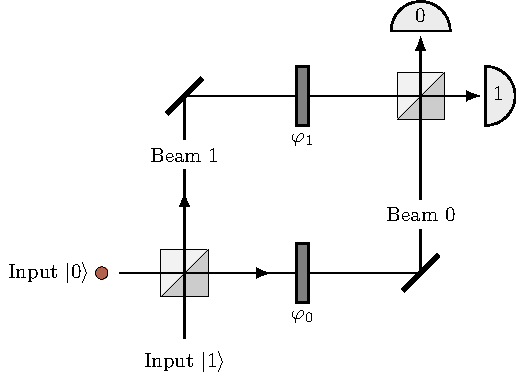
\includegraphics{quantum-info_files/figure-latex/mach-zehnder-1} 

}

\caption{The \href{https://en.wikipedia.org/wiki/Mach-Zehnder_interferometer}{Mach-Zehnder interferometer}, with the input photon represented by the coloured dot. This experimental set-up is named after the physicists Ludwig Mach and Ludwig Zehnder, who proposed it back in 1890s.}\label{fig:mach-zehnder}
\end{figure}

It consists of two beam-splitters (the square boxes, bottom left and top right) and two slivers of glass of different thickness which are inserted into each of the optical paths connecting the two beam-splitters.
The slivers are usually referred to as ``phase shifters'' and their thicknesses, \(\varphi_0\) and \(\varphi_1\), are measured in units of the photon's wavelength multiplied by \(2\pi\).
The two inputs ports of the interferometer are labelled as \(|0\rangle\) and \(|1\rangle\), and each of the two output ports, also labelled as \(0\) and \(1\), terminates in a photodetector.\footnote{The two diagonal objects in the top-left and bottom-right corners of \ref{fig:mach-zehnder} are simply mirrors to make the two possible paths meet at the second beam-splitter.}

A photon (the coloured dot in the figure) impinges on the first beam-splitter from one of the two input ports (here input 1) and begins its journey towards one of the two photodetectors.
Let\footnote{We will often use \(i\) as an index even though it is also used for the imaginary unit. Hopefully, no confusion will arise for it should be clear from the context which one is which.} \(U_{ij}\) denote the probability amplitude that the photon initially in input port \(j=0,1\) ends up in detector \(i=0,1\).
At each of the two beam-splitters the photon is transmitted with the probability amplitude \(\sqrt{T}\) and reflected with the probability amplitude \(i\sqrt{R}\), with \(R+T=1\), and the two phase shifters modify the amplitudes by phase factors \(e^{i\varphi_0}\) and \(e^{i\varphi_1}\), respectively.
In quantum theory we almost always start with the amplitudes, and once we have a full expression for the amplitude of a given outcome we square its absolute value to get the corresponding probability.
For example, let us calculate \(U_{00}\).

We notice that there are two alternative ways for the photon in the input port \(0\) to end up in the output port \(0\).
It can take the lower path, through the phase shifter \(\varphi_0\), or the upper path, through the phase shifter \(\varphi_1\).
The lower path implies two consecutive transmissions at the beam-splitters and the phase factor \(e^{i\varphi_0}\), whereas the upper path implies two consecutive reflections and the phase factor \(e^{i\varphi_1}\).
Once the photon ends in the output port \(0\) there is no way of knowing which path was taken, thus we add the amplitudes pertaining to each path.
The resulting amplitude is
\[
  U_{00}
  = \sqrt{T} e^{i\varphi_0} \sqrt{T}
  + i\sqrt{R} e^{i\varphi_1} i \sqrt{R},
\]
and the corresponding probability \(P_{00}=|U_{00}|^2\) reads
\[
  \begin{aligned}
    P_{00}
    & = \left\vert
          \sqrt{T}e^{i\varphi_0}\sqrt{T} + i\sqrt{R}e^{i\varphi_1}i\sqrt{R}
        \right\vert^2
      = \left\vert
          Te^{i\varphi_0} - Re^{i\varphi_1}
        \right\vert^2
  \\& = T^2 + R^2
        - 2TR\cos(\varphi_1-\varphi_0).
  \end{aligned}
\]

The ``classical'' part of this expression, \(T^2+R^2\), basically says that the photon undergoes either two consecutive transmissions with probability \(T^2\), or two consecutive reflections with probability \(R^2\).
The probability of being transmitted through any phase shifter is always \(1\), hence the phase shifters play no role in the classical description of this process.
But the classical description is not correct, as the experiments show, whence the interference term \(2TR\cos(\varphi_1-\varphi_0)\) in which the phase shifters play the essential role.
Depending on the \emph{relative} phase \(\varphi=\varphi_1-\varphi_0\) the probability that the detector \(0\) ``clicks'' can vary from \((T-R)^2\), for \(\varphi=0\), to \(1\), for \(\varphi=\pi\).

\begin{center}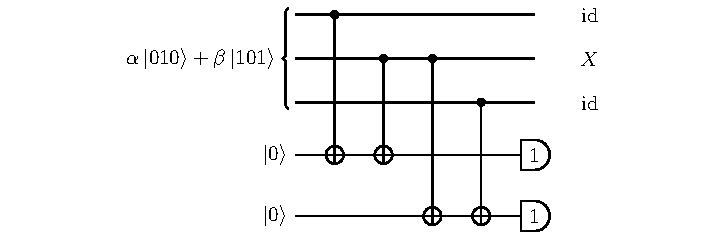
\includegraphics{quantum-info_files/figure-latex/unnamed-chunk-23-1} \end{center}

If we do not care about the experimental details, we can represent the action of the Mach--Zehnder interferometer in terms of a diagram: see \ref{fig:mach-zehnder-diagram}.

\begin{figure}[H]

{\centering 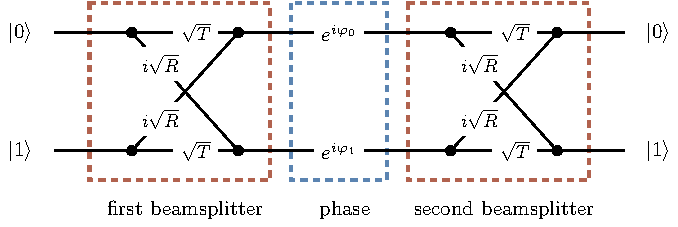
\includegraphics{quantum-info_files/figure-latex/mach-zehnder-diagram-1} 

}

\caption{The Mach-Zehnder interferometer represented as an abstract diagram.}\label{fig:mach-zehnder-diagram}
\end{figure}

Here we can follow, from left to right, the multiple different paths that a photon can take in between specific input and output ports.
The amplitude along any given path is just the product of the amplitudes pertaining to the path segments (Rule 1), while the overall amplitude is the sum of the amplitudes for the many different paths (Rule 2). You can, for example, see that the probability amplitude \(U_{10}\) is given by
\[
  U_{10}
  = \sqrt{T}e^{i\varphi_0}i\sqrt{R} + i\sqrt{R}e^{i\varphi_1}\sqrt{T}
\]
and the corresponding probability is
\[
  \begin{aligned}
    P_{10}
    & = \left\vert
        \sqrt{T}e^{i\varphi_0}i\sqrt{R} + i\sqrt{R}e^{i\varphi_1}\sqrt{T}
      \right\vert^2
  \\& = 2RT + 2RT\cos(\varphi_1-\varphi_0).
  \end{aligned}
\]
Again, the first term is of ``classical'' origin and represents probabilities corresponding to each path: one reflection followed by one transmission plus one transmission followed by one reflection, that is, \(RT+TR=2RT\).
The second term is the interference term.
Clearly, the photon entering port \(1\) will end up in one of the two detectors, hence,
\[
  P_{00} + P_{10}
  = R^2 + 2RT + T^2
  = (T+R)^2
  = 1.
\]
The action of the interferometer is thus fully described\footnote{In general, any isolated quantum device, including a quantum computer, can be described by a matrix of probability amplitudes \(U_{ij}\) that input \(j\) generates output \(i\). Watch the order of indices.} by the four probability amplitudes \(U_{ij}\) (\(i,j=0,1\)).
The most popular instance of a Mach--Zehnder interferometer involves only symmetric beam-splitters \((R=T=\frac12)\) and is fully described by the matrix
\[
  U =
  \begin{bmatrix}
    -\sin\varphi/2 & \cos\varphi/2
  \\\cos\varphi/2 & \sin\varphi/2
  \end{bmatrix}
\]
where \(\varphi=\varphi_1-\varphi_0\).
In fact, when you do all the calculations you obtain \(ie^{i\frac{\varphi_0+\varphi_1}{2}}U\) rather than \(U\), but the global phase factor \(ie^{i\frac{\varphi_0+\varphi_1}{2}}\) is common to all the amplitudes in the matrix and as such it does not contribute to the resulting probabilities.\footnote{Why is this? Hint: think about the eigenvalues of a matrix \(A\) and of the matrix \(\mu A\), where \(\mu\) is a complex number with \(|\mu|=1\).}

\hypertarget{the-pauli-matrices-algebraically}{%
\subsection{The Pauli matrices, algebraically}\label{the-pauli-matrices-algebraically}}

Matrices form a vector space: you can add them, and you can multiply them by a scalar.
One possible choice of a basis in the vector space of \((2\times 2)\) matrices is the set of matrices \(\{M_{00},M_{01},M_{10},M_{11}\}\), where the entries of \(M_{ij}\) are all \(0\) except for the \(ij\)-th entry, which is \(1\) (e.g.~\(M_{01}=\begin{bmatrix}0&1\\0&0\end{bmatrix}\)).
However, it turns out that there is a different basis which offers lots of insights into the structure of the general single-qubit unitary transformations, namely \(\{\operatorname{id},X,Y,Z\}\), i.e.~the identity matrix and the three Pauli matrices.

\begin{idea}

\begin{longtable}[]{@{}cccc@{}}
\toprule
\begin{minipage}[b]{(\columnwidth - 3\tabcolsep) * \real{0.25}}\centering
\(\operatorname{id}\)\strut
\end{minipage} & \begin{minipage}[b]{(\columnwidth - 3\tabcolsep) * \real{0.25}}\centering
\(X=\sigma_x\)\strut
\end{minipage} & \begin{minipage}[b]{(\columnwidth - 3\tabcolsep) * \real{0.25}}\centering
\(Y=\sigma_y\)\strut
\end{minipage} & \begin{minipage}[b]{(\columnwidth - 3\tabcolsep) * \real{0.25}}\centering
\(Z=\sigma_z\)\strut
\end{minipage}\tabularnewline
\midrule
\endhead
\begin{minipage}[t]{(\columnwidth - 3\tabcolsep) * \real{0.25}}\centering
\(\begin{bmatrix}1&0\\0&1\end{bmatrix}\)\strut
\end{minipage} & \begin{minipage}[t]{(\columnwidth - 3\tabcolsep) * \real{0.25}}\centering
\(\begin{bmatrix}0&1\\1&0\end{bmatrix}\)\strut
\end{minipage} & \begin{minipage}[t]{(\columnwidth - 3\tabcolsep) * \real{0.25}}\centering
\(\begin{bmatrix}0&-i\\i&0\end{bmatrix}\)\strut
\end{minipage} & \begin{minipage}[t]{(\columnwidth - 3\tabcolsep) * \real{0.25}}\centering
\(\begin{bmatrix}1&0\\1&-1\end{bmatrix}\)\strut
\end{minipage}\tabularnewline
\bottomrule
\end{longtable}

\end{idea}

Recalling \protect\hyperlink{pauli-operators}{Pauli operators}, we know that the Pauli operators (as well as the identity operator) are unitary and Hermitian, square to the identity, and anti-commute.

Any \((2\times 2)\) complex matrix \(A\) has a unique expansion in the form
\begin{equation}
  \begin{aligned}
    A &=
    \begin{bmatrix}
      a_0 + a_z & a_x - i a_y
    \\a_x +i a_y &  a_0 - a_z
    \end{bmatrix}
  \\&= a_0\operatorname{id}+ a_x \sigma_x + a_y \sigma_y + a_z \sigma_z
  \\&= a_0\operatorname{id}+ \vec{a}\cdot\vec{\sigma}.
  \end{aligned}
\label{eq:pauli}
\end{equation}
for some complex numbers \(a_0\), \(a_x\), \(a_y\), and \(a_z\).
Here, \(\vec{a}\) is a vector with three complex components \((a_x, a_y, a_z)\), and \(\vec{\sigma}\) represents the ``vector'' of Pauli matrices \((\sigma_x,\sigma_y,\sigma_z)\).
The algebraic properties of the Pauli matrices can be neatly compacted (see the exercises) into a single expression:

The \textbf{multiplication rule}:
\[
  (\vec{a}\cdot\vec{\sigma})\,(\vec{b}\cdot\vec{\sigma})
  = (\vec{a}\cdot\vec{b})\,\operatorname{id}+ i(\vec{a}\times \vec{b})\cdot\vec{\sigma}.
\]

We also introduce the inner product of two matrices:

The \textbf{Hilbert--Schmidt product}:
\[
  (A|B) = \frac12 \operatorname{tr}A^\dagger B.
\]

Recall that the trace of a square matrix \(A\), denoted by \(\operatorname{tr}A\), is defined to be the sum of the elements on the main diagonal of \(A\), and defines a linear mapping: for any scalars \(\alpha\) and \(\beta\),
\[
  \operatorname{tr}(\alpha A+\beta B) = \alpha\operatorname{tr}A +\beta\operatorname{tr}B.
\]
Moreover, the trace is invariant under \emph{cyclic} permutations: e.g.
\[
  \operatorname{tr}(ABC) = \operatorname{tr}(BCA) = \operatorname{tr}(CAB).
\]
Note, however, that this does \emph{not} imply that e.g.~\(\operatorname{tr}(ABC)=\operatorname{tr}(ACB)\).

\hypertarget{exercises-1}{%
\subsubsection{Exercises}\label{exercises-1}}

\begin{enumerate}
\def\labelenumi{\arabic{enumi}.}
\item
  Show that \(\{\operatorname{id},\sigma_x,\sigma_y,\sigma_z\}\) is an orthonormal basis with respect to the Hilbert-Schmidt product in the space of complex \((2\times 2)\) matrices.
\item
  Show that the coefficients \(a_k\) (for \(k=x,y,z\)) in Equation \eqref{eq:pauli} are given by the inner product \(a_k = (\sigma_k|A) = \frac12\operatorname{tr}\sigma_k A\).
\item
  Show that \(\frac12\operatorname{tr}(\vec{a}\cdot\vec{\sigma})(\vec{b}\cdot\vec{\sigma}) = \vec{a}\cdot\vec{b}\).
\item
  Show that any \(\vec{n}\cdot\vec{\sigma}\) has eigenvalues are \(\pm|\vec{n}|\).
\item
  Show that, if \(\vec{n}\cdot\vec{m}=0\), then the operators \(\vec{n}\cdot\vec{\sigma}\) and \(\vec{m}\cdot\vec{\sigma}\) anticommute.
\item
  In these notes, we usually deal with matrices that are Hermitian (\(A=A^\dagger\)) or unitary (\(AA^\dagger=\operatorname{id}\)).
  It is easy to see that, if \(A\) is Hermitian, then \(a_0\) and the three components of \(\vec{a}\) are all real.
  The \((2\times 2)\) unitaries are usually parametrised as
  \[
     U = e^{i\gamma}\Big(u_0\operatorname{id}+ i(u_x\sigma_x + u_y\sigma_y + u_z\sigma_z)\Big)
   \]
  where \(e^{i\gamma}\) is an overall multiplicative phase factor, with \(\gamma\) real, and \(u_0\) and the three components \(u_x\), \(u_y\), \(u_z\) are all real numbers.

  Show that the unitarity condition implies that
  \[
     u_0^2 + u_x^2 + u_y^2 + u_z^2 = 1,
   \]
  and show that the determinant of \(U\) is \(e^{i2\gamma}\) using this parametrisation.
\end{enumerate}

\hypertarget{the-pauli-matrices-geometrically}{%
\subsection{The Pauli matrices, geometrically}\label{the-pauli-matrices-geometrically}}

Geometrically speaking, the group of unitaries \(\mathrm{U}(2)\) is a three-dimensional sphere \(S^3\) in \(\mathbb{R}^4\).
We often fix the determinant to be \(+1\) and express \((2\times 2)\) unitaries as
\[
  U = u_0\operatorname{id}+ i(u_x\sigma_x + u_y\sigma_y + u_z\sigma_z).
\]
Such matrices form a popular subgroup of \(\mathrm{U}(2)\); it is called the \textbf{special} (meaning the determinant is equal to \(1\)) unitary group, and denoted by \(\mathrm{SU}(2)\).
In quantum theory, any two unitary matrices that differ by some global multiplicative phase factor represent the same physical operation, so we are ``allowed to'' fix the determinant to be \(+1\), and thus restrict ourselves to considering matrices in \(\mathrm{SU}(2)\).
This is a sensible approach, practised by many theoretical physicists, but again, for some historical reasons, the convention in quantum information science does not follow this approach.
For example, phase gates are usually written as
\[
  P_\alpha = \begin{bmatrix}1&0\\0&e^{i\alpha}\end{bmatrix}
\]
rather than
\[
  P_\alpha = \begin{bmatrix}e^{-i\frac{\alpha}{2}}&0\\0&e^{\,i\frac{\alpha}{2}}\end{bmatrix}
\]
Still, sometimes the \(T\) gate
\[
  T
  = \begin{bmatrix}1&0\\0&e^{i\pi/4}\end{bmatrix}
  = \begin{bmatrix}e^{-i\pi/8}&0\\0&e^{i\pi/8}\end{bmatrix}
\]
is called the \(\pi/8\) gate, because of its \(\mathrm{SU}(2)\) form.

Let us write any \((2\times 2)\) unitary, up to an overall phase factor, as
\[
  U
  = u_0\operatorname{id}+ i(u_x \sigma_x + u_y \sigma_y + u_z \sigma_z)
  = u_0\operatorname{id}+ i{\vec{u}}\cdot{\vec{\sigma}}
\]
where \(u_0^2+|\vec{u}|^2=1\).
This additional unitarity restriction allows us to parametrise \(u_0\) and \(\vec{u}\) in terms of a real unit vector \(\vec{n}\), parallel to \(\vec{u}\), and a real angle \(\theta\) so that\footnote{As you can see, we often make progress and gain insights simply by choosing a convenient parametrisation.}
\[
  U
  = (\cos\theta)\operatorname{id}+ (i\sin\theta){\vec{n}}\cdot{\vec{\sigma}}.
\]
An alternative way of writing this expression is
\[
  U
  = e^{i\theta {\vec{n}}\cdot{\vec{\sigma}}},
\]
as follows from the power-series expansion of the exponential.
Indeed, any unitary matrix can always be written in the exponential form as
\[
  \begin{aligned}
    e^{iA}
    &\equiv \operatorname{id}+ iA + \frac{(i A)^2}{1\cdot 2} + \frac{(i A)^3}{1\cdot 2\cdot 3} \ldots
  \\&= \sum_{n=0}^\infty \frac{(i A)^n}{n!}
  \end{aligned}
\]
where \(A\) is a Hermitian matrix.

Writing unitary matrices in the form \(e^{iA}\) is analogous to writing complex numbers of unit modulus as \(e^{i\alpha}\) (the so-called polar form).

\hypertarget{exercises-2}{%
\subsubsection{Exercises}\label{exercises-2}}

\begin{enumerate}
\def\labelenumi{\arabic{enumi}.}
\tightlist
\item
  Show that, if \(A^2=\operatorname{id}\), then we can turn the power series expansion into a simple expression: for any real \(\alpha\),
  \[
     e^{i\alpha A}
     = (\cos\alpha)\operatorname{id}+ (i\sin\alpha)A.
   \]
\item
  Using the previous exercise, or otherwise, show that any \((2\times 2)\) unitary matrix \(U\) can be written, up to an overall multiplicative phase factor, as
  \[
     U
     = e^{i \theta \vec{n}\cdot\vec{\sigma}}
     = (\cos\theta)\operatorname{id}+ (i\sin\theta)\vec{n}\cdot\vec{\sigma}.
   \]
  (The argument here is the same as the argument that \(e^{i\theta}=\cos\theta +i\sin\theta\)).
\end{enumerate}

\hypertarget{unitaries-as-rotations}{%
\subsection{Unitaries as rotations}\label{unitaries-as-rotations}}

Here comes a remarkable connection between two-dimensional unitary matrices and ordinary three-dimensional rotations.

The unitary \(U = e^{i\theta \vec{n}\cdot\vec{\sigma}}\) represents a clockwise rotation through the angle \(2\theta\) about the axis defined by \(\vec{n}\).

(N.B. \(2\theta\), not \(\theta\)).

For example,
\[
  \begin{aligned}
    e^{i\theta\sigma_x}
    &=
    \begin{bmatrix}
      \cos\theta & i\sin\theta
    \\i\sin\theta & \cos\theta
    \end{bmatrix}
  \\e^{i\theta\sigma_y}
    &=
    \begin{bmatrix}
      \cos\theta & \sin\theta
    \\-\sin\theta & \cos\theta
    \end{bmatrix}
  \\e^{i\theta\sigma_z}
    &= \begin{bmatrix}e^{i\theta}&0\\0&e^{-i\theta}\end{bmatrix}
  \end{aligned}
\]
represent rotations by \(2\theta\) about the \(x\)-, \(y\)- and \(z\)-axis, respectively.



\begin{figure}[H]

{\centering 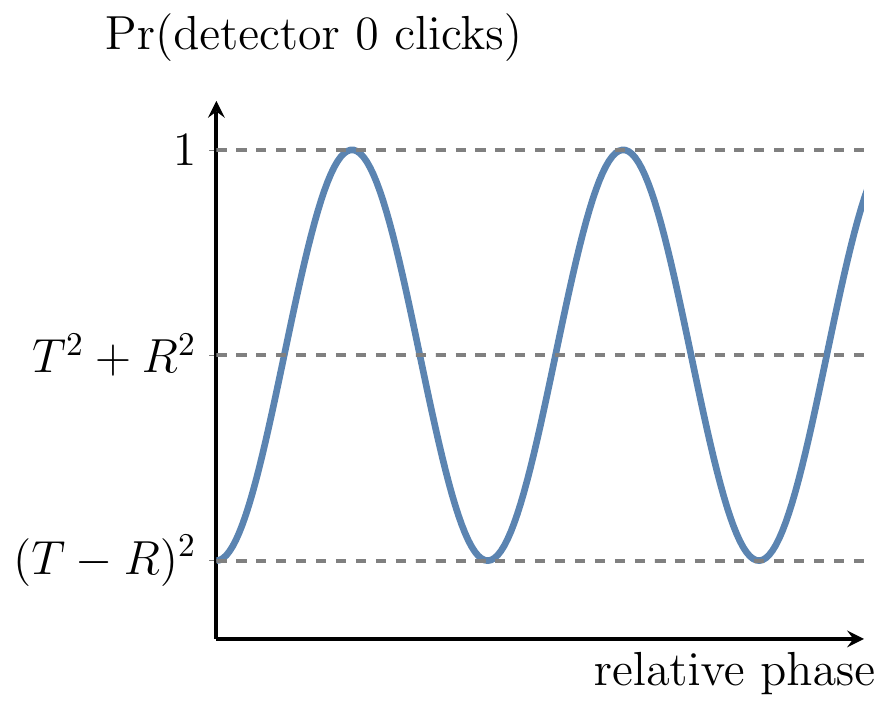
\includegraphics{quantum-info_files/figure-latex/unnamed-chunk-24-1} 

}

\caption{\(e^{i\theta\vec{n}\cdot\vec{\sigma}}\) rotates the vector \(\vec{s}\) about \(\vec{n}\) by angle \(2\theta\), sending it to a point on the blue circle, whose centre is passed through by \(\vec{n}\).}\label{fig:unnamed-chunk-24}
\end{figure}

The Hadamard gate
\[
  \begin{aligned}
    H
    &= \frac{1}{\sqrt 2}
    \begin{bmatrix}
      1& 1
    \\1 & -1
    \end{bmatrix}
  \\&= \frac{1}{\sqrt 2}(\sigma_x + \sigma_z)
  \\&= (-i)e^{i \frac{\pi}{2} \frac{1}{\sqrt 2}(\sigma_x+\sigma_z)}
  \end{aligned}
\]
(which, up to the overall multiplicative phase factor of \(-i\), is equal to \(e^{i \frac{\pi}{2} \frac{1}{\sqrt 2}(\sigma_x+\sigma_z)}\)) represents rotation about the diagonal \((x+z)\)-axis through the angle \(\pi\).

In somewhat abstract terms, we make the connection between unitaries and rotations by looking how the unitary group \(\mathrm{U}(2)\) acts on the three-dimensional Euclidian space of \((2\times 2)\) Hermitian matrices \emph{with zero trace}.
All such matrices \(S\) can be written as \(S=\vec{s}\cdot\vec{\sigma}\) for some real \(\vec{s}\), i.e.~each matrix is represented by a Euclidean vector \(\vec{s}\) in \(\mathbb{R}^3\).
Now, \(U\in \mathrm{U}(2)\) acts on the Euclidean space of such matrices by \(S\mapsto S' = USU^\dagger\), i.e.
\begin{equation}
  \vec{s}\cdot\vec{\sigma}
  \mapsto
  \vec{s'}\cdot\vec{\sigma}
  = U(\vec{s}\cdot\vec{\sigma})U^\dagger
\label{eq:u2so3map}
\end{equation}
This is a linear map \(\mathbb{R}^3\to\mathbb{R}^3\), and is thus given by some \((3\times 3)\) real-valued matrix \(R\).
We note that this map is an isometry (a distance preserving operation), since it preserves the scalar product in the Euclidean space: for any two vectors \(\vec{s}\) and \(\vec{v}\),
\[
  \begin{aligned}
    \vec{s'}\cdot\vec{v'}
    &= \frac12\operatorname{tr}[S'V']
  \\&= \frac12\operatorname{tr}[(USU^\dagger)(UVU^\dagger)]
  \\&= \frac12\operatorname{tr}[SV]
  \\&= \vec{s}\cdot\vec{v}
  \end{aligned}
\]
(where \(S=\vec{s}\cdot\vec{\sigma}\) and \(V=\vec{v}\cdot\vec{\sigma}\)), using the cyclic property of the trace.
This means that matrix \(R\) is \emph{orthogonal}.\footnote{Orthogonal transformations preserve the length of vectors as well as the angles between them.}
Furthermore, we can show\footnote{One can also infer that \(\det R=1\) from the fact that any matrix in \(\mathrm{U}(2)\) can be smoothly connected to the identity.} that \(\det R=1\).
The only isometries in three dimensional Euclidian space, which are described by orthogonal matrices \(R\) with \(\det R=1\), are rotations.
Thus, in the mathematical lingo, we have established a homomorphism\footnote{Recall that a homomorphism is a structure-preserving map between two algebraic structures of the same type, in our case two groups. An isomorphism between algebraic structures of the same type is one-to-one homomorphism.} between \(\mathrm{U}(2)\) and \(\mathrm{SO}(3)\), where \(\mathrm{SO}(3)\) stands for the special orthogonal group in three dimensions (the group of all rotations about the origin of three-dimensional Euclidean space \(\mathbb{R}^3\) under the operation of composition).
It is quite clear from Equation \eqref{eq:u2so3map} that unitary matrices differing only by a global multiplicative phase factor (e.g.~\(U\) and \(e^{i\gamma}U\)) represent the same rotation.

Physicists, however, usually prefer a more direct demonstration, which goes roughly like this.
Consider the map \(\vec{s} \mapsto \vec{s'}\) induced by \(U=e^{i \alpha \vec{n}\cdot\vec{\sigma}}\).
For small values of \(\alpha\), we can write
\[
  \begin{aligned}
    \vec{s'}\cdot\vec{\sigma}
    &= U(\vec{s}\cdot\vec{\sigma}) U^\dagger
  \\&= \Big(
      \operatorname{id}+i\alpha (\vec{n}\cdot\vec{\sigma})+\ldots
    \Big)
    (\vec{s}\cdot\vec{\sigma}) 
    \Big(
      \operatorname{id}- i\alpha(\vec{n}\cdot\vec{\sigma})+\ldots
    \Big).
  \end{aligned}
\]
To the first order in \(\alpha\), this gives
\[
  \vec{s'} \cdot\vec{\sigma}
  = \Big(
    \vec{s} + 2\alpha (\vec{n}\times\vec{s})
  \Big)
  \cdot \vec{\sigma}
\]
that is,
\[
  \vec{s'} =
  \vec{s} + 2\alpha(\vec{n}\times\vec{s})
\]
which we recognise as a good old textbook formula for an infinitesimal clockwise rotation of \(\vec{s}\) about the axis \(\vec{n}\) through the angle \(2\alpha\).

\hypertarget{exercises-3}{%
\subsubsection{Exercises}\label{exercises-3}}

\emph{In some of these exercises, we continue to study the \((3\times 3)\) real-valued matrix \(R\) described above.}

\begin{enumerate}
\def\labelenumi{\arabic{enumi}.}
\tightlist
\item
  Show that \(\operatorname{tr}\sigma_x\sigma_y\sigma_z = 2i\).
\item
  Consider
  \[
     U(\vec e_k\cdot\sigma_k)U^\dagger=U\sigma_kU^\dagger={\vec f_k}\cdot\vec\sigma.
   \]
  So \(U\) maps the unit vectors \(\vec e_x\), \(\vec e_y\), and \(\vec z_z\), (along the \(x\)-, \(y\)-, and \(z\)-axis, respectively), to new unit vectors \(\vec f_x\), \(\vec f_y\), and \(\vec f_z\).
  We already know that, in Euclidean space, this transformation is described by a \((3\times 3)\) orthogonal matrix \(R\).
  How are the three vectors \(\vec f_x\), \(\vec f_y\), and \(\vec f_z\) related to the entries in matrix \(R\)?
\item
  Show that
  \[
     \begin{aligned}
       \operatorname{tr}\sigma_x\sigma_y\sigma_z
       &= \operatorname{tr}({\vec f_x}\cdot\vec\sigma)( {\vec f_y}\cdot\vec\sigma)({\vec f_z}\cdot\vec\sigma)
     \\&= 2i\det R
     \end{aligned}
   \]
  (which implies that \(\det R=1\)).
\item
  Make use of the orthonormality of the Pauli basis and Equation \eqref{eq:u2so3map} to show that the elements of the matrix \(R\) can be expressed in terms of those of the matrix \(U\), in the form
  \[
     R_{ij}=\frac12\operatorname{tr}\left(\sigma_i U\sigma_j U^\dagger\right).
   \]
  Here, \(i\) and \(j\) take values in \(\{1,2,3\}\), and \(\sigma_1\equiv\sigma_x\), \(\sigma_2\equiv\sigma_y\), \(\sigma_3\equiv\sigma_z\).
\item
  Show that the phase gate \(P_\varphi =\begin{bmatrix}1&0\\0&e^{i\varphi}\end{bmatrix}\) represents an anticlockwise rotation about the \(z\)-axis through the angle \(\varphi\).
  Note that it might be helpful to start with the \(\mathrm{SU}(2)\) version of the phase gate:
  \[
     \begin{aligned}
       P_\varphi
       &= e^{-i\frac{\varphi}{2}\sigma_z}
     \\&= \begin{bmatrix}
         e^{-i \frac{\varphi}{2}}& 0
       \\0 & e^{i \frac{\varphi}{2}}
       \end{bmatrix}
       \quad\longrightarrow\quad
       R
     \\&= \begin{bmatrix}
         \cos \varphi & -\sin \varphi & 0
       \\\sin \varphi & \cos \varphi & 0
       \\0 & 0 & 1
       \end{bmatrix}
     \end{aligned}
   \]
\item
  Express the Hadamard gate \(H\) in terms of \(\vec{n}\cdot\vec{\sigma}\), and demonstrate that
  \[
     \begin{aligned}
       HZH&=X
     \\HXH&=Z
     \\HYH&=-Y.
     \end{aligned}
   \]
\item
  Show that the Hadamard gate \(H\) turns rotations about the \(x\)-axis into rotations about the \(z\)-axis, and vice versa.
  That is,
  \[
     \begin{aligned}
       H \left(
         e^{-i\frac{\varphi}{2}Z}
       \right) H
       &= e^{-i\frac{\varphi}{2}X}
       \qquad \mbox{and} \qquad
       H \left(
         e^{-i\frac{\varphi}{2}X}
       \right) H
     \\&= e^{-i\frac{\varphi}{2}Z}.
     \end{aligned}
   \]
\end{enumerate}

\hypertarget{universality-again}{%
\subsection{Universality, again}\label{universality-again}}

Although this may all seem tediously abstract, it is surprisingly useful.
Take another look at the single qubit interference circuit

\begin{center}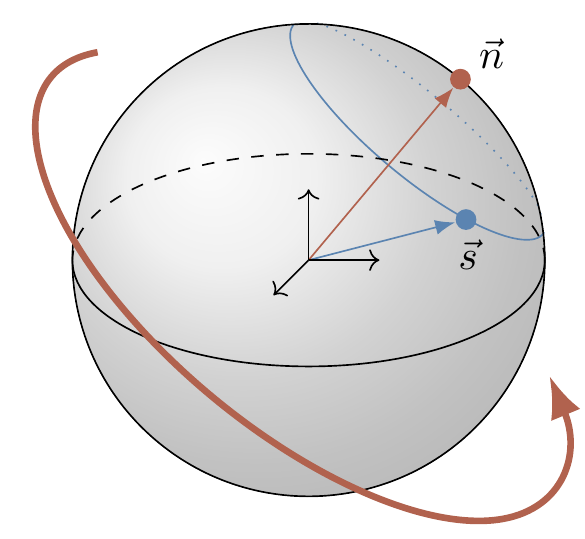
\includegraphics{quantum-info_files/figure-latex/unnamed-chunk-25-1} \end{center}

and the corresponding sequence of unitary operations
\[
  \begin{aligned}
    H \left(
      e^{-i\frac{\varphi}{2}Z}
    \right) H
    &= e^{-i\frac{\varphi}{2}X}
  \\&= \begin{bmatrix}
      \cos\varphi/2 & -i\sin\varphi/2
    \\-i\sin\varphi/2 & \cos\varphi/2
    \end{bmatrix}
  \end{aligned}
\]

The single qubit interference circuit has a simple geometrical meaning: it shows how a rotation about the \(z\)-axis, induced by the phase gate \(P_\varphi\), is turned, by the two Hadamard gates, into a rotation about the \(x\)-axis.

Now, take a look at this circuit:

\begin{center}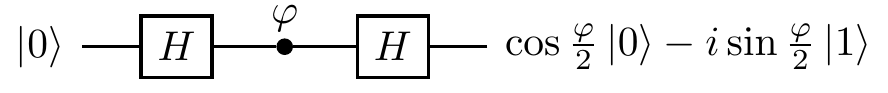
\includegraphics{quantum-info_files/figure-latex/unnamed-chunk-26-1} \end{center}

What does it represent?
The central part is a rotation by \(\varphi\) about the \(x\)-axis, but is it is sandwiched between two rotations about the \(z\)-axis.
Now I have to appeal to your knowledge of classical mechanics.
You may recall that any rotation in the Euclidean space can be performed as a sequence of three rotations: one about \(z\)-axis, one about \(x\)-axis, and one more about the \(z\)-axis.
In this context, this implies that any unitary \(U\), up to a global phase factor, can be written as
\[
  \begin{aligned}
    U(\alpha, \beta, \varphi)
    &= e^{-i\frac{\beta}{2}Z} e^{-i\frac{\varphi}{2}X} e^{-i\frac{\alpha}{2}Z}
  \\&= \begin{bmatrix}
      e^{-i\left(\frac{\alpha+\beta}{2}\right)}\cos\frac{\varphi}{2}
      & ie^{i\left(\frac{\alpha-\beta}{2}\right)}\sin\frac\varphi{2}
    \\ie^{-i\left(\frac{\alpha-\beta}{2}\right)}\sin\frac\varphi{2}
      & e^{i\left(\frac{\alpha+\beta}{2}\right)}\cos\frac\varphi{2}
    \end{bmatrix}.
  \end{aligned}
\]

Thus once you are given a couple of Hadamard gates and an infinite supply of phase gates, so that you can choose the three phases you need, you can construct an arbitrary unitary operation on a single qubit. Needless to say, the two axes in question, \(z\) and \(x\), do not have any special status, geometrically speaking --- if we have rotations about any two orthogonal\footnote{In fact, even this condition isn't necessary! See Figure \ref{fig:two-families-of-circles}} axes then we can create any one-qubit unitary that we want.



\begin{figure}[H]

{\centering 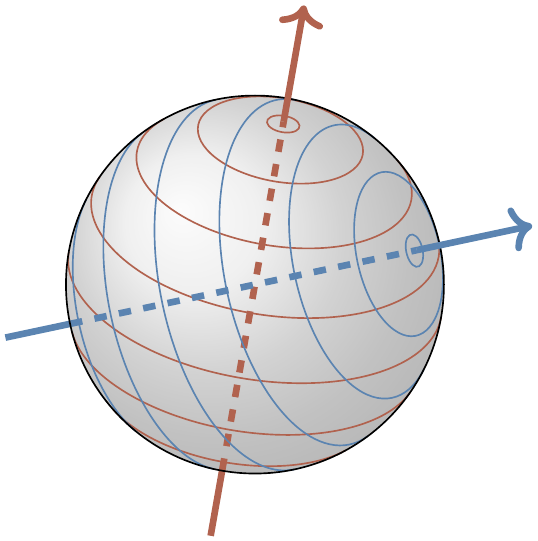
\includegraphics{quantum-info_files/figure-latex/two-families-of-circles-1} 

}

\caption{If we can move along the two families of circles, then from any point on the sphere we can reach any other point. The two axes do not even have to be orthogonal: any two different axes will do. Can you see why?}\label{fig:two-families-of-circles}
\end{figure}

Consider the following circuit:

\begin{center}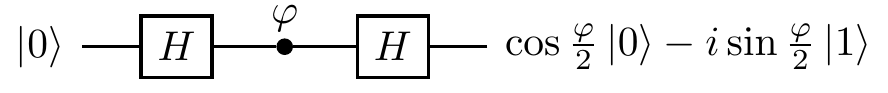
\includegraphics{quantum-info_files/figure-latex/unnamed-chunk-27-1} \end{center}

where both \(A\) and \(B\) are unitary operations.
We claim that \emph{any} unitary \(U\) can be represented in this form.

Again, we can prove this geometrically.
The circuit represents two rotations by \(180^\circ\) about two axes obtained by rotating the \(z\)-axis with unitaries \(A\) and \(B\), respectively.
Any rotation in the three-dimensional space is the composition of two rotations by \(180^\circ\), as shown in Figure \ref{fig:two-rotations-by-180}.
The resulting axis of rotation is perpendicular to the two axes about which rotations by \(180^\circ\) are performed, and the angle of the composed rotation is twice the angle between the two axes.



\begin{figure}[H]

{\centering 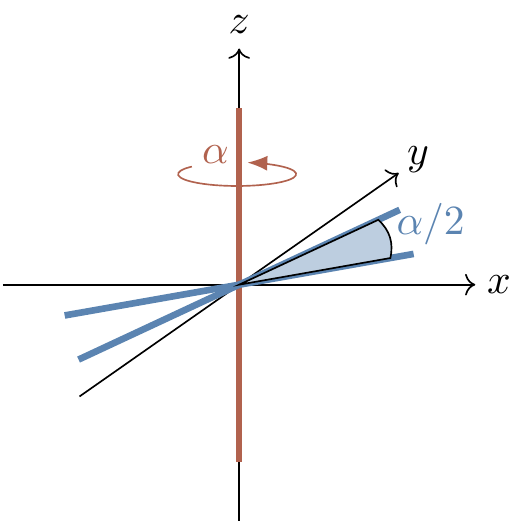
\includegraphics{quantum-info_files/figure-latex/two-rotations-by-180-1} 

}

\caption{Rotating by \(\alpha\) around the \(z\)-axis is the same as the composition of two rotations by \(180^\circ\) around axes which both lie in the \(xy\)-plane, with angle \(\alpha/2\) between them.}\label{fig:two-rotations-by-180}
\end{figure}

\hypertarget{exercises-4}{%
\subsubsection{Exercises}\label{exercises-4}}

\begin{enumerate}
\def\labelenumi{\arabic{enumi}.}
\tightlist
\item
  In the Singapore Botanic Gardens, there is a sculpture by Ueli Fausch called ``Swiss Granite Fountain''.
  It is a spherical granite ball which measures 80cm in diameter and weighs 700kg, and is kept afloat by strong water pressure directed through the basal block.
  It is easy to set the ball in motion, and it keeps rotating in whatever way you start for a long time.
  Suppose you are given access to this ball only near the top, so that you can push it to make it rotate around any horizontal axis, but you don't have enough of a grip to make it turn around the vertical axis.
  Can you make it rotate around the vertical axis anyway?
\end{enumerate}

\hypertarget{quantum-dynamics}{%
\subsection{Some quantum dynamics}\label{quantum-dynamics}}

The time evolution of a quantum state is a unitary process which is generated by a Hermitian operator called the \textbf{Hamiltonian}, which we also\footnote{Hopefully it will always be clear from the context which \(H\) refers to Hamiltonian and which \(H\) to Hadamard. Don't confuse the two!} denote by \(H\).
The Hamiltonian contains a complete specification of all interactions within the system under consideration.
In an isolated system, the state vector \(|\psi(t)\rangle\) changes smoothly in time according to the \textbf{Schrödinger equation}:
\[
  \frac{\mathrm{d}}{\mathrm{d}t} |\psi(t)\rangle
  =-\frac{i}{\hbar} H |\psi(t)\rangle.
\]
For time independent Hamiltonians\footnote{That is, where \(|\psi(t)\rangle=|\psi\rangle\) has no \(t\)-dependence.}, the formal solution of this reads\footnote{Here \(\hbar\) denotes \textbf{Planck's constant}, which has the value \mbox{$\hbar = 1.05\times 10^{-34}\,\mbox{\rm Js}$}. However, theorists always choose to work with a system of units where \(\hbar = 1\).}
\[
  \begin{gathered}
    |\psi(t)\rangle
    = U(t)|\psi(0)\rangle
  \\\quad\mbox{where}\quad
    U(t)
    = e^{-\frac{i}{\hbar}Ht}.
  \end{gathered}
\]

Now, to relate this to the earlier parts of this chapter, we note that the Hamiltonian of a qubit can always be written in the form \(H = E_0\operatorname{id}+\omega(\vec{n}\cdot\vec{\sigma})\), hence
\[
  \begin{aligned}
    U(t)
    &= e^{-i\omega t \vec n\cdot\vec\sigma}
  \\&= (\cos\omega t)\operatorname{id}- (i\sin\omega t)\vec{n}\cdot\vec{\sigma}
  \end{aligned}
\]
which is a rotation with angular frequency \(\omega\) about the axis defined by the unit vector \(\vec n\).

\textbf{!!!TODO!!! the \(4\pi\) world of qubits}

\hypertarget{exercises-5}{%
\subsubsection{Exercises}\label{exercises-5}}

\begin{enumerate}
\def\labelenumi{\arabic{enumi}.}
\tightlist
\item
  A qubit (spin one-half particle) initially in state \(|0\rangle\) (spin up) is placed in a uniform magnetic field.
  The interaction between the field and the qubit is described by the Hamiltonian
  \[
     H
     = \omega
     \begin{bmatrix}
       0 & - i
     \\i & 0
     \end{bmatrix}
   \]
  where \(\omega\) is proportional to the strength of the field.\footnote{In Earth's magnetic field, which is about \(0.5\) gauss, the value of \(\omega\) is of the order of \(10^6\) cycles per second.}
  What is the state of the qubit after time \(t=\pi/4\omega\)?
\end{enumerate}

\hypertarget{chapter4}{%
\section{Measurements}\label{chapter4}}

\begin{quote}
About the Hilbert-space formalism of quantum theory, and the role of \textbf{measurements} in quantum information theory, as well as introducing the quantum dramas of Alice and Bob.
\end{quote}

Eventually, we have to talk about quantum measurements, since, at some point, someone has to look at a measuring device and register the outcome of whatever quantum circuits we've been designing.
It turns out that this is a bit more tricky than one might think.
Quantum measurement is not a passive acquisition of information: if you measure, you disturb.
Even though it is a physical process, like any other quantum evolution, it is traditionally described by a different set of mathematical tools.

\hypertarget{hilbert-spaces-briefly}{%
\subsection{Hilbert spaces, briefly}\label{hilbert-spaces-briefly}}

A formal mathematical setting for a quantum system is that of a \textbf{Hilbert space} \(\mathcal{H}\), i.e.~a vector space with an inner product.
The result of any preparation of a system is represented by some unit vector \(|\psi\rangle\in \mathcal{H}\), and any test is represented by some other unit vector \(|e\rangle\in \mathcal{H}\).\footnote{The term ``Hilbert space'' used to be reserved for an infinite-dimensional inner product space that is \textbf{complete}, i.e.~such that every Cauchy sequence in the space converges to an element in the space. Nowadays, as in these notes, the term includes finite-dimensional spaces, which automatically satisfy the condition of completeness.}
The inner product of these two vectors, \(\langle e|\psi\rangle\), gives the probability amplitude that an object prepared in state \(|\psi\rangle\) will pass a test for being in state \(|e\rangle\).
Probabilities are obtained by squaring absolute values of probability amplitudes:
\[
  |\langle e|\psi\rangle|^2
  = \langle\psi|e\rangle\langle e|\psi\rangle.
\]
After the test, in which the object was found to be in state \(|e\rangle\), say, the object forgets about its previous state \(|\psi\rangle\) and is, indeed, actually now in state \(|e\rangle\).
This is the mysterious \textbf{quantum collapse} which we will briefly discuss later on.

A more complete test involves multiple states \(e_k\) that form an orthonormal basis \(\{|e_1\rangle,\ldots,|e_n\rangle\}\).
These states are perfectly distinguishable from each other: the condition \(\langle e_k|e_l\rangle = \delta_{kl}\) implies that a quantum system prepared in state \(|e_l\rangle\) will never be found in state \(|e_k\rangle\) (unless \(k=l\)).
The probability amplitude that the system in state \(|\psi\rangle\) will be found in state \(|e_k\rangle\) is \(\langle e_k|\psi\rangle\) and, given that the vectors \(|e_k\rangle\) span the whole vector space, the system will be always found in one of the basis states, whence
\[
  \sum_k |\langle e_k|\psi\rangle|^2 = 1.
\]
As a result:

\begin{idea}

A \textbf{complete} measurement in quantum theory is determined by the choice of an orthonormal basis \(\{|e_i\rangle\}\) in \(\mathcal{H}\), and every such basis (in principle) represents a possible complete measurement.

\end{idea}

\hypertarget{back-to-qubits-complete-measurements}{%
\subsection{Back to qubits; complete measurements}\label{back-to-qubits-complete-measurements}}

\begin{idea}

A \textbf{projector} is any Hermitian operator \(P=P^\dagger\) which is idempotent (\(P^2=P\)).
The rank of \(P\) is evaluated using \(\operatorname{tr}(P)\).
In the Dirac notation, \(|e\rangle\langle e|\) is a rank one projector on the subspace spanned by the unit vector \(|e\rangle\), and it acts on any vector \(|v\rangle\) as \((|e\rangle\langle e|)|v\rangle = |e\rangle\langle e|v\rangle\).

\end{idea}

The most common measurement in quantum information science is the standard measurement on a qubit, also referred to as the measurement in the \textbf{standard} (or \textbf{computational}) basis \(\{|0\rangle,|1\rangle\}\).
When we draw circuit diagrams it is tacitly assumed that such a measurement is performed on each qubit at the end of quantum evolution.

\begin{figure}[H]

{\centering 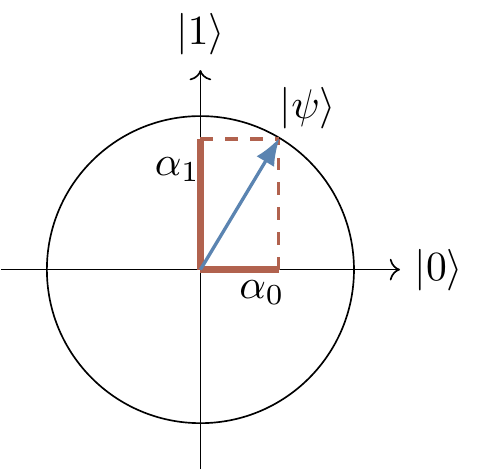
\includegraphics{quantum-info_files/figure-latex/standard-basis-measurement-1} 

}

\caption{The standard (computational) basis defines the standard measurements.}\label{fig:standard-basis-measurement}
\end{figure}

However, if we want to emphasise the role of the measurement, then we can include it explicitly in the diagram as a special quantum gate, e.g.~as

\begin{center}\includegraphics{quantum-info_files/figure-latex/unnamed-chunk-28-1} \end{center}

or, in an alternative notation, as

\begin{center}\includegraphics{quantum-info_files/figure-latex/unnamed-chunk-29-1} \end{center}

As we can see, if the qubit is prepared in state \(|\psi\rangle = \alpha_0|0\rangle + \alpha_1|1\rangle\) and subsequently measured in the standard basis state, then the outcome is \(|k\rangle\) (for \(k=0,1\)) with probability\footnote{This slick argument is a good example of how nice the bra-ket notation can be.}
\[
  \begin{aligned}
    |\alpha_k|^2
    &= |\langle k|\psi\rangle|^2
  \\&= \underbrace{\langle\psi|k\rangle}_{\alpha_k^\star}
    \underbrace{\langle k|\psi\rangle}_{\alpha_k}
  \\&= \langle\psi| \underbrace{|k\rangle\langle k|}_{\text{projector}} |\psi\rangle
  \\&= \langle\psi|P_k|\psi\rangle
  \end{aligned}
\]
where \(P_k=|k\rangle\langle k|\) is the projector on \(|k\rangle\).
If the outcome of the measurement is \(k\), then the output state of the measurement gate is \(|k\rangle\).
The original state \(|\psi\rangle\) is \emph{irretrievably lost}.
This sudden change of the state, from the pre-measurement state \(|\psi\rangle\) to the post-measurement state, either \(|0\rangle\) or \(|1\rangle\), is often called a \textbf{collapse} or a \textbf{reduction} of the state.

So it looks like there are two distinct ways for a quantum state to change: on the one hand we have unitary evolutions, and on the other hand we have an abrupt change during the measurement process.
Surely, the measurement process is not governed by any different laws of physics?

No, it is not!

A measurement is a physical process and can be explained without any ``collapse'', but it is usually a complicated process in which one complex system (a measuring apparatus or an observer) interacts and gets correlated with a physical system being measured.
We will discuss this more later on, but for now let us accept a ``collapse'' as a \emph{convenient mathematical shortcut}, and describe it in terms of projectors rather than unitary operators.

\hypertarget{the-projection-rule-incomplete-measurements}{%
\subsection{The projection rule; incomplete measurements}\label{the-projection-rule-incomplete-measurements}}

So far we have identified measurements with orthonormal bases, or, if you wish, with a set of orthonormal projectors on the basis vectors.

\begin{idea}

\begin{itemize}
\tightlist
\item
  The \textbf{orthonormality} condition:
  \[
      \langle e_k|e_l\rangle = \delta_{kl}
    \]
  i.e.~the basis consists of unit vectors that are pairwise orthogonal.
\item
  The \textbf{completeness} condition:
  \[
      \sum_k|e_k\rangle\langle e_k| = \operatorname{id}
    \]
  i.e.~\emph{any} vector in \(\mathcal{H}\) can be expressed as the sum of orthogonal projections on \(|e_k\rangle\).
\end{itemize}

\end{idea}

Given a quantum system in state \(|\psi\rangle\) such that \(|\psi\rangle = \sum_k \alpha_k|e_k\rangle\), we can write
\[
  \begin{aligned}
    |\psi\rangle
    &= \operatorname{id}|\psi\rangle
  \\&= \sum_k |e_k\rangle\langle e_k| |\psi\rangle
  \\&= \sum_k |e_k\rangle\langle e_k|\psi\rangle
  \\&= \sum_k |e_k\rangle\alpha_k
  \\&= \sum_k \alpha_k|e_k\rangle.
  \end{aligned}
\]
This says that the measurement in the basis \(\{|e_i\rangle\}\) gives the outcome labelled by \(e_k\) with probability
\[
  |\langle e_k|\psi\rangle|^2 = \langle\psi|e_k\rangle\langle e_k|\psi\rangle
\]
and leaves the system in state \(|e_k\rangle\).
This is a \emph{complete} measurement, which represents the best we can do in terms of resolving state vectors in the basis states.
But sometimes we do not want our measurement to distinguish all the elements of an orthonormal basis.

For example, a complete measurement in a four-dimensional Hilbert space will have four distinct outcomes: \(|e_1\rangle\), \(|e_2\rangle\), \(|e_3\rangle\), and \(|e_4\rangle\), but we may want to lump together some of the outcomes and distinguish, say, only between \(\{|e_1\rangle\), \(|e_2\rangle\}\), and \(\{|e_3\rangle,|e_4\rangle\}\).
In other words, we might be trying to distinguish one \emph{subspace} from another, without separating vectors that lie in the same subspace.
Such measurements (said to be \textbf{incomplete}) are indeed possible, and they can be less disruptive than the complete measurements.

\begin{idea}

Intuitively, an incomplete measurement has fewer outcomes and is hence less informative, but the state after such a measurement is usually less disturbed.

\end{idea}

In general, instead of projecting on one dimensional subspaces spanned by vectors from an orthonormal basis, we can decompose our Hilbert space into mutually orthogonal subspaces of various dimensions and project on them.

\begin{idea}

\begin{itemize}
\tightlist
\item
  The orthogonality conditions for projectors:
  \[
      P_k P_l = P_k\delta_{kl}
    \]
\item
  The projector decomposition of the identity:
  \[
      \sum_k P_k = \operatorname{id}
    \]
\end{itemize}

\end{idea}

For any decomposition of the identity into orthogonal projectors \(P_k\), there exists a measurement that takes a quantum system in state \(|\psi\rangle\), outputs label \(k\) with probability \(\langle\psi|P_k|\psi\rangle\), and leaves the system in the state \(P_k|\psi\rangle\) (multiplied by the normalisation factor, i.e.~divided by the length of \(P_k|\psi\rangle\)):
\[
  |\psi\rangle
  \mapsto
  \frac{P_k|\psi\rangle}{\sqrt{\langle\psi|P_k|\psi\rangle}}.
\]

\hypertarget{example-of-an-incomplete-measurement}{%
\subsection{Example of an incomplete measurement}\label{example-of-an-incomplete-measurement}}

Consider a three-dimensional Hilbert space \(\mathcal{H}\), and the two orthogonal projectors
\[
  \begin{aligned}
    P &= |e_1\rangle\langle e_1| + |e_2\rangle\langle e_2|
  \\Q &= |e_3\rangle\langle e_3|
  \end{aligned}
\]
that form the decomposition of the identity: \(P+Q=\operatorname{id}\).
Suppose that a physical system is prepared in state \(|\psi\rangle = \alpha_1|e_1\rangle + \alpha_2|e_2\rangle + \alpha_3|e_3\rangle\).
Ideally, we would like to perform a complete measurement that would resolve the state \(|v\rangle\) into the three basis states, but suppose our experimental apparatus is not good enough, and lumps together \(|e_1\rangle\) and \(|e_2\rangle\).
In other words, it can only differentiate between the two subspaces associated with projectors \(P\) and \(Q\).

The apparatus, in this incomplete measurement, may find the system in the subspace associated with \(P\).
This happens with probability
\[
  \begin{aligned}
    \langle\psi|P|\psi\rangle
    &= \langle\psi|e_1\rangle \langle e_1|\psi\rangle + \langle\psi|e_2\rangle \langle e_2|\psi\rangle
  \\&= |\alpha_1|^2 + |\alpha_2|^2,
  \end{aligned}
\]
and the state right after the measurement is the normalised vector \(P|\psi\rangle\), i.e.
\[
  \frac{\alpha_1|e_1\rangle+\alpha_2|e_2\rangle}{\sqrt{|\alpha_1|^2 + |\alpha_2|^2}}.
\]

The measurement may also find the system in the subspace associated with \(Q\) with the probability \(\langle\psi|Q|\psi\rangle = |\alpha_3|^2\), resulting in the post-measurement state \(|e_3\rangle\).

\begin{center}\includegraphics{quantum-info_files/figure-latex/unnamed-chunk-30-1} \end{center}

\hypertarget{observables}{%
\subsection{Observables}\label{observables}}

An \textbf{observable} \(A\) is a measurable physical property which has a numerical value, for example, spin or momentum or energy.
The term ``observable'' also extends to any basic measurement in which each outcome is associated with a numerical value.
If \(\lambda_k\) is the numerical value associated with outcome \(|e_k\rangle\) then we say that the observable \(A\) is \textbf{represented} by the operator
\[
  \begin{aligned}
    A
    &= \sum_k \lambda_k |e_k\rangle\langle e_k|
  \\&= \sum_k \lambda_k P_k,
  \end{aligned}
\]
where \(\lambda_k\) is now the eigenvalue corresponding to the eigenvector \(|e_k\rangle\), or the projector \(P_k\).

\begin{idea}

Recall the following types of operator:

\begin{longtable}[]{@{}ll@{}}
\toprule
\endhead
\textbf{normal} & \(AA^\dagger = A^\dagger A\)\tabularnewline
\textbf{unitary} & \(AA^\dagger = A^\dagger A = \operatorname{id}\)\tabularnewline
\textbf{Hermitian}, or \textbf{self-adjoint} & \(A^\dagger = A\)\tabularnewline
\textbf{positive semi-definite} & \(\langle v|A|v\rangle\geqslant 0\) for all \(|v\rangle\)\tabularnewline
\bottomrule
\end{longtable}

Note that an operator \(A\) is normal if and only if it is unitarily diagonalisable, and that both unitary and Hermitian operators are normal.

\end{idea}

Conversely, to any normal operator \(A\) we can associate a measurement defined by the eigenvectors of \(A\), which form an orthonormal basis, and use the eigenvalues of \(A\) to label the outcomes of this measurement.
If we choose the eigenvalues to be real numbers then \(A\) becomes a Hermitian operator.
For example, the standard measurement on a single qubit is often called the \textbf{\(Z\)-measurement}, because the Pauli \(Z\) operator can be diagonalised in the standard basis and written as \(Z = (+1)|0\rangle\langle 0| + (-1)|1\rangle\langle 1|\).
The two outcomes, \(|0\rangle\) and \(|1\rangle\), are now labelled as \(+1\) and \(-1\), respectively.
Using the same association we also have the \(X\)- and the \(Y\)-measurements, defined by the Pauli \(X\) and \(Y\) operators, respectively.

Let us mention in passing that many textbooks describe observables in terms of Hermitian operators and claim that the corresponding operators have to be Hermitian ``because the outcomes are real numbers''.
This is misleading, since:

\begin{idea}

The outcomes can be labelled by any symbols of your choice; it is the \emph{decomposition} of the Hilbert space into \emph{mutually orthogonal subspaces} that defines a measurement, not the labels.

\end{idea}

This said, labelling outcomes with real numbers is very useful.
For example, the expected value \(\langle A\rangle\), which is the average of the numerical values \(\lambda_k\) weighted by their probabilities, is a very useful quantity and can be easily expressed in terms of the operator \(A\) as \(\langle\psi|A|\psi\rangle\), as follows:
\[
  \begin{aligned}
    \sum_k \lambda_k \Pr (\text{outcome k})
    &= \sum_k \lambda_k |\langle e_k|\psi\rangle|^2
  \\&= \sum_k\lambda_k \langle\psi|e_k\rangle\langle e_k|\psi\rangle
  \\&= \langle\psi| \left( \sum_k\lambda_k|e_k\rangle\langle e_k| \right)|\psi\rangle
  \\&= \langle\psi|A|\psi\rangle.
  \end{aligned}
\]
To be clear, this is not a value we expect to see in any particular experiment.
Instead, imagine a huge number of quantum objects, all prepared in the state \(|\psi\rangle\) and think about the observable \(A\) being measured on each of the objects.
Statistically we then expect the average of our measurement results to be roughly \(\langle A\rangle\).
Note that when \(A\) is a projector then \(\langle\psi|A|\psi\rangle\) is the probability of the outcome associated with \(A\).

\hypertarget{compatible-observables-and-the-uncertainty-relation}{%
\subsection{Compatible observables and the uncertainty relation}\label{compatible-observables-and-the-uncertainty-relation}}

\textbf{!!!TODO!!!}

\hypertarget{quantum-communication}{%
\subsection{Quantum communication}\label{quantum-communication}}

Now is a good moment to introduce Alice and Bob (not their real names): our two protagonists who always need to communicate with each other.
These two play the major role in many communication dramas, though they remain rather lacking in character development.

This time Alice is sending quantum states to Bob, and Bob does his best to identify them correctly by choosing appropriate measurements.
Let us start we a simple observation: if a quantum state of the carrier of information is described by a state vector in a \(2^n\)-dimensional Hilbert space, then the carrier can carry at most \(n\) bits of information.
For example, Alice can choose one of the \(2^n\) states from a pre-agreed orthonormal basis \(\{|e_k\rangle\}\), and Bob will be able to distinguish them reliably by choosing the \(\{|e_k\rangle\}\) basis for his measurement.

But can Alice and Bob do better than that?
Can Alice send more than \(n\) bits of information per carrier by encoding them in states \(|s_1\rangle,\ldots,|s_N\rangle\) where \(N \geqslant 2^n\)?
Can Bob choose a clever measurement and reliably distinguish between all such states?

The answer is \emph{no}.

\hypertarget{basic-quantum-coding-and-decoding}{%
\subsection{Basic quantum coding and decoding}\label{basic-quantum-coding-and-decoding}}

Suppose Alice randomly chooses one of the pre-agreed \(N\) signal states \(|s_k\rangle\) and sends it to Bob, who tries to identify the signal states by performing a measurement defined by the projectors \(P_l\).
Let \(P\) be a projector on a subspace spanned by the signal states \(|e_k\rangle\), i.e.~\(P|s_k\rangle = |s_k\rangle\).
The dimension \(d\) of this subspace is given by \(d = \operatorname{tr}P\).
We shall assume, without any loss of generality, that Bob designed his measurement in such a way that, whenever he gets outcome \(P_k\), he concludes that Alice sent state \(|s_k\rangle\).
His probability of success is given by
\[
  \Pr(\mbox{success})
  = \frac{1}{N} \sum_k \langle s_k|P_k|s_k\rangle
\]
which is the probability that signal state \(|s_k\rangle\) is selected (here equal to \(1/N\), since all the signal states are equally likely) times the probability that the selected signal state is correctly identified by Bob (which is \(\langle s_k|P_k|s_k\rangle\)), and we sum over all signal states.

\begin{idea}

We have the following \textbf{trace identities}:

\begin{itemize}
\tightlist
\item
  \(\operatorname{tr}(ABC) = \operatorname{tr}(BCA) = \operatorname{tr}(CAB)\)
\item
  \(\operatorname{tr}|a\rangle\langle b| = \langle b|a\rangle\)
\item
  \(\operatorname{tr}|a\rangle\langle b| = \langle b|A|a\rangle\)
\item
  \(\operatorname{tr}BP \leqslant\operatorname{tr}B\) for any positive semi-definite \(B\) and projector \(P\).
\end{itemize}

To prove this last identity, consider the projector \(Q=\operatorname{id}-P\), and note that
\[
  \begin{aligned}
    \operatorname{tr}B
    &= \operatorname{tr}B(P+Q)
  \\&= \operatorname{tr}BP + \operatorname{tr}BQ
  \end{aligned}
\]
and that \(\operatorname{tr}BQ\) is non-negative.

\end{idea}

Let us use this case to practice some of the trace identities.
It is often convenient to write expressions such as \(\langle\psi|A|\psi\rangle\) in terms of the trace: for any vector \(|\psi\rangle\) and operator \(A\) we have
\[
  \begin{aligned}
    \langle\psi|A|\psi\rangle
    &= \operatorname{tr}(A|\psi\rangle\langle\psi|)
  \\&= \operatorname{tr}(|\psi\rangle\langle\psi| A).
  \end{aligned}
\]
In our case,
\[
  \begin{aligned}
    \Pr(\mbox{success})
    &= \frac{1}{N} \sum_k \langle s_k|P_k|s_k\rangle
  \\&= \frac{1}{N} \sum_k \langle s_k|PP_kP|s_k\rangle
  \\&= \frac{1}{N} \sum_k \operatorname{tr}(PP_kP) |s_k\rangle\langle s_k|
  \end{aligned}
\]
where we have also used that \(P|s_k\rangle=|s_k\rangle\).
Let us bound this expression above by using the trace identities:
\[
  \begin{aligned}
    \frac{1}{N} \sum_k \operatorname{tr}(PP_kP) |s_k\rangle\langle s_k|
    &\leqslant\frac{1}{N} \sum_k \operatorname{tr}(PP_kP)
  \\&= \frac{1}{N} \sum_k \operatorname{tr}\left( P\left( \sum_k P_k \right) P \right)
  \\&= \frac{1}{N} \sum_k \operatorname{tr}(P\operatorname{id}P)
  \\&= \frac{d}{N}
  \end{aligned}
\]

So if Alice encodes \(N\) equally likely messages as states in a quantum system that, mathematically speaking, lives in the Hilbert space of dimension \(d\), and if Bob decodes by performing a measurement and inferring the message from the result, then Bob's probability of success is bounded by \(\frac{d}{N}\).
If the number \(N\) of possible signals exceeds the dimension \(d\), then Bob will not be able to reliably distinguish between the signals by any measurement.
In particular:

\begin{idea}

One qubit can store and carry \emph{at most} one bit of information that can \emph{reliably} be read by a measurement.

\end{idea}

\hypertarget{distinguishability-of-non-orthogonal-states}{%
\subsection{Distinguishability of non-orthogonal states}\label{distinguishability-of-non-orthogonal-states}}

We have already mentioned that non-orthogonal states cannot be reliably distinguished, and now it is time to make this statement more precise.
Suppose Alice sends Bob a message by choosing one of the two non-orthogonal states \(|s_1\rangle\) and \(|s_2\rangle\), where both are equally likely to be chosen.
What is the probability that Bob will decode the message correctly and what is the best (i.e.~the one that maximises this probability) measurement?
As a general rule, before you embark on any calculations, check for symmetries, special cases, and anything that may help you to visualise the problem and make intelligent guesses about the solution.
One of the most powerful research tools is a good guess.
In fact, this is what real research is about: educated guesses that guide your calculations.
In this particular case you can use symmetry arguments to guess the optimal measurement --- see Figure \ref{fig:optimal-measurement}.
Once you have guessed the answer, you might as well do the calculations.



\begin{figure}[H]

{\centering \includegraphics{quantum-info_files/figure-latex/optimal-measurement-1} 

}

\caption{The optimal measurement to distinguish between the two equally likely non-orthogonal signal states \(|s_1\rangle\) and \(|s_2\rangle\) is described by the two orthogonal vectors \(|d_1\rangle\) and \(|d_2\rangle\) placed symmetrically around the signal states.}\label{fig:optimal-measurement}
\end{figure}

Suppose Bob's measurement is described by projectors \(P_1\) and \(P_2\), with the inference rule ``\(P_1\) implies \(|s_1\rangle\); \(P_2\) implies \(|s_2\rangle\)''.
Then
\[
  \begin{aligned}
    \Pr(\mbox{success})
    &= \frac12\left(
        \langle s_1|P_1|s_1\rangle + \langle s_2|P_2|s_2\rangle
      \right)
  \\&= \frac12\left(
        \operatorname{tr}P_1|s_1\rangle\langle s_1| + \operatorname{tr}P_2|s_2\rangle\langle s_2|
      \right)
  \\&= \frac12\left(
        \operatorname{tr}P_1|s_1\rangle\langle s_1| + \operatorname{tr}(\operatorname{id}-P_1)|s_2\rangle\langle s_2|
      \right)
  \\&= \frac12\left(
        1 + \operatorname{tr}P_1\left( |s_1\rangle\langle s_1| - |s_2\rangle\langle s_2| \right)
      \right).
\end{aligned}
\]
Let us look at the operator \(D = |s_1\rangle\langle s_1| - |s_2\rangle\langle s_2|\) that appears in the last expression.
This operator acts on the subspace spanned by \(|s_1\rangle\) and \(|s_2\rangle\); it is Hermitian; the sum of its two (real) eigenvalues is zero; and \(\operatorname{tr}D=\langle s_1\rangle{s_1}-\langle s_2\rangle{s_2}=0\).
Let us write \(D\) as \(\lambda(|d_+\rangle\langle d_+| - |d_-\rangle\langle d_-|)\), where \(|d_\pm\rangle\) are the two orthonormal eigenstates of \(D\), and \(\pm\lambda\) are the corresponding eigenvalues.
Now we write
\[
\begin{aligned}
  \Pr (\mbox{success})
  &= \frac12\left(
      1 + \lambda\operatorname{tr}P_1\left( |d_+\rangle\langle d_+|-|d_-\rangle\langle d_-| \right)
    \right)
\\&\leqslant\frac12\left(
      1+\lambda \langle d_+|P_1|d_+\rangle
    \right)
\end{aligned}
\]
where we have dropped the non-negative term \(\operatorname{tr}P_1|d_-\rangle\!\langle d_-|\).
In fact, it is easy to see that we will maximise the expression above by choosing \(P_1 = |d_+\rangle\langle d_+|\) (and \(P_2 = |d_-\rangle\langle d_-|\)).
The probability of success is then bounded by \(\frac12(1+\lambda)\).
All we have to do now is to find the positive eigenvalue \(\lambda\) for the operator \(D\).
We can do this, of course, by solving the characteristic equation for a matrix representation of \(D\), but, as we are now practising the trace operations, we can also notice that \(\operatorname{tr}D^2 = 2\lambda^2\), and then evaluate the trace of \(D^2\).
We use the trace identities and obtain
\[
  \begin{aligned}
    \operatorname{tr}D^2
    &= \operatorname{tr}\left( |s_1\rangle\langle s_1|-|s_2\rangle\langle s_2| \right) \left( |s_1\rangle\langle s_1|-|s_2\rangle\langle s_2| \right)
  \\&= 2-2|\langle s_1|s_2\rangle|^2
  \end{aligned}
\]
which gives \(\lambda = \sqrt{1-|\langle s_1|s_2\rangle|^2}\).
Bringing it all together we have the final expression:
\[
 \Pr (\mbox{success})
 = \frac12\left( 1+ \sqrt{1-|\langle s_1|s_2\rangle|^2} \right).
\]

We can parametrise \(|\langle s_1|s_2\rangle| = \cos\alpha\), and interpret \(\alpha\) as the angle between \(|s_1\rangle\) and \(|s_2\rangle\).

\begin{center}\includegraphics{quantum-info_files/figure-latex/unnamed-chunk-31-1} \end{center}

This allows us to express our findings in a clearer way: given two equally likely states, \(|s_1\rangle\) and \(|s_2\rangle\), such that \(|\langle s_1|s_2\rangle| = \cos\alpha\), the probability of correctly identifying the state by a projective measurement is bounded by
\[
 \Pr (\mbox{success})
 = \frac12(1 + \sin\alpha),
\]
and the optimal measurement that achieves this bound is determined by the eigenvectors of \(D = |s_1\rangle\langle s_1|-|s_2\rangle\langle s_2|\) (try to visualise these eigenvectors).

It makes sense, right?
If we try just guessing the state, without any measurement, then we expect \(\Pr (\mbox{success}) = \frac12\).
This is our lower bound, and in any attempt to distinguish the two states we should do better than that.
If the two signal states are very close to each other then \(\sin\alpha\) is small and we are slightly better off than guessing.
As we increase \(\alpha\), the two states become more distinguishable, and, as we can see from the formula, when the two states become orthogonal they also become completely distinguishable.

\hypertarget{wiesners-quantum-money}{%
\subsection{Wiesner's quantum money}\label{wiesners-quantum-money}}

\textbf{!!!TODO!!!}

\hypertarget{exercises-6}{%
\subsection{Exercises}\label{exercises-6}}

\begin{enumerate}
\def\labelenumi{\arabic{enumi}.}
\item
  Consider two unit vectors \(|a\rangle\) and \(|b\rangle\).
  Is \(|a\rangle\langle a|+|b\rangle\langle b|\) a projector?
  2.Suppose you are given a single qubit in some unknown quantum state \(|\psi\rangle\).
  Can you determine \(|\psi\rangle\)?
\item
  You measure a random qubit in the standard basis and register \(|0\rangle\).
  What does it tell you about the pre-measurement state \(|\psi\rangle\)?
\item
  How many real parameters do you need to determine \(|\psi\rangle\)?
  Would you be able to reconstruct \(|\psi\rangle\) from \(\langle\psi|X|\psi\rangle\), \(\langle\psi|Y|\psi\rangle\), and \(\langle\psi|Z|\psi\rangle\)?
  (It may help you to visualise \(|\psi\rangle\) as a Bloch vector).
\item
  You are given zillions of qubits, all prepared in the same quantum state \(|\psi\rangle\).
  How would you determine \(|\psi\rangle\)?
\item
  The \(Z\) measurement is defined by the projectors
  \[
     \begin{aligned}
       P_0 &= \frac12(\operatorname{id}+ Z),
     \\P_1 &= \frac12(\operatorname{id}- Z).
     \end{aligned}
   \]
  Consider the measurement associated to some Hermitian operator \(S\) that satisfies \(S^2=\operatorname{id}\).
  Show that the two outcomes \(\pm 1\) correspond to the projectors \(\frac12(\operatorname{id}\pm S)\).
\item
  In our quantum circuits, unless specified otherwise, all measurements are assumed to be performed in the standard basis.
  This is because any measurement can be reduced to the standard measurement by performing some prior unitary transformation.
  Show that any two orthonormal bases \(\{|e_k\rangle\}\) and \(\{|d_l\rangle\}\) are always related by some unitary \(U\) (i.e.~show that \(\sum_k |d_k\rangle\langle e_k|\) is unitary).

  Suppose projectors \(P_k\) define the standard measurement, and show that for any unitary \(U\) projectors \(UP_kU^\dagger\) also define a measurement.
\end{enumerate}

\begin{center}\includegraphics{quantum-info_files/figure-latex/unnamed-chunk-32-1} \end{center}

\begin{enumerate}
\def\labelenumi{\arabic{enumi}.}
\setcounter{enumi}{7}
\tightlist
\item
  The optimal measurement to distinguish between the two equally likely non-orthogonal signal states, \(|s_1\rangle\) and \(|s_2\rangle\), is described by the two orthogonal vectors \(|d_1\rangle\) and \(|d_2\rangle\), placed symmetrically around the signal states.
  But suppose the states are not equally likely: say \(|s_1\rangle\) is chosen with probability \(p_1\) and \(|s_2\rangle\) with probability \(p_2\).
  How would you modify the measurement to maximise the probability of success in this case?
\end{enumerate}

\begin{center}\includegraphics{quantum-info_files/figure-latex/unnamed-chunk-33-1} \end{center}

\begin{enumerate}
\def\labelenumi{\arabic{enumi}.}
\setcounter{enumi}{8}
\tightlist
\item
  (\textbf{How to ascertain the values of \(\sigma_x\) and \(\sigma_y\) of a qubit}).\footnote{This is a simplified version of a beautiful quantum puzzle proposed in 1987 by Lev Vaidman, Yakir Aharonov, and David Z. Albert in a paper with the somewhat provocative title ``How to ascertain the values of \(\sigma_x\), \(\sigma_y\), and \(\sigma_z\) of a spin-\(\frac12\) particle''. For the original, see \emph{Phys. Rev.~Lett.} \textbf{58} (1987), 1385.}
  Alice prepares a qubit in any state of her choosing and gives it to Bob, who secretly measures either \(\sigma_x\) or \(\sigma_y\).
  The outcome of the measurement is seen only by Bob.
  Alice has no clue which measurement was chosen by Bob, but right after his measurement she gets her qubit back and she can measure it as well.
  Some time later, Bob tells Alice which of the two measurements was chosen, i.e.~whether he measured \(\sigma_x\) or \(\sigma_y\).
  Alice then tells him the outcome he obtained in his measurement.
  Bob is surprised, since the two measurements have mutually unbiased bases and yet Alice always gets it right.
  How does she do it?
\item
  (\textbf{Zeno effect}).
  \textbf{!!!TODO!!!}
\end{enumerate}

\hypertarget{quantum-theory-formally}{%
\subsection{Quantum theory, formally}\label{quantum-theory-formally}}

Even though multiplying and adding probability amplitudes is essentially all there is to quantum theory, we hardly ever multiply and add amplitudes in a pedestrian way.
Instead, as we have seen, we neatly tabulate the amplitudes into vectors and matrices and let the matrix multiplication take care of multiplication and addition of amplitudes corresponding to different alternatives.
Thus vectors and matrices appear naturally as our bookkeeping tools: we use vectors to describe quantum states, and matrices (operators) to describe quantum evolutions and measurements.
This leads to a convenient mathematical setting for quantum theory, which is a complex vector space with an inner product, often referred to as a Hilbert space.
It turns out, somewhat miraculously, that this pure mathematical construct is exactly what we need to formalise quantum theory.
It gives us a precise language which is appropriate for making empirically testable predictions.
At a very instrumental level, quantum theory is a set of rules designed to answer questions such as ``given a specific preparation and a subsequent evolution, how can we compute probabilities for the outcomes of such-and-such measurement''.
Here is how we represent preparations, evolutions and measurements in mathematical terms, and how we get probabilities.

Note that we have already said much of the below, but we are summarising it again now in a more precise way, formally defining the mathematical framework of quantum theory that we use.

We also need to point out that a vital part of the formalism of quantum theory is missing from the following description, namely the idea of \textbf{tensor products}.
To talk about this, we need to introduce the notion of \textbf{entanglement}, and this will be the subject of \protect\hyperlink{chapter5}{Chapter 5}.

\hypertarget{quantum-states}{%
\subsubsection{Quantum states}\label{quantum-states}}

With any isolated quantum system which can be prepared in \(n\) perfectly distinguishable states, we can associate a Hilbert space \(\mathcal{H}\) of dimension \(n\) such that each vector \(|v\rangle\in\mathcal{H}\) of unit length (\(\langle v|v\rangle =1\)) represents a quantum state of the system.
The overall phase of the vector has no physical significance: \(|v\rangle\) and \(e^{i\varphi}|v\rangle\), for any real \(\varphi\), describe the same state.
The inner product \(\langle u|v\rangle\) is the probability amplitude that a quantum system prepared in state \(|v\rangle\) will be found in state \(|u\rangle\).
States corresponding to orthogonal vectors, \(\langle u|v\rangle=0\), are perfectly distinguishable, since the system prepared in state \(|v\rangle\) will never be found in state \(|u\rangle\), and vice versa.
In particular, states forming orthonormal bases are always perfectly distinguishable from each other.

\hypertarget{quantum-evolutions}{%
\subsubsection{Quantum evolutions}\label{quantum-evolutions}}

\begin{idea}

Any physically admissible evolution of an isolated quantum system is represented by a unitary operator.

\end{idea}

Unitary operators describing evolutions of quantum systems are usually derived from the \textbf{Schrödinger equation}.\footnote{Recall our \protect\hyperlink{quantum-dynamics}{previous discussion} of this equation.}
\[
  \frac{\mathrm{d}}{\mathrm{d}t} |\psi(t)\rangle
  = -\frac{i}{\hbar} H |\psi(t)\rangle
\]
where \(H\) is a Hermitian operator called the Hamiltonian.

This equation contains a complete specification of all interactions both within the system and between the system and the external potentials.
For time independent Hamiltonians, the formal solution of the Schrodinger equation reads
\[
  \begin{gathered}
    |\psi(t)\rangle = U(t) |\psi(0)\rangle
  \\\mbox{where}\qquad
    U(t) = e^{-\frac{i}{\hbar}Ht}.
  \end{gathered}
\]
Any unitary matrix can be represented\footnote{We ignore convergence issues.} as the exponential of some Hermitian matrix \(H\) and some real coefficient \(t\)
\[
  \begin{aligned}
    e^{i t H}
    &\equiv \operatorname{id}+ itH + \frac{(it)^2}{2}H^2 + \frac{(it)^3}{2\cdot3}H^3 +\ldots
  \\&= \sum_{n=0}^\infty \frac{(it)^n}{n!}H^n.
  \end{aligned}
\]
The state vector changes smoothly: for \(t=0\) the time evolution operator is merely the unit operator \(\operatorname{id}\), and when \(t\) is very small \(U(t)\approx \operatorname{id}-itH\) is close to the unit operator, differing from it by something of order \(t\).

\hypertarget{quantum-circuits}{%
\subsubsection{Quantum circuits}\label{quantum-circuits}}

In this course we will hardly refer to the Schrödinger equation.
Instead we will assume that our clever colleagues, experimental physicists, are able to implement certain unitary operations and we will use these unitaries, like lego blocks, to construct other, more complex, unitaries.
We refer to preselected elementary quantum operations as \textbf{quantum logic gates} and we often draw diagrams, called \textbf{quantum circuits}, to illustrate how they act on qubits.
For example, two unitaries, \(U\) followed by \(V\), acting on a single qubit are represented as

\begin{center}\includegraphics{quantum-info_files/figure-latex/unnamed-chunk-34-1} \end{center}

This diagram should be read from left to right, and the horizontal line represents a qubit that is inertly carried from one quantum operation to another.

\hypertarget{measurements}{%
\subsubsection{Measurements}\label{measurements}}

A complete measurement in quantum theory is determined by the choice of an orthonormal basis \(\{|e_i\rangle\}\) in \(\mathcal{H}\), and every such basis (in principle) represents a possible measurement.
Given a quantum system in state \(|\psi\rangle\) such that
\[
  |\psi\rangle = \sum_i |e_i\rangle\langle e_i|\psi\rangle,
\]
the measurement in the basis \(\{|e_i\rangle\}\) gives the outcome labelled by \(e_k\) with probability \(|\langle e_k\psi\rangle|^2\), and leaves the system in state \(|e_k\rangle\).
This is consistent with our interpretation of the inner product \(\langle e_k|\psi\rangle\) as the probability amplitude that a quantum system prepared in state \(|\psi\rangle\) will be found in state \(|e_k\rangle\).
State vectors forming orthonormal bases are perfectly distinguishable from each other (\(\langle e_i|e_j\rangle=\delta_{ij}\)), so there is no ambiguity about the outcome.
A complete measurement is the best we can do in terms of resolving state vectors in the basis states.

In general, for any decomposition of the identity \(\sum_k P_k=\operatorname{id}\) into orthogonal projectors \(P_k\) (i.e.~\(P_kP_l = P_k\delta_{kl}\)), there exists a measurement that takes a quantum system in state \(|\psi\rangle\), outputs label \(k\) with probability \(\langle\psi|P_k|\psi\rangle\), and leaves the system in the state \(P_k|\psi\rangle\) (multiplied by the normalisation factor i.e.~divided by the length of \(P_k|\psi\rangle\)):
\[
  |\psi\rangle
  \mapsto
  \frac{P_k|\psi\rangle}{\sqrt{\langle\psi|P_k|\psi\rangle}}.
\]
The projector formalism covers both complete and incomplete measurements.
The complete measurements are defined by rank one projectors, \(P_k=|e_k\rangle\langle e_k|\), projecting on vectors from some orthonormal basis \(\{|e_k\rangle\}\).

\hypertarget{chapter5}{%
\section{Quantum entanglement}\label{chapter5}}

\begin{quote}
On \ldots{} \textbf{!!!TODO!!!}
\end{quote}

We now know everything we need to know about a single qubit and its quantum behaviour.
But if we want to understand quantum computation --- a complicated quantum interference of many interacting qubits --- then we will need few more mathematical tools.
Stepping up from one qubit to two or more is a bigger leap than you might expect.
Already, with just two qubits, we will encounter the remarkable phenomenon of quantum entanglement and have a chance to discuss some of the most puzzling features of quantum theory that took people decades to understand.

\hypertarget{a-small-history}{%
\subsection{A small history}\label{a-small-history}}

The notion of \textbf{quantum entanglement} was the subject of many early debates that focused on the meaning of quantum theory.
Back in the 1930s, Albert Einstein, Niels Bohr, Werner Heisenberg, and Erwin Schrodinger (to mention just the usual suspects) were trying hard to understand its conceptual consequences.\footnote{E. Schrodinger, Discussion of probability relations between separated system, \emph{Mathematical Proceedings of the Cambridge Philosophical Society} \textbf{31} (1935), pp.~555--563.}
Einstein, the most sceptical of them all, claimed that it was pointing toward the fatal flaw in quantum theory, and referred to it as ``\emph{spooky action-at-a-distance}''.
In contrast, Schrödinger was much more prepared to accept quantum theory exactly as it was formulated, along with all its predictions, no matter how weird they might be.
In his 1935 paper, which introduced quantum entanglement, he wrote ``I would not call it \emph{one} but rather \emph{the} characteristic trait of quantum mechanics, the one that enforces its entire departure from classical lines of thought''.
Today we still talk a lot about quantum entanglement, but more often it is viewed as a physical resource which enables us to communicate with perfect security, build very precise atomic clocks, and even teleport small quantum objects!
But what exactly is quantum entanglement?

\hypertarget{one-two-many}{%
\subsection{One, two, many\ldots{}}\label{one-two-many}}

In classical physics, the transition from a single object to a composite system of many objects is trivial: in order to describe the state of, say, 42 objects at any given moment of time, it is sufficient to describe the state of each of the objects separately.
Indeed, the classical state of 42 point-like particles is described by specifying the position and the momentum of each particle.

\begin{idea}

In the \emph{classical} world, ``the whole is the sum of its parts'', but the \emph{quantum} world is very different.

\end{idea}

Consider, for example, a pair of qubits.
Suppose that each one is described by a state vector: the first one by \(|a\rangle\), and the second one by \(|b\rangle\).
One might therefore think that the most general state of the two qubits should be represented by a pair of state vectors, \(|a\rangle|b\rangle\), with one for each qubit.
Indeed, such a state is certainly possible, but there are other states that \emph{cannot} be expressed in this form.
In order to write down the most general state of two qubits we first focus on the basis states.

For a single qubit we have been using the standard basis \(\{|0\rangle,|1\rangle\}\).
For two qubits we may choose the following as our standard basis states:\footnote{It looks like we are defining some sort of ``multiplication rule'' for kets here, saying that \(|a\rangle|b\rangle:=|ab\rangle\). This is indeed the case, but to talk about this properly we need to introduce the idea of \textbf{tensor products} (which we do very soon).}
\[
  \begin{array}{cc}
    |00\rangle \equiv |0\rangle|0\rangle
    & |01\rangle \equiv |0\rangle|1\rangle
  \\|10\rangle \equiv |1\rangle|0\rangle
    &|11\rangle \equiv |1\rangle|1\rangle.
  \end{array}
\]
Within each ket, the first symbol refers to the first qubit, and the second to the second, and we have tacitly assumed that we can distinguish the two qubits by their location, or some other means.
Now, the most general state of the two qubits is a normalised linear combination of these four basis states, i.e.~a vector of the form
\[
  |\psi\rangle
  = c_{00}|00\rangle + c_{01}|01\rangle + c_{10}|10\rangle + c_{11}|11\rangle.
\]
Physical interpretation aside, let us count how many real parameters are needed to specify this state.
Six, right?
We have four complex numbers (eight real parameters) restricted by the normalisation condition, along with the fact that states differing only by a global phase factor are equivalent, which leaves us with six real parameters.
Now, by the same line of argument, we need only two real parameters to specify the state of a single qubit, and hence need four real parameters to specify any state of two qubits of the form \(|a\rangle|b\rangle\).
So it cannot be the case that every state of two qubits can be expressed as a pair of states \(|a\rangle|b\rangle\), simply for ``dimension reasons''.

For example, compare the two states of two qubits,
\[
  \begin{gathered}
    \frac{1}{\sqrt 2}|00\rangle + \frac{1}{\sqrt 2}|01\rangle
  \\\mbox{and}
  \\\frac{1}{\sqrt 2}|00\rangle + \frac{1}{\sqrt 2}|11\rangle.
  \end{gathered}
\]
The first one is \textbf{separable}, i.e.~we can view it as a pair of state vectors where each one pertains to one of the two qubits:
\[
  \frac{1}{\sqrt 2}|00\rangle + \frac{1}{\sqrt 2}|01\rangle
  = \underbrace{\vphantom{\frac{1}{\sqrt 2}}|0\rangle}_{\text{qubit 1}}
  \;\;
  \underbrace{\frac{1}{\sqrt 2}(|0\rangle+|1\rangle)}_{\text{qubit 2}},
\]
The second state, however, does \emph{not} admit such a decomposition: there do \emph{not} exist any \(\psi_1,\psi_2\) such that
\[
  \frac{1}{\sqrt 2}|00\rangle + \frac{1}{\sqrt 2}|11\rangle
  =
  |\psi_1\rangle|\psi_2\rangle
\]
and so we say that it is an \textbf{entangled} state.
Informally, any bipartite state that cannot be viewed as a pair of two states pertaining to the constituent subsystems is said to be entangled.

With this discussion in our minds, we can now give more formal account of the states of composite quantum systems.

\hypertarget{quantum-theory-formally-continued}{%
\subsection{Quantum theory, formally (continued)}\label{quantum-theory-formally-continued}}

Recalling \protect\hyperlink{chapter4}{Chapter 4}, where we said that we were missing a key part of the formalism of quantum theory, we can now fill in this hole.
Our mathematical formalism of choice behind the quantum theory of composite systems is based on the \textbf{tensor product} of Hilbert spaces.

\hypertarget{tensor-products}{%
\subsubsection{Tensor products}\label{tensor-products}}

Let the states of some system \(\mathcal{A}\) be described by vectors in an \(n\)-dimensional Hilbert space \(\mathcal H_A\), and the states of some system \(\mathcal{B}\) by vectors in an \(m\)-dimensional Hilbert space \(\mathcal H_B\).
The combined system of \(\mathcal{A}\) and \(\mathcal{B}\) is then described by vectors in the \((nm)\)-dimensional \textbf{tensor product space} \(\mathcal{H}_A\otimes\mathcal{H}_B\).
Given bases \(\{|a_1\rangle,\ldots,|a_n\rangle\}\) of \(\mathcal H_A\) and \(\{|b_1\rangle,\ldots,|b_m\rangle\}\) of \(\mathcal H_B\), we form a basis of the tensor product by taking the ordered pairs \(|a_i\rangle\otimes|b_j\rangle\), for \(i=1,\ldots,n\) and \(j=1,\ldots,m\).
The tensor product space \(\mathcal{H}_A\otimes\mathcal{H}_B\) then consists of all linear combination of such tensor product basis vectors:\footnote{If the bases \(\{|a_i\rangle\}\) and \(\{|b_j\rangle\}\) are orthonormal then so too is the tensor product basis \(\{|a_i\rangle\otimes|b_j\rangle\}\).}
\begin{equation}
  |\psi\rangle
  = \sum_{ij} c_{ij}|a_i\rangle\otimes|b_j\rangle.
\label{eq:bipartite}
\end{equation}

The tensor product operation \(\otimes\) is distributive:
\[
  \begin{gathered}
    |a\rangle \otimes \left( \beta_1|b_1\rangle + \beta_2|b_2\rangle \right)
    = \beta_1|a\rangle\otimes|b_1\rangle + \beta_2|a\rangle\otimes|b_2\rangle
  \\\left( \alpha_1|a_1\rangle + \alpha_2|a_2\rangle \right) \otimes |b\rangle
    = \alpha_1|a_1\rangle\otimes|b\rangle + \alpha_2|a_2\rangle\otimes|b\rangle.
  \end{gathered}
\]
The tensor product of Hilbert spaces is again a Hilbert space: the inner products on \(\mathcal{H}_A\) and \(\mathcal{H}_B\) give a natural inner product on \(\mathcal{H}_A\otimes\mathcal{H}_B\), defined for any two product vectors by\footnote{The bra corresponding to the tensor product state \(|a\rangle\otimes|b\rangle\) is written as \((|a\rangle\otimes|b\rangle)^\dagger = \langle a|\otimes\langle b|\), where the order of the factors on either side of \(\otimes\) does not change when the dagger operation is applied.}
\[
  \left( \langle a'|\otimes\langle b'| \right) \left( |a\rangle\otimes|b\rangle \right)
  = \langle a'|a\rangle\langle b'|b\rangle
\]
and extended by linearity to sums of tensor products of vectors, and by associativity\footnote{\(({\mathcal{H}}_a \otimes {\mathcal{H}}_b)\otimes {\mathcal{H}}_c = {\mathcal{H}}_a \otimes ({\mathcal{H}}_b\otimes {\mathcal{H}}_c)\).} to any number of subsystems.

Some joint states of \(\mathcal{A}\) and \(\mathcal{B}\) can be expressed as a single tensor product, say \(|\psi\rangle=|a\rangle\otimes|b\rangle\) (often written as \(|a\rangle|b\rangle\), or \(|a, b\rangle\), or even \(|ab\rangle\)), meaning that the subsystem \(\mathcal{A}\) is in state \(|a\rangle\), and the subsystem \(\mathcal{B}\) in state \(|b\rangle\).
If we expand \(|a\rangle=\sum_i\alpha_i|a_i\rangle\) and \(|b\rangle=\sum_i\beta_j|b_j\rangle\), then \(|\psi\rangle=\sum_{ij}\alpha_i\beta_j|a_i\rangle\otimes|b_j\rangle\) and we see that, for all such states, the coefficients \(c_{ij}\) in Equation \eqref{eq:bipartite} are of a rather special form:
\[
  c_{ij} = \alpha_i\beta_j.
\]
We call such states \textbf{separable} (or just \textbf{product states}).
States that are not separable are said to be \textbf{entangled}.

A useful fact about tensor products is that \(\lambda a\otimes b = a\otimes\lambda b\) (where \(a\) and \(b\) are vectors, and \(\lambda\) is a scalar).
This means that we don't need to worry about brackets and write something like \(\lambda(a\otimes b)\).

We will also need the concept of the tensor product of two operators.
If \(A\) is an operator on \(\mathcal{H}_A\) and \(B\) an operator on \(\mathcal{H}_B\), then the tensor product operator \(A\otimes B\) is an operator on \(\mathcal{H}_A\otimes\mathcal{H}_B\) defined by its action on product vectors via
\[
  (A\otimes B)(|a\rangle\otimes|b\rangle) = (A|a\rangle)\otimes (B|b\rangle)
\]
and with its action on all other vectors determined by linearity:
\[
  A\otimes B \left( \sum_{ij} c_{ij}|a_i\rangle\otimes|b_j\rangle \right)
  = \sum_{ij}c_{ij} A|a_i\rangle\otimes B|b_j\rangle.
\]

\hypertarget{back-to-qubits}{%
\subsection{Back to qubits}\label{back-to-qubits}}

Let's see how this formalism works for qubits.
The \(n\)-fold tensor product of vectors from the standard basis \(\{|0\rangle,|1\rangle\}\) represent binary strings of length \(n\).
For example, for \(n=3\),\footnote{We often drop the \(\otimes\) symbol, especially when we deal with the standard tensor product basis. For example, a state of a quantum register composed of four qubits holding the binary string \(1001\) may be written as \(|1\rangle\otimes|0\rangle\otimes|0\rangle\otimes|1\rangle\), as \(|1\rangle|0\rangle|0\rangle|1\rangle\), or even simply as \(|1001\rangle\).}
\[
  \begin{aligned}
    |0\rangle\otimes|1\rangle\otimes|1\rangle
    & \equiv |011\rangle
  \\|1\rangle\otimes|1\rangle\otimes|1\rangle
    & \equiv |111\rangle.
  \end{aligned}
\]
A \emph{classical} register composed of three bits can store \emph{only one} of these two binary strings at any time; a \emph{quantum} register composed of three qubits can store \emph{both of them} in a superposition.

Indeed, if we start with the state \(|011\rangle\) and apply the Hadamard gate to the first qubit (which is the same as applying \(H\otimes\operatorname{id}\otimes\operatorname{id}\)), then, given that linear combinations distribute over tensor products, we obtain\footnote{We often simply write \(H\otimes H\otimes H\) as \(H^{\otimes 3}\).}
\[
  \begin{aligned}
    |011\rangle
    \longmapsto
    &\frac{1}{\sqrt2} \big(|0\rangle + |1\rangle\big) \otimes|1\rangle\otimes|1\rangle
  \\\equiv
    &\frac{1}{\sqrt2} \big(|011\rangle + |111\rangle\big).
  \end{aligned}
\]
In fact, we can even prepare this register in a superposition of all eight possible binary strings: if we apply the tensor product operation \(H\otimes H\otimes H\) to the state \(|0\rangle\otimes|0\rangle\otimes|0\rangle = |000\rangle\) then we get

\begin{center}\includegraphics{quantum-info_files/figure-latex/unnamed-chunk-35-1} \end{center}

The resulting state is exactly a superposition of all binary string of length 3, and can also be written as
\[
  \frac{1}{\sqrt2} \big(|0\rangle + |1\rangle\big)
  \otimes
  \frac{1}{\sqrt2} \big(|0\rangle + |1\rangle\big)
  \otimes
  \frac{1}{\sqrt2} \big(|0\rangle + |1\rangle\big).
\]

In general, the tensor product operation \(H^{\otimes n}\), which means ``apply the Hadamard gate to each of your \(n\) qubits'', is known as the \textbf{Hadamard transform}, and it maps product states to product states.
Like the Hadamard gate in the typical quantum interference circuit, the Hadamard transform opens and closes a multi-qubit interference.

\hypertarget{separable-or-entangled}{%
\subsection{Separable or entangled?}\label{separable-or-entangled}}

\begin{idea}

\emph{Most} vectors in \(\mathcal{H}_a\otimes \mathcal{H}_b\) are entangled and \emph{cannot} be written as product states \(|a\rangle\otimes|b\rangle\) with \(|a\rangle\in\mathcal{H}_a\) and \(|b\rangle\in\mathcal{H}_b\).

\end{idea}

In order to see this, let us write any joint state \(|\psi\rangle\) of \(\mathcal{A}\) and \(\mathcal{B}\) in a product basis as
\begin{equation}
  \begin{aligned}
    |\psi\rangle
    &= \sum_{ij} c_{ij}|a_i\rangle\otimes|b_j\rangle
  \\&= \sum_i|a_i\rangle\otimes\left(\sum_j c_{ij}|b_j\rangle\right)
  \\&= \sum_i|a_i\rangle\otimes|\phi_i\rangle
  \end{aligned}
\label{eq:bipartite2}
\end{equation}
where the \(|\phi_i\rangle=\sum_j c_{ij}|b_j\rangle\) are vectors in \(\mathcal{H}_B\) that need not be normalised.
For any \emph{product} state, these vectors have a special form.
Indeed, if \(|\psi\rangle= |a\rangle\otimes|b\rangle\) then, after expanding the first state in the \(|a_i\rangle\) basis, we obtain
\[
  |\psi\rangle
  = \sum_{i}|a_i\rangle\otimes\left(\sum_i\alpha_i|b\rangle\right).
\]
This expression has the same form as Equation \eqref{eq:bipartite2} with \(|\phi_i\rangle=\alpha_i|b\rangle\), i.e.~each of the \(|\phi_i\rangle\) vectors in this expansion is a multiple of the same vector \(|b\rangle\).
Conversely, if \(|\phi_i\rangle = \alpha_i|b\rangle\) for all \(i\) in Equation \eqref{eq:bipartite2}, then \(|\psi\rangle\) must be a product state.\footnote{Even though an entangled state cannot be written as a tensor product, it can always be written as a linear combination of vectors from the tensor product basis. In fact, any state of \(n\) qubits \(|\psi\rangle\) can be expressed in the standard \emph{product} basis. In general, given \(n\) qubits, we need \(2(2^n-1)\) real parameters to describe their state vector, but only \(2n\) to describe separable states.}
So if we want to identify which joint states are product states and which are not, we simply write the joint state according to Equation \eqref{eq:bipartite2} and check if all the vectors \(|\phi_i\rangle\) are multiples of a single vector.
Needless to say, if we choose the states \(|\phi\rangle\) randomly, it is very unlikely that this condition is satisfied, and we almost certainly pick an entangled state.

Quantum entanglement is one of the most fascinating aspects of quantum theory.
We will now explore some of its implications.

\hypertarget{controlled-not}{%
\subsection{Controlled-NOT}\label{controlled-not}}

How do entangled states arise in real physical situations?
The short answer is that \emph{entanglement is the result of interactions}.
It is easy to see that tensor product operations \(U_1\otimes\ldots U_n\) map product states to product states:

\begin{center}\includegraphics{quantum-info_files/figure-latex/unnamed-chunk-36-1} \end{center}

and so any collection of separable qubits remains separable.

As soon as qubits start interacting with one another, however, they become entangled, and things start to get really interesting.
We will describe interactions that cannot be written as tensor products of unitary operations on individual qubits.
The most popular two-qubit entangling gate is the \textbf{controlled-\(\texttt{NOT}\)} (or \(\texttt{c-NOT}\)), also known as the \textbf{controlled-\(X\)} gate.\footnote{Here the \(X\) refers to the Pauli operator \(\sigma_x\equiv X\) that implements the bit-flip.}
The gate acts on two qubits: it flips the second qubit (referred to as the \textbf{target}) if the first qubit (referred to as the \textbf{control}) is \(|1\rangle\), and does nothing if the control qubit is \(|0\rangle\).
In the standard basis\footnote{Recall that the standard, or \textbf{computational}, basis is \(\{|00\rangle,|01\rangle,|10\rangle,|11\rangle\}\).}, it is represented by the following unitary matrix:

\begin{idea}

\begin{longtable}[]{@{}c@{}}
\toprule
\begin{minipage}[b]{(\columnwidth - 0\tabcolsep) * \real{1.00}}\centering
controlled-\(\texttt{NOT}\)\strut
\end{minipage}\tabularnewline
\midrule
\endhead
\begin{minipage}[t]{(\columnwidth - 0\tabcolsep) * \real{1.00}}\centering
\(\left[\begin{array}{c|c}\begin{matrix}1&0\\0&1\end{matrix}&\begin{matrix}0&0\\0&0\end{matrix}\\\hline\begin{matrix}0&0\\0&0\end{matrix}&\begin{matrix}0&1\\1&0\end{matrix}\end{array}\right]\)\strut
\end{minipage}\tabularnewline
\bottomrule
\end{longtable}

\end{idea}

We can also represent the \(\texttt{c-NOT}\) gate using the circuit notation, as in \ref{fig:c-not-diagram}.



\begin{figure}[H]

{\centering \includegraphics{quantum-info_files/figure-latex/c-not-diagram-1} 

}

\caption{Where \(x,y\in\{0,1\}\), and \(\oplus\) denotes \(\texttt{XOR}\), or addition modulo 2.}\label{fig:c-not-diagram}
\end{figure}

Note that this gate does not admit any tensor product decomposition, but can be written as a sum of tensor products:\footnote{Make sure that you understand how the Dirac notation is used here. More generally, think why \[|0\rangle\langle 0|\otimes A + |1\rangle\langle 1|\otimes B\] means ``\emph{if the first qubit is in state \(|0\rangle\) then apply \(A\) to the second one, and if the first qubit is in state \(|1\rangle\) then apply \(B\) to the second one}''. What happens if the first qubit is in a superposition of \(|0\rangle\) and \(|1\rangle\)?}
\[
  \texttt{c-NOT}
  = |0\rangle\langle 0|\otimes\operatorname{id}+ |1\rangle\langle 1|\otimes X
\]
where \(X\) is the Pauli bit-flip operation.

The \(\texttt{c-NOT}\) gate lets us do many interesting things, and can act in a rather deceptive way.
Let us now study some of these things.

\hypertarget{the-bell-states-and-the-bell-measurement}{%
\subsection{The Bell states, and the Bell measurement}\label{the-bell-states-and-the-bell-measurement}}

We start with the generation of entanglement.
Here is a simple circuit that demonstrates the entangling power of \(\texttt{c-NOT}\):\footnote{John Stewart Bell (1928--1990) was a Northern Irish physicist.}

\begin{circuit}

(Generating entanglement).

\begin{center}\includegraphics{quantum-info_files/figure-latex/unnamed-chunk-37-1} \end{center}

\end{circuit}

In this circuit, the separable input \(|0\rangle|0\rangle\) evolves as
\[
  \begin{aligned}
    |0\rangle|0\rangle
    \overset{H}{\longmapsto}& \frac{1}{\sqrt2} (|0\rangle + |1\rangle) |0\rangle
  \\=& \frac{1}{\sqrt2}|0\rangle|0\rangle + \frac{1}{\sqrt2}|1\rangle|0\rangle
  \\\overset{\texttt{c-NOT}}{\longmapsto}& \frac{1}{\sqrt2}|0\rangle|0\rangle + \frac{1}{\sqrt2}|1\rangle|1\rangle
  \end{aligned}
\]
resulting in the entangled output \(\frac{1}{\sqrt 2}(|00\rangle+|11\rangle)\).
In fact, this circuit implements the unitary operation which maps the standard computational basis into the four entangled states, known as the \textbf{Bell states}.

\begin{idea}

The Bell states, \(|\psi_{ij}\rangle\), as generated by the above circuit:
\[
  \begin{aligned}
    |00\rangle
    &\mapsto
    |\psi_{00}\rangle = \frac{1}{\sqrt 2}(|00\rangle+|11\rangle)
  \\|01\rangle
    &\mapsto
    |\psi_{01}\rangle = \frac{1}{\sqrt 2}(|01\rangle+|10\rangle)
  \\|10\rangle
    &\mapsto
    |\psi_{10}\rangle = \frac{1}{\sqrt 2}(|00\rangle-|11\rangle)
  \\|11\rangle
    &\mapsto
    |\psi_{11}\rangle = \frac{1}{\sqrt 2}(|01\rangle-|10\rangle)
  \end{aligned}
\]

\end{idea}

The Bell states form an orthonormal basis in the Hilbert space \(\mathcal{H}_1\otimes\mathcal{H}_2\) of two qubits.
We can perform measurements in the Bell basis: the easiest way to do it in practice is to ``rotate'' the Bell basis to the standard basis, and then perform the measurement in the standard basis.\footnote{For any state \(|\psi\rangle\) of two qubits, the amplitude \(\langle\psi_{xy}|\psi\rangle\) can be written as \(\langle xy|U^\dagger|\psi\rangle\), where \(U^\dagger\) is such that \(|\psi_{xy}\rangle = U|xy\rangle\).}
Indeed, if we reverse the circuit, then we get a circuit which maps the Bell state \(|\psi_{xy}\rangle\) to the corresponding state \(|xy\rangle\) in the standard basis.
This unitary mapping allows us to ``implement'' the projections on Bell states by applying the reversed circuit followed by the usual qubit-by-qubit measurement in the standard basis.

\hypertarget{why-qubits-subsystems-and-entanglement}{%
\subsection{Why qubits, subsystems, and entanglement?}\label{why-qubits-subsystems-and-entanglement}}

One question that is rather natural to ask at this point is the following:

\begin{quote}
If entanglement is so fragile and difficult to control, then why bother?
Why not perform the whole computation in one physical system that has as many quantum states as we normally have labels for the states of qubits, so that we can label these quantum states in the same way as we normally label the qubits, and give \emph{them} computational meaning?
\end{quote}

This suggestion, although possible, gives a very inefficient way of representing data (it is describing the \textbf{unary encoding}).
For serious computations \emph{we need subsystems}.
Here is why.

Suppose you have \(n\) physical objects, and each object has \(k\) distinguishable states.
If you can access each object \emph{separately} and put it into any of the \(k\) states, then, with only \(n\) operations, you can prepare any of the \(k^{n}\) different configurations of the combined systems.
Without any loss of generality, let us take \(k=2\) and refer to each object of this type as a \textbf{physical bit}.
We label the two states of a physical bit as \(0\) and \(1\).
Any collection of \(n\) physical bits can be prepared in \(2^{n}\) different configurations, which can be used to store up to \(2^{n}\) messages/binary strings/different numbers.
In order to represent numbers from \(0\) to \(N-1\) we just have to choose \(n\) such that \(N\leqslant 2^n\).

Suppose the two states in the physical bit are separated by the energy difference \(\Delta E\).
Then a preparation of any particular configuration will cost no more than \(E=n \Delta E=(\log_2 N)\Delta E\) units of energy.

In contrast, if we choose to encode \(N\) configurations into one chunk of matter, say, into the first \(N\) energy states of a single harmonic oscillator with the interstate energy separation \(\Delta E\) then, in the worst case, one has to use \(E=N\Delta E\) units of energy, e.g.~to go from the ground state (labelled as \(0\)) to the most excited state (labelled as \(N\)).
For large \(N\) this gives an exponential gap in the energy expenditure between the binary encoding using physical bits and unary encoding, using energy levels of harmonic oscillators.

One can, of course, try to switch from harmonic oscillators to quantum systems which have a finite spread in the energy spectrum.
For example, by operating on the energy states of the hydrogen atom one can encode any number from \(0\) to \(N-1\), and one is guaranteed not to spend more than \(E_{\mathrm{max}}=\) \(13.6\,\mathrm{eV}\) (otherwise the atom is ionised).
The snag is that, in this case, some of the electronic states will be separated by the energy difference to the order of \(E_{\mathrm{max}}/N\), and to drive the system selectively from one state to another one has to tune into the frequency \(E_{\mathrm{max}}/\hbar N\), which requires a sufficiently long wave-packet (so that the frequency is well defined), and consequently the
interaction time is of order \(N(\hbar/E_{\mathrm{max}})\).

That is, we have to trade energy for time.

It turns out that whichever way we try to represent the number \(N\) using the unary encoding (i.e.~using \(N\) different states of a single chunk of matter), we end up depleting our physical resources (such as energy, time, space) at a much greater rate than in the case when we use subsystems.
This plausibility argument indicates that, for efficient processing of information, the system must be divided into subsystems --- for example, into physical bits.

\hypertarget{chapter6}{%
\section{Quantum algorithms}\label{chapter6}}

\hypertarget{part-flowering}{%
\part{Flowering}\label{part-flowering}}

\hypertarget{chapter7}{%
\section{Bell's theorem}\label{chapter7}}

\begin{quote}
About quantum correlations, which are stronger than any correlations allowed by classical physics, and about the \href{https://en.wikipedia.org/wiki/CHSH_inequality}{CHSH inequality} which demonstrates this fact.
\end{quote}

\textbf{!!!TODO!!!} maybe also link to that minutephysics video about the polarisation ``corollary''?

\hypertarget{quantum-correlations}{%
\subsection{Quantum correlations}\label{quantum-correlations}}

Consider two entangled qubits in the singlet state
\[
  |\psi\rangle
  = \frac{1}{\sqrt 2} \left( |01\rangle-|10\rangle \right)
\]
and note that the projector \(|\psi\rangle\langle\psi|\) can be written as\footnote{There are other, more elementary, ways of deriving this result but here I want you to hone your skills. Now that you've learned about projectors, traces, and Pauli operators, why not put them to good use.}
\[
  |\psi\rangle\langle\psi|
  = \frac{1}{4} \left(
    \operatorname{id}\otimes\operatorname{id}- \sigma_x\otimes\sigma_x - \sigma_y\otimes\sigma_y - \sigma_z\otimes \sigma_z
  \right).
\]
Any single qubit observable with values \(\pm 1\) can be represented by the operator
\[
  \vec{a}\cdot\vec\sigma
  = a_x\sigma_x + a_y\sigma_y + a_z\sigma_z,
\]
where \(\vec{a}\) is a unit vector in the three-dimensional Euclidean space.
Suppose Alice and Bob choose measurements defined by vectors \(\vec{a}\) and \(\vec{b}\), respectively.
For example, if the two qubits are spin-half particles, they may measure the spin components along the directions \(\vec{a}\) and \(\vec{b}\).
We write the corresponding observable as the tensor product
\[
  A\otimes B
  = (\vec{a}\cdot\vec\sigma)\otimes(\vec{b}\cdot\vec\sigma).
\]
The eigenvalues of \(A\otimes B\) are the products of eigenvalues of \(A\) and \(B\).
Thus \(A\otimes B\) has two eigenvalues: \(+1\), corresponding to the instances when Alice and Bob registered identical outcomes, i.e.~\((+1,+1)\) or \((-1,-1)\); and \(-1\), corresponding to the instances when Alice and Bob registered different outcomes, i.e.~\((+1,-1)\) or \((-1,-1)\).
This means that the expected value of \(A\otimes B\), in any state, has a simple interpretation:
\[
    \langle A\otimes B\rangle = \Pr (\text{outcomes are the same}) - \Pr (\text{outcomes are different}).
\]
This expression can take any numerical value from \(-1\) (perfect anti-correlations) through \(0\) (no correlations) to \(+1\) (perfect correlations).
We now evaluate the expectation value in the singlet state:
\[
\begin{aligned}
  \langle\psi|A\otimes B|\psi\rangle
  & = \operatorname{tr}\left[
      (\vec{a}\cdot\vec\sigma)\otimes(\vec{b}\cdot\vec\sigma) |\psi\rangle\langle\psi|
    \right]
\\& = -\frac{1}{4} \operatorname{tr}\left[
      (\vec{a}\cdot\vec\sigma)\sigma_x \otimes(\vec{a}\cdot\vec\sigma)\sigma_x
      + (\vec{a}\cdot\vec\sigma)\sigma_y \otimes(\vec{a}\cdot\vec\sigma)\sigma_y
      + (\vec{a}\cdot\vec\sigma)\sigma_z \otimes(\vec{a}\cdot\vec\sigma)\sigma_z
    \right]
\\& = -\frac{1}{4} \operatorname{tr}\left[
      (a_x b_x + a_y b_y + a_z b_z) \operatorname{id}\otimes\operatorname{id}
    \right]
\\& = -\vec{a}\cdot\vec{b}
\end{aligned}
\]
where we have used the fact that \(\operatorname{tr}(\vec{a}\cdot\vec\sigma)\sigma_k = a_k\) (\(k=x,y,z\)).
So if Alice and Bob choose the same observable, \(\vec{a} = \vec{b}\), then their outcomes will be always opposite: whenever Alice registers \(+1\) (resp. \(-1\)) Bob is bound to register \(-1\) (resp. \(+1\)).

\hypertarget{hidden-variables}{%
\subsection{Hidden variables}\label{hidden-variables}}

The story of ``hidden variables'' dates back to 1935 and grew out of Einstein's worries about the completeness of quantum theory.
Consider, for example, a qubit.
No quantum state of a qubit can be an eigenstate of two non-commuting operators, say \(\sigma_x\) and \(\sigma_z\).
If the qubit has a definite value of \(\sigma_x\) its value of \(\sigma_z\) must be indeterminate, and vice versa.
If we take quantum theory to be a complete description of the world, then we must accept that it is impossible for both \(\sigma_x\) and \(\sigma_z\) to have definite values for the same qubit at the same time.
Einstein felt very uncomfortable about all this.
He argued that quantum theory is incomplete, and that observables \(\sigma_x\) and \(\sigma_z\) may both have simultaneous definite values, although we only have knowledge of one of them at a time.
This is the hypothesis of \textbf{hidden variables}.
In this view, the indeterminacy found in quantum theory is merely due to our ignorance of these ``hidden variables'' that are present in nature but not accounted for in the theory.
Einstein came up with a number of pretty good arguments for the existence of ``hidden variables''.
Probably the most compelling one was described in his 1935 paper (known as the EPR paper), co-authored with his younger colleagues, Boris Podolsky and Nathan Rosen.
It stood for almost three decades as the most significant challenge to the completeness of quantum theory.
Then, in 1964, John Bell showed that the hidden variable hypothesis can be tested and refuted.

\hypertarget{chsh-inequality}{%
\subsection{CHSH inequality}\label{chsh-inequality}}

\begin{quote}
Upper bound on \textbf{classical} correlations.
\end{quote}

I will describe the most popular version of Bell's argument, introduced in 1969 by John Clauser, Michael Horne, Abner Shimony, and Richard Holt (CHSH).
Let us assume that the results of any measurement on any individual system are predetermined.
Any probabilities we may use to describe the system merely reflect our ignorance of these hidden variables.

Now, imagine the following scenario.
Alice and Bob, two characters with a predilection for wacky experiments, are equipped with appropriate measuring devices and sent to two distant locations.
Somewhere in between them there is a source that emits pairs of qubits that fly apart, one towards Alice and one towards Bob.
Let us label the two qubits in each pair as \(\mathcal{A}\) and \(\mathcal{B}\) respectively, and let us assume that both Alice and Bob have well defined values of their observables.
We ask Alice and Bob to measure one of the two pre-agreed observables.
For each incoming qubit, Alice and Bob choose randomly, and independently from each other, which particular observable will be measured.
Alice chooses between \(A_1\) and \(A_2\), and Bob between \(B_1\) and \(B_2\).
Each observable has value \(+1\) or \(-1\), and so we are allowed to think about them as random variables \(A_k\) and \(B_k\), for \(k=1,2\), which take values \(\pm 1\).
Let us define a new random variable, the \textbf{CHSH quantity} \(S\), as
\[
  S = A_1(B_1 - B_2) + A_2(B_1 + B_2).
\]
It is easy to see that one of the terms \(B_1\pm B_2\) must be equal to zero and the other to \(\pm 2\), hence \(S=\pm2\).
The average value of \(S\) must lie somewhere in-between, i.e.
\[
  -2 < \langle S\rangle < 2.
\]
That's it!
Such a simple and yet profound mathematical statement about correlations, which we refer simply to as the \textbf{CHSH inequality}.
No quantum theory is involved because the CHSH inequality is not specific to quantum theory: it does not really matter what kind of physical process is behind the appearance of binary values of \(A_1\), \(A_2\), \(B_1\), and \(B_2\); it is a statement about correlations, and for all classical correlations we must have
\[
  |
    \langle A_1 B_1\rangle - \langle A_1 B_2\rangle + \langle A_2 B_1\rangle + \langle A_2 B_2\rangle
  | < 2.
\]

There are essentially two two assumptions here:

\begin{enumerate}
\def\labelenumi{\arabic{enumi}.}
\tightlist
\item
  \textbf{Hidden variables.} Observables have definite values
\item
  \textbf{Locality.} Alice's choice of measurements (\(A_1\) or \(A_2\)) does not affect the outcomes of Bob's measurement, and vice versa.
\end{enumerate}

I will not discuss the locality assumption here in detail but let me comment on it briefly.
In the hidden variable world a, statement such as ``if Bob were to measure \(B_1\) then he would register \(+1\)'' must be either true or false \emph{prior to Bob's measurement}.
Without the locality hypothesis, such a statement is ambiguous, since the value of \(B_1\) could depend on whether \(A_1\) or \(A_2\) will be chosen by Alice.
We do not want this for it implies the instantaneous communication.
It means that, say, Alice by making a choice between \(A_1\) and \(A_2\), affects Bob's results.
Bob can immediately ``see'' what Alice ``does''.

\hypertarget{quantum-correlations-revisited}{%
\subsection{Quantum correlations revisited}\label{quantum-correlations-revisited}}

In quantum theory the observables \(A_1\), \(A_2\), \(B_1\), \(B_2\) become \(2\times 2\) Hermitian matrices with two eigenvalues \(\pm 1\), and \(\langle S\rangle\) becomes the expected value of the \((4\times 4)\) \textbf{CHSH matrix}
\[
  S
  = A_1\otimes(B_1-B_2) + A_2\otimes(B_1+B_2).
\]

We can now evaluate \(\langle S\rangle\) using quantum theory.
For example, if the two qubits are in the singlet state, then we know that
\[
  \langle A\otimes B\rangle = -\vec{a}\cdot\vec{b}.
\]
We choose vectors \(\vec{a}_1\), \(\vec{a}_2\), \(\vec{b}_1\), and \(\vec{b}_2\) as shown in Figure \ref{fig:choice-of-as-and-bs}, and then, with these choices,
\[
\begin{gathered}
  \langle A_1\otimes B_1\rangle
  = \langle A_2\otimes B_1\rangle
  = \langle A_2\otimes B_2\rangle
  = \frac{1}{\sqrt 2}
\\\langle A_1\otimes B_2\rangle
   = -\frac{1}{\sqrt 2}.
\end{gathered}
\]



\begin{figure}[H]

{\centering \includegraphics{quantum-info_files/figure-latex/choice-of-as-and-bs-1} 

}

\caption{The relative angle between the two perpendicular pairs is \(45^\circ\).}\label{fig:choice-of-as-and-bs}
\end{figure}

Thus
\[
  \langle A_1 B_1\rangle - \langle A_1 B_2\rangle + \langle A_2 B_1\rangle + \langle A_2 B_2\rangle
  = -2\sqrt{2},
\]
which obviously violates CHSH inequality.

To be clear, this violation has been observed in a number of painstakingly careful experiments.
The early efforts were truly heroic, and the experiments had many layers of complexity.
Today, however, such experiments are routine.

\begin{idea}

The behaviour of entangled quantum systems cannot be explained by any local hidden variables.

\end{idea}

\hypertarget{tsirelsons-inequality}{%
\subsection{Tsirelson's inequality}\label{tsirelsons-inequality}}

\begin{quote}
Upper bound on \textbf{quantum} correlations.
\end{quote}

One may ask (and indeed one of you did ask) if \(|\langle S\rangle|= 2\sqrt{2}\) is the maximal violation of the CHSH inequality, and yes, it is: quantum correlations cannot achieve any value of \(|\langle S\rangle|\) larger than \(2\sqrt{2}\).
This is because, for any state \(|\psi\rangle\), the expected value \(\langle S\rangle = \langle\psi|S|\psi\rangle\) cannot exceed the largest eigenvalue of \(S\), and we can put an upper bound on the largest eigenvalues of \(S\).
To start with, the largest eigenvalue (in absolute value) of a Hermitian matrix \(M\), denoted by \(\|M\|\), is a matrix norm, and it has the following properties:
\[
\begin{aligned}
  \|M\otimes N\|
  & = \|M\| \|N\|
\\\|MN\|
  & \leqslant\|M\| \|N\|
\\\|M+N\|
  & \leqslant\|M\| + \|N\|
\end{aligned}
\]
Given that \(\|A_i\|=1\) and \(\|B_j\|=1\) (\(i,j=1,2\)), it is easy to show that \(\|S\| < 4\).
One can, however, derive a tighter bound.
We can show (do it) that
\[
  S^2
  = 4(\operatorname{id}\otimes\operatorname{id}) + [A_1,A_2]\otimes[B_1,B_2].
\]
The norm of each of the commutators (\(\|[A_1, A_2]\|\) and \(\|[B_1, B_2]\|\)) cannot exceed \(2\), and \(\|S^2\|=\|S\|^2\), which all together gives
\[
  \|S\|
  < 2\sqrt{2}
  \implies
  |\langle S\rangle| < 2\sqrt{2}.
\]
This result is known as the \textbf{Tsirelson inequality}.

\hypertarget{chapter8}{%
\section{Decoherence, and elements of quantum error correction}\label{chapter8}}

\begin{quote}
About \ldots{} \textbf{!!!TODO!!!}
\end{quote}

In principle we know how to build a quantum computer: we can start with simple quantum logic gates and try to integrate them together into quantum networks.
However, if we keep on putting quantum gates together into networks we will quickly run into some serious practical problems.
The more interacting qubits involved, the harder it is to prevent them from getting entangled with the environment.
This unwelcome entanglement, also known as \textbf{decoherence}, destroys the interference, and thus the power, of quantum computing.

\hypertarget{decoherence-simplified}{%
\subsection{Decoherence simplified}\label{decoherence-simplified}}

Consider the following qubit-environment interaction:
\[
  \begin{aligned}
    |0\rangle|e\rangle &\longmapsto |0\rangle|e_{00}\rangle
  \\|1\rangle|e\rangle &\longmapsto |1\rangle|e_{11}\rangle
  \end{aligned}
\]
where \(|e\rangle\), \(|e_{00}\rangle\), and \(|e_{11}\rangle\) are the states of the environment, which not need to be orthogonal.\footnote{The reason we use two indices in \(|e_{00}\rangle\) and \(|e_{11}\rangle\) will become clear in a moment, when we consider more general interaction with the environment.}
Let \(|\psi\rangle = \alpha|0\rangle + \beta|1\rangle\) be the initial state of the qubit.
The environment is essentially trying to \emph{measure} the qubit and, as the result, the two get entangled:
\[
  \Big( \alpha|0\rangle + \beta|1\rangle \Big) |e\rangle
  \longmapsto
  \alpha |0\rangle|e_{00}\rangle + \beta |1\rangle |e_{11}\rangle.
\]
This state can also be written as
\[
  \begin{aligned}
    \Big( \alpha|0\rangle + \beta|1\rangle \Big) |e\rangle
    \longmapsto
    & \Big( \alpha|0\rangle + \beta|1\rangle \Big) \frac{|e_{00}\rangle+|e_{11}\rangle}{2}
  \\+& \Big( \alpha|0\rangle - \beta|1\rangle \Big) \frac{|e_{00}\rangle-|e_{11}\rangle}{2}.
  \end{aligned}
\]
or as
\[
  |\psi\rangle|e\rangle
  \longmapsto
  \operatorname{id}|\psi\rangle|e_1\rangle + Z|\psi\rangle|e_z\rangle,
\]
where \(|e_1\rangle = \frac12(|e_{00}\rangle + |e_{11}\rangle)\) and \(|e_z\rangle = \frac12(|e_{00}\rangle - |e_{11}\rangle)\).
We may interpret this expression by saying that two things can happen to the qubit: nothing \(\operatorname{id}\) (first term), or phase-flip \(Z\) (second term).
This, however, should not be taken literally unless the states of the environment, \(|e_1\rangle\) and \(|e_z\rangle\), are orthogonal.\footnote{Why not?}

\hypertarget{decoherence-and-interference}{%
\subsection{Decoherence and interference}\label{decoherence-and-interference}}

Suppose the qubit undergoes the usual interference experiment but in between the two Hadamard gates it is affected by decoherence (denoted by \(\times\)).

\begin{figure}[H]

{\centering \includegraphics{quantum-info_files/figure-latex/decoherence-interference-1} 

}

\caption{The usual interference experiment, but with decoherence.}\label{fig:decoherence-interference}
\end{figure}

Let us step through the circuit in Figure \ref{fig:decoherence-interference}, keeping track of the state of the environment:
\[
  \begin{aligned}
    |0\rangle|e\rangle
    & \overset{H}{\longmapsto} \Big( |0\rangle + |1\rangle \Big) |e\rangle
  \\& \overset{\phi}{\longmapsto} \Big( |0\rangle + e^{i\phi}|1\rangle \Big) |e\rangle
  \\& \overset{\times}{\longmapsto} |0\rangle|e_0\rangle + e^{i\phi}|1\rangle|e_1\rangle
  \\& \overset{H}{\longmapsto} |0\rangle\Big( |e_{00}\rangle + e^{i\phi}|e_{11}\rangle \Big) + |1\rangle\Big( |e_{00}\rangle - e^{i\phi}|e_{11}\rangle \Big).
  \end{aligned}
\]
If we write \(\langle e_0|e_1\rangle = ve^{i\alpha}\), then the final probabilities of \(0\) and \(1\) oscillate with \(\phi\) as
\[
  \begin{aligned}
    P_{0}(\phi) &= \frac12\big(1 + v\cos(\phi + \alpha)\big),
  \\P_{1}(\phi) &= \frac12\big(1 - v\cos(\phi + \alpha)\big).
  \end{aligned}
\]

\begin{figure}[H]

{\centering \includegraphics{quantum-info_files/figure-latex/visibility-suppression-1} 

}

\caption{Visibility suppression.}\label{fig:visibility-suppression}
\end{figure}

As we can see in Figure \ref{fig:visibility-suppression}, the interference pattern is suppressed by a factor \(v\), which we call the \textbf{visibility}.
As \(v=|\!\langle e_0|e_1\rangle\!|\) decreases, we lose all the advantages of quantum interference.
For example, in Deutsch's algorithm we obtain the correct answer with probability at most \((1+v)/2\).
For \(\langle e_0|e_1\rangle = 0\), the perfect decoherence case, the network outputs \(0\) or \(1\) with equal probabilities, i.e.~it is \emph{useless} as a computing device.

\begin{idea}

It is clear that we want to avoid decoherence, or at least diminish its impact on our computing device.
For this we need \textbf{quantum error correction}: we encode the state of a single (logical) qubit across several (physical) qubits.

\end{idea}

\hypertarget{evolution-of-density-operators-under-decoherence}{%
\subsection{Evolution of density operators under decoherence}\label{evolution-of-density-operators-under-decoherence}}

In terms of density operators, the qubit alone evolves from the pure state \(|\psi\rangle\langle\psi|\) to a mixed state, which can be obtained by tracing over the environment.
We start with the evolution of the state vector \(|\psi\rangle=\alpha|0\rangle+\beta|1\rangle\), which is given by
\[
  \left( \alpha|0\rangle +\beta |1\rangle\right)|e\rangle \longmapsto
  \alpha |0\rangle|e_{00}\rangle +\beta |1\rangle |e_{11}\rangle,
\]
Then we write it as the evolution of the projector \(|\psi\rangle\langle\psi|\), and trace over the environment to obtain
\[
  \begin{aligned}
    |\psi\rangle\langle\psi| \longmapsto & |\alpha|^2|0\rangle\langle 0| \langle e_{00}|e_{00}\rangle+ \alpha\beta^\star |0\rangle\!\langle 1|\langle e_{11}|e_{00}\rangle
  \\+ &\alpha^\star\beta |1\rangle\!\langle 0|\langle e_{00}|e_{11}\rangle  + |\beta|^2|1\rangle\langle 1|\langle e_{11}|e_{11}\rangle.
  \end{aligned}
\]
Written in the matrix form, this is
\[
  \begin{bmatrix}
    |\alpha|^2 & \alpha\beta^\ast
  \\\alpha^\ast\beta & |\beta|^2
  \end{bmatrix}
  \longmapsto
  \begin{bmatrix}
    |\alpha|^2 & \alpha\beta^\ast \langle e_{11}|e_{00}\rangle
    \\\alpha^\ast\beta \langle e_{00}|e_{11}\rangle & |\beta|^2
  \end{bmatrix}.
\]
The off-diagonal elements, originally called \textbf{coherences}, vanish as \(\langle e_0|e_1\rangle\) approaches zero.
This is why this particular interaction is called decoherence.

Notice that
\[
|\psi\rangle|e\rangle \longmapsto \operatorname{id}|\psi\rangle|e_1\rangle +Z|\psi\rangle|e_z\rangle,
\]
implies
\[
|\psi\rangle\langle\psi|\longmapsto \operatorname{id}|\psi\rangle\langle\psi| \operatorname{id}\langle e_1|e_1\rangle +Z|\psi\rangle\langle\psi| Z\langle e_z|e_z\rangle,
\]
\emph{only} when \(\langle e_1|e_z\rangle=0\) (otherwise you would have additional cross terms \(\operatorname{id}|\psi\rangle\langle\psi| Z\) and \(Z|\psi\rangle\langle\psi| \operatorname{id}\)).
In this case we can indeed say that, with probability \(\langle e_1|e_1\rangle\), nothing happens, and, with probability \(\langle e_z|e_z\rangle\), the qubit undergoes the phase-flip \(Z\).

\hypertarget{quantum-errors}{%
\subsection{Quantum errors}\label{quantum-errors}}

The most general qubit-environment interaction
\[
  \begin{aligned}
    |0\rangle|e\rangle &\longmapsto |0\rangle|e_{00}\rangle + |1\rangle|e_{01}\rangle,
  \\|1\rangle|e\rangle &\longmapsto |1\rangle|e_{10}\rangle + |0\rangle|e_{11}\rangle,
  \end{aligned}
\]
where the states of the environment are neither normalised nor orthogonal, leads to decoherence
\[
  \begin{aligned}
    \Big( \alpha|0\rangle + \beta|1\rangle \Big) |e\rangle \longmapsto
    & \Big( \alpha|0\rangle + \beta|1\rangle \Big) \frac{|e_{00}\rangle+|e_{11}\rangle}{2}
  \\+& \Big( \alpha|0\rangle - \beta|1\rangle \Big) \frac{|e_{00}\rangle-|e_{11}\rangle}{2}
  \\+& \Big( \alpha|1\rangle + \beta|0\rangle \Big) \frac{|e_{01}\rangle+|e_{10}\rangle}{2}
  \\+& \Big( \alpha|1\rangle - \beta|0\rangle \Big) \frac{|e_{01}\rangle-|e_{10}\rangle}{2}.
  \end{aligned}
\]
We can also write this as
\[
|\psi\rangle|e\rangle \longmapsto  \operatorname{id}|\psi\rangle|e_1\rangle + Z|\psi\rangle |e_z\rangle +X|\psi\rangle |e_x\rangle + Y|\psi\rangle |e_y\rangle.
\]
The intuition behind this expression is that four things can happen to the qubit:

\begin{enumerate}
\def\labelenumi{\arabic{enumi}.}
\tightlist
\item
  nothing (\(\operatorname{id}\)),
\item
  phase-flip (\(Z\)),
\item
  bit-flip (\(X\)), or
\item
  both bit-flip and phase-flip (\(Y\)).
\end{enumerate}

This is certainly the case when the states \(|e_1\rangle, |e_x\rangle, |e_y\rangle\) and \(|e_z\rangle\) are mutually orthogonal, otherwise we cannot perfectly distinguish between the four alternatives.

\begin{idea}

What is important here is the discretisation of errors, and the fact that we can reduce quantum errors to \emph{two types}: bit-flip errors \(X\), and phase-flip errors \(Z\).

\end{idea}

In general, given \(n\) qubits in state \(|\psi\rangle\) and the environment in state \(|e\rangle\) the joint evolution can be expanded as
\[
|\psi\rangle|e\rangle \longmapsto \sum_i E_i|\psi\rangle|e_i\rangle,
\]
where the \(E_i\) are the \(n\)-fold tensor products of the Pauli operators and the \(|e_i\rangle\) are the corresponding states of the environment, which are not assumed to be normalised or mutually orthogonal.
A typical operator \(E_i\) acting on five qubits may look like this,
\[
  X\otimes Z \otimes \operatorname{id}\otimes \operatorname{id}\otimes Y
  \equiv XZ\operatorname{id}\operatorname{id}Y.
\]
We can say that \(E_i\) represents an error consisting of the bit (\(X\)) error on the first qubit, phase (\(Z\)) error on the second qubit and both bit and phase (\(Y\)) error on the fifth qubit.
Again, \emph{this is not quite accurate if the corresponding states of the environment are not mutually orthogonal}, but it gives the right kind of intuition nonetheless.
Here the index \(i\) in \(E_i\) ranges from \(1\) to \(4^5=1024\), because there are \(4^5\) different Pauli operators acting on \(5\) qubits.

\hypertarget{same-evolution-different-errors}{%
\subsection{Same evolution, different errors}\label{same-evolution-different-errors}}

We can always pick up an orthonormal basis \(|u_i\rangle\) in the environment and express the system--environment evolution as
\[
  \begin{aligned}
    |\psi\rangle|e\rangle
    \longmapsto &\sum_{ij} E_i|\psi\rangle|u_j\rangle\langle u_j|e_i\rangle
    \\&= \sum_{j}\Big( \sum_i \langle u_j|e_i\rangle E_i\Big)|\psi\rangle|u_j\rangle
    \\&= \sum_j M_j|\psi\rangle|u_j\rangle.
  \end{aligned}
\]
The new ``error'' operators \(M_j\) satisfy \(\sum_j M_j^\dagger M_j =\operatorname{id}\) and, in general, they are \emph{not} unitary.
Now, the evolution of the density operator \(|\psi\rangle\langle\psi|\) can be written as
\[
  |\psi\rangle\langle\psi|\longmapsto \sum_j M_j|\psi\rangle\langle\psi| M_j^\dagger.
\]
Which particular errors you choose depends of your choice of the basis in the environment.
If, instead of \(|u_j\rangle\), you pick up a different basis, say \(|v_k\rangle\), then
\[
  \begin{aligned}
    |\psi\rangle|e\rangle
    \longmapsto &\sum_j M_j|\psi\rangle|u_j\rangle
  \\&= \sum_j M_j |\psi\rangle\sum_k|v_k\rangle\langle v_k|u_j\rangle
  \\&= \sum_k \Big(\sum_j \langle v_k|u_j\rangle M_j \Big)|\psi\rangle|v_k\rangle
  \\&= \sum_k N_k|\psi\rangle|v_k\rangle,
  \end{aligned}
\]
and, consequently,
\[
  |\psi\rangle\langle\psi|\longmapsto \sum_k N_k|\psi\rangle\langle\psi| N_k^\dagger.
\]
The new ``errors'' satisfy \(\sum_k N_k^\dagger N_k = \operatorname{id}\), and the error operators \(N_k\) and \(M_j\) are related by the unitary matrix \(U_{kj}=\langle v_k|u_j\rangle\).

\hypertarget{some-errors-can-be-corrected-on-some-states}{%
\subsection{Some errors can be corrected on some states}\label{some-errors-can-be-corrected-on-some-states}}

Alice prepares a quantum object in some state \(|\psi\rangle\) and sends it to Bob.
The object is intercepted by a malicious Eve who changes its state by applying one of the prescribed unitary operations \(U_1,\ldots, U_n\), with probabilities \(p_1,\ldots, p_n\), respectively.
Alice and Bob know the set of possible unitaries (errors), and the associated probabilities, but they do not know which particular unitary operation was chosen by Eve.
Can Bob reconstruct the state \(|\psi\rangle\)?
The answer is affirmative, at least for \emph{some states} \(|\psi\rangle\).

Let \(\mathcal{H}\) be the Hilbert space pertaining to the object, and let \(\mathcal{C}\) be a subspace of \(\mathcal{H}\).
Suppose \(|\psi\rangle\in\mathcal{C}\), and that, for each vector in \(\mathcal{C}\), we have
\[
  \langle\psi|U^\dagger_i U_j|\psi\rangle = \delta_{ij}
\]
Any error \(U_k\) transforms the subspace \(\mathcal{C}\) into the subspace \(\mathcal{C}_k\), which is orthogonal to \(\mathcal{C}\) and also to any other subspace \(\mathcal{C}_j\) for \(j\neq k\).
All Bob has to do is
- perform a measurement, defined by projectors on the subspaces \(\mathcal{C}_j\) for \(j=1,\ldots n\),
- identify \(k\), and
- apply \(U_k^\dagger\).

As an example, consider an object composed of three qubits and the subspace \(\mathcal{C}\) spanned by the two basis vectors \(|000\rangle\) and \(|111\rangle\).
Suppose Eve applies one of the following four unitary operations: \(U_0=\operatorname{id}\otimes\operatorname{id}\otimes \operatorname{id}\), \(U_1 =X\otimes\operatorname{id}\otimes \operatorname{id}\), \(U_2 =\operatorname{id}\otimes X\otimes \operatorname{id}\), and \(U_3=\operatorname{id}\otimes\operatorname{id}\otimes X\).
That is, the identity, or bit-flip on the first, second, or third qubit.
Each operation is chosen randomly with the same probability of \(1/4\).
It is easy to see that the four operations generate four subspaces:
\[
  \begin{aligned}
    \mathcal{C} = \Big\langle|000\rangle,|111\rangle\Big\rangle &\qquad \mathcal{C}_1 = \Big\langle|100\rangle,|011\rangle\Big\rangle
  \\\mathcal{C}_2 = \Big\langle|010\rangle,|101\rangle\Big\rangle& \qquad \mathcal{C}_3 = \Big\langle|001\rangle,|110\rangle\Big\rangle.
  \end{aligned}
\]
The eight dimensional Hilbert space of the three qubits is then decomposed into the sum of orthogonal subspaces
\[
\mathcal{C} \oplus \mathcal{C}_1 \oplus\mathcal{C}_2 \oplus \mathcal{C}_3
\]
So suppose Alice prepares \(|\psi\rangle=\alpha|000\rangle+\beta|111\rangle\) and Eve applies the bit-flip to the third qubit.
This generates the state \(\operatorname{id}\otimes\operatorname{id}\otimes X|\psi\rangle=\alpha|001\rangle+\beta|110\rangle\in \mathcal{C}_3\).
The projective measurement on these subspaces tells Bob that the new state is in the subspace \(\mathcal{C}_3\), and hence the original state can be recovered by the operation \(\operatorname{id}\otimes\operatorname{id}\otimes X\).

\hypertarget{repetition-codes}{%
\subsection{Repetition codes}\label{repetition-codes}}

In order to give a sense of how quantum error correction actually works, let us begin with a \emph{classical} example of a repetition code.
Suppose a transmission channel flips each bit in transit with probability \(p\).
If this error rate is considered too high then it can be decreased by encoding each bit into, say, three bits:
\[
  \begin{aligned}
    0 &\mapsto 000
  \\1 &\mapsto 111.
  \end{aligned}
\]
That is, each time we want to send logical \(0\), we send three physical bits, all in state \(0\); each time we want to send logical \(1\), we send three physical bits, all in state \(1\).
The receiver decodes the bit value by a ``majority vote'' of the three bits.
If only one error occurs, then this error correction procedure is foolproof.
In general, the net probability of error is just the likelihood that two or three errors occur, which is \(3p^2(1-p) + p^3 < p\).
Thus the three bit code improves the reliability of the information transfer.
The \emph{quantum} case, however, is more complicated, because we have both bit-flip \emph{and} phase-flip errors.

\hypertarget{quantum-error-correction}{%
\subsection{Quantum error correction}\label{quantum-error-correction}}

In order to protect a qubit against bit-flips (incoherent \(X\) rotations), we rely on the same repetition code, but both encoding and error correction is now done by quantum operations.
We take a qubit in some unknown pure state \(\alpha|0\rangle + \beta|1\rangle\), introduce two auxiliary qubits, and encode it into three qubits as

\begin{center}\includegraphics{quantum-info_files/figure-latex/unnamed-chunk-38-1} \end{center}

Suppose that at most one qubit is then flipped (say, the second one).
The encoded state then becomes \(\alpha|010\rangle + \beta|101\rangle\).
Decoding requires some care: if we measure the three qubits directly it would destroy the superposition of states that we are working so hard to protect.
Instead we introduce another two additional qubits, both in state \(|0\rangle\), and apply the following network:

\begin{center}\includegraphics{quantum-info_files/figure-latex/unnamed-chunk-39-1} \end{center}

We measure the two auxiliary qubits, also known as \textbf{ancilla bits}, and the result of the measurement, known as the \textbf{error syndrome}, tells us how to reset the three qubits of the code.
The theory behind this network runs as follows.

If qubits one and two (counting from the top) are the same, then the first ancilla is in the \(|0\rangle\) state.
Similarly, if qubits two and three are the same, then the second ancilla is in the \(|0\rangle\) state.
However, if they are different, then the corresponding ancilla is in the \(|1\rangle\) state.
Hence, the four possible error syndromes --- \(|00\rangle\), \(|01\rangle\), \(|10\rangle\), and \(|11\rangle\) --- each indicate a different possibility: no errors, an error in the third, first, or second qubits (respectively).
In our example, we would measure \(|11\rangle\), revealing that both qubits 1 and 2, and qubits 2 and 3, are different.
Thus it is qubit 2 that has an error.
Knowing the error, we can go back and fix it, simply by applying \(X\) to qubit 2.
The net result is the state \(\alpha|000\rangle + \beta|111\rangle\), which is then turned into \((\alpha|0\rangle + \beta|1\rangle)|0\rangle|0\rangle\) by running the mirror image of the encoding network.

\hypertarget{turning-bit-flips-into-phase-flips}{%
\subsection{Turning bit-flips into phase-flips}\label{turning-bit-flips-into-phase-flips}}

The three-qubit code that we have just demonstrated is sufficient to protect a qubit against single bit-flips, but not phase-flips.
But this is good enough.
Recall that \(HZH=X\), and so it is enough to sandwich the decoherence area in between the Hadamard gates: they will turn phase flips into bit flips, and we already know hot to protect our qubits against \(Z\)-errors.
The encoded state \(\alpha|0\rangle + \beta|1\rangle\) now reads \(\alpha|+++\rangle+\beta|---\rangle\), where \(|\pm\rangle=|0\rangle\pm|1\rangle\).

\hypertarget{dealing-with-bit-flip-and-phase-flip-errors}{%
\subsection{Dealing with bit-flip and phase-flip errors}\label{dealing-with-bit-flip-and-phase-flip-errors}}

We can now put the bit-flip and phase-flip codes together: first we encode the qubit using the phase-flip code, and then we encode each of the three qubits of the code using the bit-flip code.
This gives an error correction scheme that allows us to protect against both types of error, thus yielding a code that encodes a single logical qubit across nine physical qubits, protecting against a single quantum error on any of the nine qubits.

If we want to preserve a quantum state for a long time without doing any computations, or if we want to send it through a noisy communications channel, we can just encode the state using a quantum code and decode it when we are done.
Computation on encoded states using noisy gates requires few more tricks (to be completed).

\hypertarget{chapter9}{%
\section{Density matrices}\label{chapter9}}

\begin{quote}
About \ldots{} \textbf{!!!TODO!!!}
\end{quote}

We cannot always assign a definite state vector to a quantum system.
It may be that the system is part of a composite system that is in an entangled state, or it may be that our knowledge of the preparation of a particular system is insufficient to determine its state (for example, someone may prepare a particle in one of the states \(|\psi_1\rangle, |\psi_2\rangle, \ldots, |\psi_n\rangle\), with (respective) probabilities \(p_1, p_2, \ldots, p_n\)).
Nevertheless, in either case we are able to make statistical predictions about the outcomes of measurements performed on the system using a more general description of quantum states.

We have already mentioned that the existence of entangled states begs an obvious question: if we cannot attribute a state vectors to an individual quantum system then how shall we describe its quantum state?
In this chapter we will introduce an alternate description of quantum states that can be applied both to a composite system and to any of its subsystems.
Our new mathematical tool is called a \textbf{density operator}.\footnote{If we choose a particular basis, operators become matrices. Here I will use both terms (density \emph{operators} and density \emph{matrices}) interchangeably.}
We will start with the density operator as a description of the mixture of quantum states, and will then discuss the partial trace, which is a unique operation that takes care of the reduction of a density operator of a composite system to density operators of its components.

\hypertarget{definitions}{%
\subsection{Definitions}\label{definitions}}

If you are an impatient mathematically minded person, who feels more comfortable when things are properly defined right from the beginning, here is your definition:\footnote{A self-adjoint matrix \(M\) is said to be \textbf{non-negative}, or \textbf{positive semi-definite}, if \(\langle v|M|v\rangle\geqslant 0\) for any vector \(|v\rangle\), or if all of its eigenvalues are non-negative, or if here exists a matrix \(A\) such that \(M=A^\dagger A\). (This is called a \textbf{Cholesky factorization}.)}

\begin{idea}

A \textbf{density operator} \(\rho\) on a finite dimensional Hilbert space \(\mathcal{H}\) is any non-negative self-adjoint operator with trace equal to one.

\end{idea}

It follows that any such \(\rho\) can always be diagonalised, that the eigenvalues are all real and non-negative, and that the eigenvalues sum to one.
Moreover, given two density operators \(\rho_1\) and \(\rho_2\), we can always construct another density operator as a convex sum of the two:
\[
  \rho = p_1\rho_1 + p_2\rho_2
  \qquad\text{where}\quad
  p_1, p_2 \geqslant 0
  \text{ and }
  p_1+p_2 = 1.
\]
You should check that \(\rho\) has all the defining properties of a density matrix, i.e.~that it is self-adjoint, non-negative, and that its trace is one.
This means that density operators form a convex set.\footnote{A subset of a vector space is said to be \textbf{convex} if, for any two points in the subset, the straight line segment joining them is also entirely contained inside the subset.}
An important example of a density operator is a rank one projector.\footnote{The \textbf{rank} of a matrix is the number of its non-zero eigenvalues.}
Any quantum state that can be described by the state vector \(|\psi\rangle\), called a \textbf{pure state}, can be also described by the density operator \(\rho=|\psi\rangle\langle\psi|\).
Pure states are the extremal points in the convex set of density operators: they cannot be expressed as a convex sum of other elements in the set.
In contrast, all other states, called \textbf{mixed states}, can be always written as the convex sum of pure states: \(\sum_i p_i |\psi_i\rangle\langle\psi_i|\) (\(p_i\geqslant 0\) and \(\sum_i p_i=1\)).
Now that we have cleared the mathematical essentials, we will turn to physical applications.

\hypertarget{mixtures}{%
\subsection{Mixtures}\label{mixtures}}

Let us start with probability distributions over state vectors.
Suppose Alice prepares a quantum system and hands it over to Bob who subsequently measures observable \(M\).
If Alice's preparation is described by a state vector \(|\psi\rangle\), then, quantum theory declares, the average value of any observable \(M\) is given by \(\langle\psi|M|\psi\rangle\), which can be also written as\footnote{If \(M\) is one of the orthogonal projectors \(P_k\) describing the measurement, then the average \(\langle P_k\rangle\) is the probability of the outcome \(k\) associated with this projector.}
\[
  \langle M\rangle = \operatorname{tr}M|\psi\rangle\langle\psi|.
\]
This way of expressing the average value makes a clear separation between the contributions from the state preparation and from the choice of the measurement.
We have two operators under the trace: one of them, \(|\psi\rangle\langle\psi|\), describes the state preparation, and the other one, \(M\), the measurement.
Now, suppose Alice prepares the quantum system in one of the states \(|\psi_1\rangle,\ldots,|\psi_m\rangle\), choosing state \(|\psi_i\rangle\) with probability \(p_i\), and hands the system to Bob without telling him which state was chosen.
The possible states \(|\psi_i\rangle\) are normalised but need not be orthogonal.
We call this situation a \textbf{mixture of the states} \(|\psi_i\rangle\), or a \textbf{mixed state} for short.

\begin{idea}

Remember, a mixture of states is very different from a superposition of states: a superposition \emph{always} yields a definite state vector, whereas a mixture does \emph{not}, and so must be described by a density operator.

\end{idea}

Bob knows the ensemble of states \(|\psi_1\rangle,\ldots,|\psi_m\rangle\) and the corresponding probability distribution \(p_1,\ldots,p_m\), and can hence calculate \(\langle M\rangle\) as\footnote{A pure state can be seen as a special case of a mixed state, where all but one the probabilities \(p_i\) equal zero.}
\[
  \begin{aligned}
    \langle M\rangle
    &= \sum_i p_i\left( \operatorname{tr}M|\psi_i\rangle\langle\psi_i| \right)
  \\&= \operatorname{tr}M \underbrace{\left( \sum_i p_i|\psi_i\rangle\langle\psi_i| \right)}_{\rho}
  \\&=\operatorname{tr}M\rho.
  \end{aligned}
\]
Again, we have two operators under the trace: \(\rho=\sum_i p_i|\psi_i\rangle\langle\psi_i|\), which pertains to the state preparation, and \(M\), which describes the measurement.
We shall call the operator
\[
  \rho = \sum_i p_i |\psi_i\rangle\langle\psi_i|
\]
the \textbf{density operator}, since it has all the defining properties of the density operator (the convex sum of rank one projectors).
It depends on the constituent states \(|\psi_i\rangle\) and their probabilities, and it describes our ignorance about the state preparation.
Once we have \(\rho\) we can make statistical predictions: for any observable \(M\) we have
\[
  \langle M\rangle = \operatorname{tr}M\rho.
\]
We see that the exact composition of the mixture does not enter this formula: for computing the statistics associated with any observable property of a system, all that matters is the density operator itself, and not its decomposition into the mixture of states.
This is important because any given density operator, with the remarkable exception of a pure state, can arise from many different mixtures of pure states.
Consider, for example, the following three scenarios:

\begin{enumerate}
\def\labelenumi{\arabic{enumi}.}
\item
  Alice flips a fair coin.
  If the result is \(\texttt{Heads}\) then she prepares the qubit in the state \(|0\rangle\), and if the result is \(\texttt{Tails}\) then she prepares the qubit in the state \(|1\rangle\).
  She gives Bob the qubit without revealing the result of the coin-flip.
  Bob's knowledge of the qubit is described by the density matrix
  \[
     \frac12|0\rangle\langle 0| + \frac12|1\rangle\langle 1|
     =
     \begin{bmatrix}
       \frac12 & 0
     \\0 & \frac12
     \end{bmatrix}.
   \]
\item
  Suppose Alice flips a fair coin, as before, but now if the result is \(\texttt{Heads}\) then she prepares the qubit in the state \(|\bar{0}\rangle = \frac{1}{\sqrt{2}}(|0\rangle + |1\rangle)\), and if the result is \(\texttt{Tails}\) then she prepares the qubit in the state \(|\bar{1}\rangle = \frac{1}{\sqrt{2}}(|0\rangle - |1\rangle)\).
  Bob's knowledge of the qubit is now described by the density matrix
  \[
     \begin{aligned}
       \frac12|\bar{0}\rangle\langle\bar{0}| + \frac12|\bar{1}\rangle\langle\bar{1}|
       &=
       \frac12
       \begin{bmatrix}
       \frac12 & \frac12
       \\\frac12 & \frac12
       \end{bmatrix}
       +
       \frac12
       \begin{bmatrix}
       \frac12 & -\frac12
       \\-\frac12 & \frac12
       \end{bmatrix}
     \\&=
       \begin{bmatrix}
       \frac12 & 0
       \\0 & \frac12
       \end{bmatrix}.
     \end{aligned}
   \]
\item
  Suppose Alice picks up any pair of orthogonal states of a qubit and then flips the coin to chose one of them.
  Any two orthonormal states of a qubit, \(|u_1\rangle\), \(|u_2\rangle\), form a complete basis, so the mixture \(\frac12|u_1\rangle\langle u_1|+\frac12|u_2\rangle\langle u_2|\) gives \(\frac12\operatorname{id}\).
\end{enumerate}

As you can see, these three different preparations yield precisely the same density matrix and are hence statistically indistinguishable.
In general, two different mixtures can be distinguished (in a statistical sense) if and only if they yield different density matrices.
In fact, the optimal way of distinguishing quantum states with different density operators is still an active area of research.

\hypertarget{a-few-instructive-examples-and-some-less-instructive-remarks}{%
\subsection{A few instructive examples, and some less instructive remarks}\label{a-few-instructive-examples-and-some-less-instructive-remarks}}

\begin{enumerate}
\def\labelenumi{\arabic{enumi}.}
\item
  The density matrix corresponding to the state vector \(|\psi\rangle\) is the rank one projector \(|\psi\rangle\langle\psi|\).
  Observe that there is no phase ambiguity, since \(|\psi\rangle\mapsto e^{i\phi}|\psi\rangle\) leaves the density matrix unchanged, and each \(|\psi\rangle\) gives rise to a distinct density matrix.
\item
  If Alice prepares a qubit in the state \(|\psi\rangle = \alpha|0\rangle + \beta|1\rangle\) then the corresponding density matrix is the projector
  \[
     |\psi\rangle\langle\psi|
     =
     \begin{bmatrix}
       |\alpha|^2 & \alpha\beta^\star
     \\\alpha^\star\beta & |\beta|^2
     \end{bmatrix}.
   \]
\item
  You are given a qubit and you are told that it was prepared either in state \(|0\rangle\) with probability \(|\alpha|^2\) or in state \(|1\rangle\) with probability \(|\beta|^2\).
  In this case all you can say is that your qubit is in a mixed state described by the density matrix
  \[
     |\alpha|^2|0\rangle\langle 0| + |\beta|^2|1\rangle\langle 1|
     =
     \begin{bmatrix}
       |\alpha|^2 & 0
     \\0 & |\beta|^2
     \end{bmatrix}.
   \]
  Diagonal density matrices correspond to classical probability distributions on the set of basis vectors.
\item
  Suppose you want to distinguish between preparations described by the density matrices in examples 2 and 3.
  Assume that you are given sufficiently many identically prepared qubits described either by the density matrix in example 2 or by the density matrix in example 3.
  Which of the two measurements would you choose: the measurement in the standard basis \(\{|0\rangle,|1\rangle\}\), or the measurement in the basis \(\{|\psi\rangle,|\psi_\perp\rangle\}\)?
  One of the two measurements is completely useless.
  Which one, and why?
\item
  In general, the diagonal entries of a density matrix describe the probability distributions on the set of basis vectors.
  They must add up to one, which is why the trace of any density matrix is one.
  The off-diagonal elements, often called \textbf{coherences}, signal departure from the classical probability distribution and quantify the degree to which a quantum system can interfere (we will discuss this in detail later on).
  The process in which off-diagonal entries (the parameter \(\epsilon\) in the matrices below) go to zero is called \textbf{decoherence}.
  \[
     \begin{bmatrix}
       |\alpha|^2 & \alpha\beta^\star
     \\\alpha^\star\beta & |\beta|^2
     \end{bmatrix}
     \mapsto
     \begin{bmatrix}
       |\alpha|^2 & \epsilon
     \\\epsilon^\star & |\beta|^2
     \end{bmatrix}
     \mapsto
     \begin{bmatrix}
       |\alpha|^2 & 0
     \\0 & |\beta|^2
     \end{bmatrix}
   \]
  For \(\epsilon = \alpha\beta^\star\) we have a pure quantum state (``full interference capability'') and for \(\epsilon=0\) we have a classical probability distribution over the standard basis (``no interference capability'').
\item
  Suppose it is equally likely that your qubit was prepared either in state \(\alpha|0\rangle + \beta|1\rangle\) or in state \(\alpha|0\rangle - \beta|1\rangle\).
  This means that your qubit is in a mixed state described by the density matrix
  \[
     \frac12
     \begin{bmatrix}
       |\alpha|^2 & \alpha\beta^\star
     \\\alpha^\star\beta & |\beta|^2
     \end{bmatrix}
     +
     \frac12
     \begin{bmatrix}
       |\alpha|^2 & -\alpha\beta^\star
     \\-\alpha^\star\beta & |\beta|^2
     \end{bmatrix}
     =
     \begin{bmatrix}
       |\alpha|^2 & 0
     \\0 & |\beta|^2
     \end{bmatrix}.
   \]
  You cannot tell the difference between the equally weighted mixture of \(\alpha|0\rangle\pm\beta|1\rangle\) and a mixture of \(|0\rangle\) and \(|1\rangle\) with (respective) probabilities \(|\alpha|^2\) and \(|\beta|^2\).
\item
  For any density matrix \(\rho\), the most natural mixture that yields \(\rho\) is its spectral decomposition: \(\rho=\sum_i p_i|u_i\rangle\langle u_i|\), with eigenvectors \(|u_i\rangle\) and eigenvalues \(p_i\).
\item
  If the states \(|u_1\rangle,\ldots,|u_m\rangle\) form an orthonormal basis, and each occurs with equal probability \(1/m\), then the resulting density matrix is proportional to the identity:
  \[
     \frac{1}{m}\sum_{i=1}^m |\psi_i\rangle\langle\psi_i|
     = \frac{1}{m}\operatorname{id}.
   \]
  This is called the \textbf{maximally mixed state}.
  For qubits, any pair of orthogonal states taken with equal probabilities gives the maximally mixed state \(\frac12\operatorname{id}\).
  In maximally mixed states, outcomes of \emph{any} measurement are completely random.
\item
  It is often convenient to write density operators in terms of projectors on states which are not normalised, incorporating the probabilities into the length of the state vector:
  \[
     \rho = \sum_i|\widetilde\psi_i\rangle\langle\widetilde\psi_i|
   \]
  where \(|\widetilde\psi_i\rangle = \sqrt{p_i}|\psi_i\rangle\), i.e.~\(p_i=\langle\widetilde\psi_i\rangle{\widetilde\psi_i}\).
  This form is more compact, but you have to remember that the state vectors are \emph{not} normalised.
  I tend to mark such states with the tilde, e.g.~\(|\widetilde\psi\rangle\), but you may have your own way to remember.
\end{enumerate}

\hypertarget{mixed-states-of-a-qubit-and-the-bloch-sphere}{%
\subsection{Mixed states of a qubit, and the Bloch sphere}\label{mixed-states-of-a-qubit-and-the-bloch-sphere}}

\textbf{!!!TODO!!! mention the part in chapters 2 and 3 where we have already talked about this, and maybe rewrite the following with that in mind}

There is an elegant way to visualise the set of density operators for a qubit.
The most general Hermitian \((2\times 2)\) matrix has four real parameters and can be expanded in the basis composed of the identity and the three Pauli matrices: \(\{\operatorname{id}, \sigma_x, \sigma_y, \sigma_z\}\).
Since the Pauli matrices are traceless, the coefficient of \(\operatorname{id}\) in the expansion of a density matrix \(\rho\) must be \(\frac12\), so that \(\operatorname{tr}\rho=1\).
Thus \(\rho\) may be expressed as\footnote{Physicists usually refer to the Bloch ball as the \textbf{Bloch sphere}, although it really is a ball, not a sphere.}
\[
  \begin{aligned}
    \rho
    &= \frac12\left( \operatorname{id}+\vec{s}\cdot\vec{\sigma} \right)
  \\&= \frac12\left( \operatorname{id}+ s_x\sigma_x + s_y\sigma_y + s_z\sigma_z \right)
  \\&= \frac12
    \begin{bmatrix}
      1 + s_z & s_x - is_y
    \\s_x + is_y & 1 - s_z
    \end{bmatrix}.
  \end{aligned}
\]
The vector \(\vec{s}\) is called the \textbf{Bloch vector} for the density operator \(\rho\).
Any real Bloch vector \(\vec{s}\) defines a trace one Hermitian operator \(\rho\), but in order for \(\rho\) to be a density operator it must also be non-negative.
Which Bloch vectors yield legitimate density operators?

Let us compute the eigenvalues of \(\rho\).
The sum of the two eigenvalues of \(\rho\) is, of course, equal to one (\(\operatorname{tr}\rho=1\)) and the product is equal to the determinant of \(\rho\), which can be computed from the matrix form above:
\[
  \det\rho
  = \frac{1}{4}(1-s^2)
  = \frac12(1+s)\frac12(1+s)
\]
where \(s=|\vec{s}|\).
It follows that the two eigenvalues of \(\rho\) are \(\frac12(1\pm s)\).
They have to be non-negative, and so \(s\), the length of the Bloch vector, cannot exceed one.\footnote{One might hope that there is an equally nice visualisation of the density operators in higher dimensions. Unfortunately there isn't.}
We can now visualise the convex set of \(2\times 2\) density matrices as a unit ball in three-dimensional Euclidean space: the extremal points, which represent pure states, are the points on the boundary, i.e.~the surface of the ball (\(s=1\)); the maximally mixed state \(\operatorname{id}/2\) corresponds to \(s=0\), i.e.~the centre of the ball.
The length of the Bloch vector \(s\) can be thought of as a ``purity'' of a state.

\hypertarget{subsystems-of-entangled-systems}{%
\subsection{Subsystems of entangled systems}\label{subsystems-of-entangled-systems}}

I have already trumpeted that one of the most important features of the density operator formalism is its ability to describe the quantum state of a subsystem of a composite system.
Let me now show you how it works.

Given a quantum state of the composite system \(\mathcal{AB}\), described by some density operator \(\rho^{AB}\), we obtain reduced density operators \(\rho^A\) and \(\rho^B\) of subsystems \(\mathcal{A}\) and \(\mathcal{B}\), respectively, by the partial trace:
\textbf{!!!TODO!!! should this be \(\rho^{\mathcal{A}\mathcal{B}}\)? and \(\operatorname{tr}_{\mathcal{A}}\)? etc., or should \(\mathcal{A}\) actually be \(\mathcal{H}_A\)?}
\[
  \begin{aligned}
    \rho^{AB}
    &\mapsto
    \underbrace{\rho_A=\operatorname{tr}_B\rho^{AB}}_{\mathrm{partial\,trace\,over}\,\mathcal{B}}\qquad
  \\\rho^{AB}
    &\mapsto
    \underbrace{\rho_B=\operatorname{tr}_A\rho^{AB}}_{\mathrm{partial\,trace\,over}\,\mathcal{A}}
  \end{aligned}
\]
We define the partial trace over \(\mathcal{B}\), or \(\mathcal{A}\), first on a tensor product of two operators \(A\otimes B\) as
\[
  \begin{aligned}
    \operatorname{tr}_B (A\otimes B)
    &= A(\operatorname{tr}B)
  \\\operatorname{tr}_A (A\otimes B)
    &= (\operatorname{tr}A) B,
  \end{aligned}
\]
and then extend to any operator on \(\mathcal{H}_A\otimes\mathcal{H}_B\) by linearity.

Here is a simple example.
Suppose a composite system \(\mathcal{AB}\) is in a pure entangled state, which we can always write as
\[
  |\psi_{AB}\rangle
  = \sum_{i} c_{i} |a_i\rangle\otimes|b_i\rangle,
\]
where \(|a_i\rangle\) and \(|b_j\rangle\) are two orthonormal bases (e.g.~the Schmidt bases), and \(\sum_i |c_i|^2 = 1\) due to the normalisation.
The corresponding density operator of the composite system is the projector \(\rho^{AB}= |\psi_{AB}\rangle\langle\psi_{AB}|\), which we can write as
\[
  \rho^{AB}
  = |\psi_{AB}\rangle\langle\psi_{AB}|
  = \sum_{ij} c_i c^\star_j |a_i\rangle\langle a_j| \otimes |b_i\rangle\langle b_j|
\]
Let us compute the reduced density operator \(\rho^A\) by taking the partial trace over \(\mathcal{B}\):
\[
  \begin{aligned}
    \rho_A
    &= \operatorname{tr}_B\rho^{AB}
  \\&= \operatorname{tr}_B |\psi_{AB}\rangle\langle\psi_{AB}|
  \\&= \operatorname{tr}_B \sum_{ij} c_i c^\star_j |a_i\rangle\langle a_j| \otimes |b_i\rangle\langle b_j|
  \\&= \sum_{ij} c_i c^\star_j |a_i\rangle\langle a_j|(\operatorname{tr}|b_i\rangle\langle b_j|)
  \\&= \sum_{ij} c_i c^\star_j |a_i\rangle\langle a_j| \underbrace{\langle b_i\rangle{b_j}}_{\delta_{ij}}
  \\& = \sum_{i} |c_i|^2 |a_i\rangle\langle a_i|
  \end{aligned}
\]
where we have used the fact that \(\operatorname{tr}|b_i\rangle\langle b_j| = \langle b_j|b_i\rangle=\delta_{ij}\).
In the \(|a_i\rangle\) basis, the reduced density matrix \(\rho^A\) is diagonal, with entries \(p_i=|c_i|^2\).
We can also take the partial trace over \(\mathcal{A}\) and obtain \(\rho_B = \sum_{i} |c_i|^2 |b_i\rangle\langle b_i|\).
In particular, for the maximally entangled states in the \((d\times d)\)-dimensional Hilbert spaces \(\mathcal{H}_A\otimes\mathcal{H}_B\),
\[
  |\psi_{AB}\rangle
  = \frac{1}{\sqrt{d}} \sum_{i}^d |a_i\rangle|b_i\rangle,
\]
and the reduced density operators, \(\rho_A\) and \(\rho_B\), are the maximally mixed states: \(\rho_A=\rho_B=\frac{1}{d}\operatorname{id}\).
It follows that the quantum states of individual qubits in any of the Bell states are maximally mixed: their density matrix is \(\frac12\operatorname{id}\).
A state such as
\[
  \frac{1}{\sqrt 2} \left( |00\rangle + |11\rangle \right)
\]
guarantees perfect correlations when each qubit is measured in the standard basis: the two equally likely outcomes are (\(0\) and \(0\)) or (\(1\) and \(1\)), but any single qubit outcome, be it \(0\) or \(1\) or anything else, is completely random.

\hypertarget{partial-trace-revisited}{%
\subsection{Partial trace, revisited}\label{partial-trace-revisited}}

If you are given a matrix you calculate the trace by summing its diagonal entries.
How about the partial trace?
Suppose someone writes down for you a density matrix of two qubits in the standard basis, \(\{|00\rangle, |01\rangle, |10\rangle, |11\rangle\}\), and asks you to find the reduced density matrices of the individual qubits.
The tensor product structure of this \((4\times 4)\) matrix means that it is has a block form:
\[
  \rho^{AB}
  =
  \left[
    \begin{array}{c|c}
      P & Q
    \\\hline
      R & S
    \end{array}
  \right]
\]
where \(P,Q,R,S\) are \(2\times 2\) sized sub-matrices.
The two partial traces can then be evaluated as\footnote{Take any of the Bell states, write its \((4\times 4)\)-density matrix explicitly, and then trace over each qubit. In each case you should get the maximally mixed state.}
\[
  \begin{aligned}
    \rho_A
    &=
    \operatorname{tr}_{B}\rho^{AB}
    =
    \left[
      \begin{array}{c|c}
        \operatorname{tr}P & \operatorname{tr}Q
      \\\hline
        \operatorname{tr}R & \operatorname{tr}S
      \end{array}
    \right]
  \\\rho_B
    &= \operatorname{tr}_{A}\rho^{AB}
    = P+S.
  \end{aligned}
\]
The same holds for a general \(\rho^{AB}\) on any \(\mathcal{H}_A\otimes\mathcal{H}_B\) with corresponding block form (\((m\times m)\) blocks of \((n\times n)\)-sized sub-matrices, where \(m\) and \(n\) are the dimensions of \(\mathcal{H}_A\) and \(\mathcal{H}_B\), respectively).

\hypertarget{mixtures-and-subsystems}{%
\subsection{Mixtures and subsystems}\label{mixtures-and-subsystems}}

We have used the density operators to describe two distinct situations: the statistical properties of the mixtures of states, and the statistical properties of subsystems of composite systems.
In order to see the relationship between the two, consider a joint state of a bipartite system \(\mathcal{AB}\), written in a product basis in \(\mathcal{H}_A\otimes\mathcal{H}_B\) as
\begin{equation}
  \begin{aligned}
    |\psi_{AB}\rangle
    &= \sum_{ij} c_{ij}|a_i\rangle\otimes|b_j\rangle
  \\&= \sum_{j=1} |\widetilde\psi_j\rangle|b_j\rangle
  \\&= \sum_{j=1} \sqrt{p_j}|\psi_j\rangle|b_j\rangle
  \end{aligned}
\label{eq:bipartite-density}
\end{equation}
where \(|\widetilde\psi_j\rangle = \sum_i c_{ij}|a_i\rangle = \sqrt{p_j}|\psi_j\rangle\), and the vectors \(|\psi_j\rangle\) are the normalised versions of the \(|\widetilde\psi_j\rangle\).
Note that \(p_j=\langle\widetilde\psi_j|\widetilde\psi_j\rangle\).

Then the partial trace over \(\mathcal{B}\) gives the reduced density operator of subsystem \(\mathcal{A}\):
\[
  \begin{aligned}
    \rho^A
    =\operatorname{tr}_B \sum_{ij} |\widetilde\psi_i\rangle\langle\widetilde\psi_j| \otimes |b_i\rangle\langle b_j|
    &= \sum_{ij} |\widetilde\psi_i\rangle\langle\widetilde\psi_j| (\operatorname{tr}|b_i\rangle\langle b_j|)
  \\&= \sum_{ij} |\widetilde\psi_i\rangle\langle\widetilde\psi_j| \langle b_j|b_i\rangle
  \\&= \sum_{i} |\widetilde\psi_i\rangle\langle\widetilde\psi_i|
    = \sum_{i} p_i |\psi_i\rangle\langle\psi_i|.
  \end{aligned}
\]

Now, let us see how \(\rho^A\) can be understood in terms of mixtures.
Let us place subsystems \(\mathcal{A}\) and \(\mathcal{B}\) in separate labs, run by Alice and Bob, respectively.
When Bob measures part \(\mathcal{B}\) in the \(|b_j\rangle\) basis and obtains result \(k\), which happens with the probability \(p_k\), he prepares subsystem \(\mathcal{A}\) in the state \(|\psi_k\rangle\):
\[
  \sum_{i=1} \sqrt{p_j}|\psi_i\rangle|b_i\rangle
  \overset{\mathrm{outcome}\,k}{\longmapsto}
  |\psi_k\rangle|b_k\rangle.
\]
Bob does not communicate the outcome of his measurement.
Thus, from Alice's perspective, Bob prepares a mixture of \(|\psi_1\rangle,\ldots,|\psi_m\rangle\), with probabilities \(p_1,\ldots,p_m\), which means that Alice, who knows the joint state but not the outcomes of Bob's measurement, may associate density matrix \(\rho_A=\sum_i p_i|\psi_i\rangle\langle\psi_i|\) with her subsystem \(\mathcal{A}\).
This is the same \(\rho^A\) which we obtained by the partial trace.

But suppose Bob chooses to measure his subsystem in some other basis.
Will it have any impact on Alice's statistical predictions?
Measurement in the new basis will result in a different mixture, but Alice's density operator will not change.
Suppose Bob chooses basis \(|d_i\rangle\) for his measurement.
Any two orthonormal bases are connected by some unitary transformation, and so we can write \(|b_i\rangle = U|d_i\rangle\) for some unitary \(U\).
In terms of components, \(|b_i\rangle = \sum_j U_{ij}|d_j\rangle\).
The joint state can now be expressed as
\[
  \begin{aligned}
    |\psi_{AB}\rangle
    &= \sum_{i} |\widetilde\psi_i\rangle|b_i\rangle
  \\&= \sum_{i} |\widetilde\psi_i\rangle \left( \sum_j U_{ij}|d_j\rangle \right)
  \\&= \sum_j \underbrace{\left( \sum_i U_{ij}|\widetilde\psi_i\rangle \right)}_{|\widetilde\phi_j\rangle}|d_j\rangle
  \\&= \sum_j|\widetilde\phi_j\rangle|d_j\rangle.
  \end{aligned}
\]

If Bob measures in the \(|d_i\rangle\) basis then he generates a new mixture of states \(|\phi_1\rangle,\ldots|\phi_m\rangle\), which are the normalised versions of \(|\widetilde\phi_1\rangle,\ldots|\widetilde\phi_m\rangle\), with each \(|\phi_k\rangle\) occurring with probability \(p_k=\langle\widetilde\phi_k\rangle{\widetilde\phi_k}\).
But this new mixture has exactly the same density operator as the previous one:\footnote{The \(U_{ij}\) are the components of a unitary matrix, hence \(\sum_k U_{ik}U^\star_{jk}=\delta_{ij}\).}
\[
  \begin{aligned}
    \sum_j|\widetilde\phi_j\rangle\langle\widetilde\phi_j|
    &= \sum_{ijl} U_{ij}|\widetilde\psi_i\rangle\langle\widetilde\psi_l|U^\star_{lj}
  \\&= \sum_{il} \underbrace{\left(\sum_j U_{ij}U^\star_{lj}\right)}_{\delta_{il}}|\widetilde\psi_i\rangle\langle\widetilde\psi_l|
  \\&= \sum_i|\widetilde\psi_j\rangle\langle\widetilde\psi_j|,
  \end{aligned}
\]
which is exactly \(\rho_A\).
So does it really matter whether Bob performs the measurement or not?

\emph{It does not.}

After all, Alice and Bob may be miles away from each other, and if any of Bob's actions were to result in something that is physically detectable at the Alice's location that would amount to instantaneous communication between the two of them.

From the operational point of view it does not really matter whether the density operator represents our ignorance of the actual state (mixtures) or provides the only description we can have after discarding one part of an entangled state (partial trace).\footnote{The two interpretations of density operators filled volumes of academic papers. The terms \textbf{proper mixtures} and \textbf{improper mixtures} are used, mostly by philosophers, to describe the statistical mixture and the partial trace approach, respectively.}
In the former case, the system is in some definite pure state but we do not know which.
In contrast, when the density operator arises from tracing out irrelevant, or unavailable, degrees of freedom, the individual system cannot be thought to be in some definite state of which we are ignorant.
Philosophy aside, the fact that the two interpretations give exactly the same predictions is useful: switching back and forth between the two pictures often offers additional insights and may even simplify lengthy calculations.

\hypertarget{partial-trace-yet-again}{%
\subsection{Partial trace, yet again}\label{partial-trace-yet-again}}

The partial trace is the only map \(\rho^{AB}\mapsto\rho^A\) such that\footnote{One can repeat the same argument for \(\rho^{AB}\mapsto\rho^B\): the partial trace is the unique map \(\rho^{AB}\mapsto\rho^B\) such that \(\rho^B\) satisfies \(\operatorname{tr}Y\rho^B = \operatorname{tr}(1\otimes Y)\rho^{AB}\) for any observable \(Y\) on \(\mathcal{B}\).}
\[
  \operatorname{tr}X \rho^A = \operatorname{tr}(X\otimes\operatorname{id})\rho^{AB}
\]
holds for any observable \(X\) acting on \(\mathcal{A}\).
This condition concerns the consistency of statistical predictions.
Any observable \(X\) on \(\mathcal{A}\) can be viewed as an observable \(X\otimes\operatorname{id}\) on the composite system \(\mathcal{AB}\), where \(\operatorname{id}\) is the identity operator acting on \(\mathcal{B}\).
When constructing \(\rho^A\) we had better make sure that for any observable \(X\) the average value of \(X\) in the state \(\rho_A\) is the same as the average value of \(X\otimes\operatorname{id}\) in the state \(\rho^{AB}\).
This is indeed the case for the partial trace.

For example, let us go back to the state in \eqref{eq:bipartite-density} and assume that Alice measures some observable \(X\) on her part of the system.
Technically, such an observable can be expressed as \(X\otimes \operatorname{id}\), where \(\operatorname{id}\) is the identity operator acting on the subsystem \(\mathcal{B}\).
The expected value of this observable in the state \(|\psi_{AB}\rangle\) is \(\operatorname{tr}(X\otimes\operatorname{id})|\psi_{AB}\rangle\langle\psi_{AB}|\), i.e.
\[
  \begin{aligned}
    \operatorname{tr}(X\otimes \operatorname{id}) \rho^{AB}
    &= \operatorname{tr}(X\otimes\operatorname{id}) \left(
        \sum_{ij} |\widetilde\psi_i\rangle\langle\widetilde\psi_j| \otimes |b_i\rangle\langle b_j|
      \right)
  \\&= \sum_{ij} \left[
        \operatorname{tr}\left(X |\widetilde\psi_i\rangle\langle\widetilde\psi_j|\right)
      \right]
      \underbrace{\left[\operatorname{tr}\left(|b_i\rangle\langle b_j|\right)\right]}_{\delta_{ij}}
  \\&= \sum_i \operatorname{tr}X |\widetilde\psi_i\rangle\langle\widetilde\psi_i|
  \\&= \operatorname{tr}X \underbrace{\sum_i p_i|\psi_i\rangle\langle\psi_i|}_{\rho^A = \operatorname{tr}_B\rho^{AB}}
  \\&= \operatorname{tr}X\rho^A,
  \end{aligned}
\]
as required.

\textbf{!!!TODO!!! The uniqueness of the partial trace, for now see Nielsen \& Chuang Box 2.6.}

\hypertarget{notes-and-exercises}{%
\subsection{Notes and exercises}\label{notes-and-exercises}}

\begin{enumerate}
\def\labelenumi{\arabic{enumi}.}
\item
  Show that an arbitrary mixed state \(\rho\) can be represented as the partial trace \(\operatorname{tr}|\psi\rangle\langle\psi|\) of a pure state of a larger system.
  Such a \(|\psi\rangle\) is called a \textbf{purification} of \(\rho\).
\item
  Show that purification is unique up to unitary equivalence.
  Let \(|\psi_1\rangle\) and \(|\psi_2\rangle\) in \(\mathcal{H}_A\otimes\mathcal{H}_B\) be two pure states such that \(\operatorname{tr}_B|\psi_1\rangle\langle\psi_1| = \operatorname{tr}_B|\psi_2\rangle\langle\psi_2|\).
  Show that \(|\psi_1\rangle = \operatorname{id}\otimes U|\psi_2\rangle\) for some unitary operator \(U\) on \(\mathcal{H}_B\).
\item
  Two qubits are in the state described by the density operator \(\rho = \rho_A\otimes\rho_B\).
  What is the partial trace of \(\rho\) over each qubit?
\item
  Write the density matrix of two qubits corresponding to the mixture of the Bell state \(\frac{1}{\sqrt 2}\left(|00\rangle + |11\rangle\right)\) with probability \(\frac12\) and the maximally mixed state of two qubits (\((4\times 4)\) matrix in \(\mathcal{H}_A\otimes\mathcal{H}_B\)) with probability \(\frac12\).
\item
  \textbf{!!!TODO!!! Trace norm}
\item
  \textbf{!!!TODO!!! How to distinguish between two different density operators}
\end{enumerate}

\hypertarget{chapter10}{%
\section{Quantum channels (or CP maps)}\label{chapter10}}

\hypertarget{chapter11}{%
\section{Quantum error correction and fault tolerance}\label{chapter11}}

\hypertarget{chapter12}{%
\section{Bonus material}\label{chapter12}}

\begin{quote}
About \ldots{} \textbf{!!!TODO!!!}
\end{quote}

\textbf{!!!TODO!!! graphical calculus stuff, the philosophical problem of measurement, some history of experimental results}

\end{document}
